\documentclass[aspectratio=169, 10pt]{beamer}
\usetheme{metropolis}
\usepackage{tikz}
\usetikzlibrary{calc, arrows.meta, shapes.geometric}

% ============================================================
% PRESENTATION META INFORMATION
% ============================================================
\title{Engineering Curves: Construction of Cycloid}
\subtitle{Rolling Circle Method with Tangent \& Normal}
\author{Gajavada Sanjeevkumar}
\date{}

% ============================================================
% METROPOLIS NUMBERING
% ============================================================
\metroset{numbering=none}

% ============================================================
% CUSTOM FOOTER & STEP NUMBERING MACRO
% ============================================================
\newcommand{\stepnum}{0}

\setbeamercolor{custom footer}{
  fg=white,
  bg=black!80
}

\setbeamertemplate{footline}{%
  \leavevmode%
  \hbox{%
    \begin{beamercolorbox}[
      wd=\paperwidth,
      ht=3.2ex,
      dp=1.4ex,
      leftskip=1cm,
      rightskip=1cm
    ]{custom footer}%
      \tiny
      \insertauthor
      \quad|\quad
      \inserttitle
      \hfill
      \ifnum\value{framenumber}=1
        \textit{Introduction}%
      \else
        \ifnum\value{framenumber}=2
          \textit{Problem Statement}%
        \else
          \stepnum
        \fi
      \fi
    \end{beamercolorbox}%
  }%
}

\setbeamertemplate{navigation symbols}{}

% ============================================================
% CUSTOM TIKZ STYLES & DEFINITIONS
% ============================================================
\tikzset{
  axis line/.style={thin, dash pattern=on 6pt off 2pt on 1.5pt off 2pt, black!75}, 
  directrix line/.style={ultra thick, magenta!90!black},
  construction line/.style={thin, blue!60!black},
  arc line/.style={thin, dashed, red!85!black},
  main curve/.style={ultra thick, magenta!90!black},
  tangent line/.style={thick, green!50!black},
  normal line/.style={thick, orange!80!black},
  label line/.style={stealth-, thin, black!70},
  dimension extension/.style={thin, solid, black!60},
  >=Stealth,
}


% ============================================================
% FULL-SLIDE DIAGONAL WATERMARK
% One large watermark on every slide
% ============================================================
\setbeamertemplate{background}{%
  \begin{tikzpicture}[remember picture,overlay]
    \node[
      rotate=32,
      text=black!12,
      font=\fontsize{30}{36}\selectfont,
      align=center,
      inner sep=0pt
    ] at (current page.center) {Gajavada Sanjeevkumar};
  \end{tikzpicture}%
}

\newcommand{\drawLegendCard}[1]{
  \node[draw=gray!50, fill=white, rounded corners=4pt, inner sep=4pt, anchor=north east] at (21.85, 8.5) {
    \scriptsize
    \begin{tabular}{l@{\,$\rightarrow$\,}l}
      #1
    \end{tabular}
  };
}

\begin{document}

% ============================================================
% TITLE & PROBLEM STATEMENT
% ============================================================
\begin{frame}
  \titlepage
\end{frame}

\begin{frame}{Problem Statement}
  \vfill
  \begin{block}{Question}
    \vspace{0.8em}
    Draw a \textbf{cycloid} generated by a circle of diameter $D = 50\text{ mm}$ rolling along a straight base line for \textbf{one complete revolution} without slipping.
    \vspace{0.8em}

    Construct a \textbf{tangent} and a \textbf{normal} to the cycloid at any point $P$ located on the curve.
  \end{block}
  \vfill
\end{frame}

% ============================================================
% STEP 1
% ============================================================
\renewcommand{\stepnum}{1}

\begin{frame}{Step 1: Draw Generating Circle \& Directing Line (Base)}
\centering
\begin{tikzpicture}[scale=0.45]
  \useasboundingbox (-4.5,-3.5) rectangle (22.5,8.0);
  \drawLegendCard{ \textbf{$C_0$} & Initial Center Point \\ \textbf{$AA'$} & Directing Line \\ \textbf{Axis} & Center Line }
  \coordinate (C0) at (0,3.0);
  \fill[red!80!black] (C0) circle (3.5pt) node[above right, font=\tiny] {$C_0$};
\end{tikzpicture}
\end{frame}

\begin{frame}{Step 1: Draw Generating Circle \& Directing Line}
\centering
\begin{tikzpicture}[scale=0.45]
  \useasboundingbox (-4.5,-3.5) rectangle (22.5,8.0);
  \drawLegendCard{ \textbf{$C_0$} & Initial Center Point \\ \textbf{$AA'$} & Directing Line \\ \textbf{Axis} & Center Line }
  \coordinate (C0) at (0,3.0);
  \fill[red!80!black] (C0) circle (3.5pt) node[above right, font=\tiny] {$C_0$};
  \draw[thick, blue!80!black] (C0) circle (3.0);
\end{tikzpicture}
\end{frame}

\begin{frame}{Step 1: Draw Generating Circle \& Directing Line}
\centering
\begin{tikzpicture}[scale=0.45]
  \useasboundingbox (-4.5,-3.5) rectangle (22.5,8.0);
  \drawLegendCard{ \textbf{$C_0$} & Initial Center Point \\ \textbf{$AA'$} & Directing Line \\ \textbf{Axis} & Center Line }
  \coordinate (C0) at (0,3.0);
  \fill[red!80!black] (C0) circle (3.5pt) node[above right, font=\tiny] {$C_0$};
  \draw[thick, blue!80!black] (C0) circle (3.0);
  \draw[<->, thin, cyan!80!black] (0,3.0) -- (0,0) node[midway, right] {\tiny $R=25\text{ mm}$};
\end{tikzpicture}
\end{frame}

\begin{frame}{Step 1: Draw Generating Circle \& Directing Line}
\centering
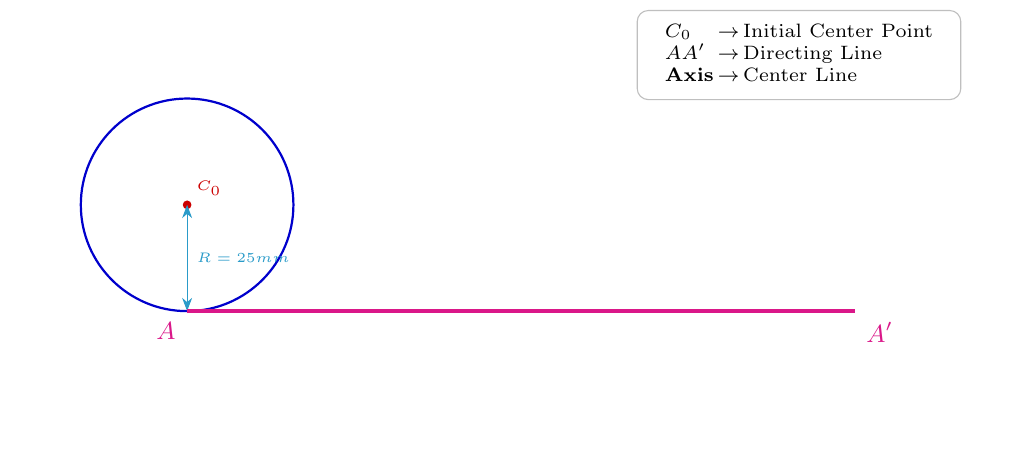
\begin{tikzpicture}[scale=0.45]
  \useasboundingbox (-4.5,-3.5) rectangle (22.5,8.0);
  \drawLegendCard{ \textbf{$C_0$} & Initial Center Point \\ \textbf{$AA'$} & Directing Line \\ \textbf{Axis} & Center Line }
  \coordinate (C0) at (0,3.0);
  \fill[red!80!black] (C0) circle (3.5pt) node[above right, font=\tiny] {$C_0$};
  \draw[thick, blue!80!black] (C0) circle (3.0);
  \draw[<->, thin, cyan!80!black] (0,3.0) -- (0,0) node[midway, right] {\tiny $R=25\text{ mm}$};
  \draw[directrix line] (0,0) node[below left] {\small $A$} -- (18.85,0) node[below right] {\small $A'$};
\end{tikzpicture}
\end{frame}

\begin{frame}{Step 1: Draw Generating Circle \& Directing Line}
\centering
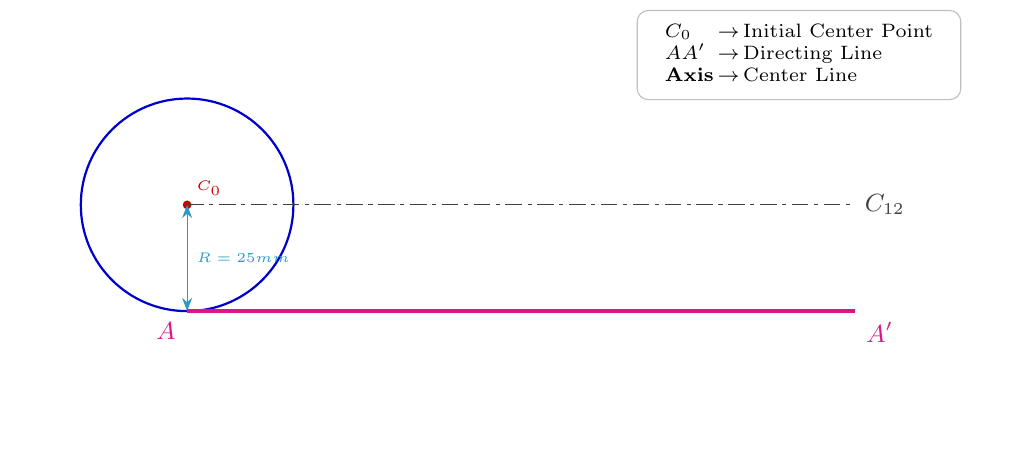
\begin{tikzpicture}[scale=0.45]
  \useasboundingbox (-4.5,-3.5) rectangle (22.5,8.0);
  \drawLegendCard{ \textbf{$C_0$} & Initial Center Point \\ \textbf{$AA'$} & Directing Line \\ \textbf{Axis} & Center Line }
  \coordinate (C0) at (0,3.0);
  \fill[red!80!black] (C0) circle (3.5pt) node[above right, font=\tiny] {$C_0$};
  \draw[thick, blue!80!black] (C0) circle (3.0);
  \draw[<->, thin, cyan!80!black] (0,3.0) -- (0,0) node[midway, right] {\tiny $R=25\text{ mm}$};
  \draw[directrix line] (0,0) node[below left] {\small $A$} -- (18.85,0) node[below right] {\small $A'$};
  \draw[axis line] (0,3.0) -- (18.85,3.0) node[right] {\small $C_{12}$};
\end{tikzpicture}
\end{frame}

\begin{frame}{Step 1: Draw Generating Circle \& Directing Line}
\centering
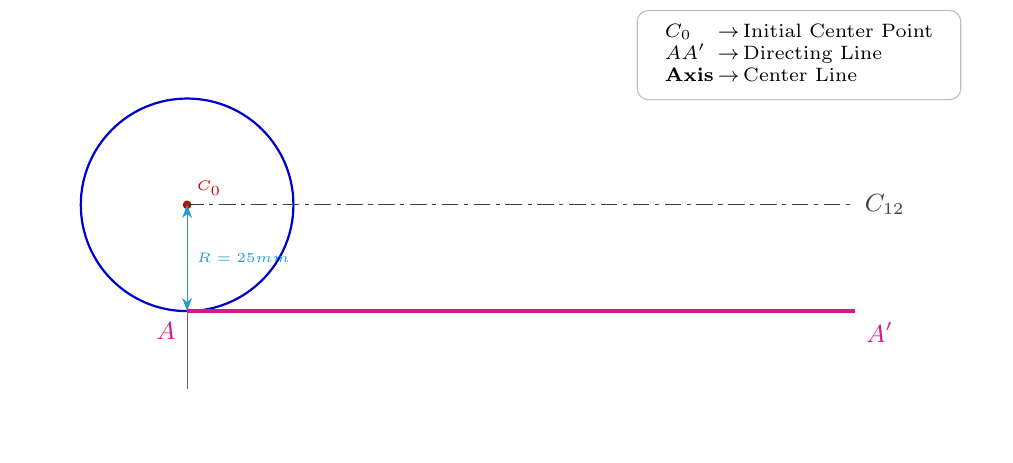
\begin{tikzpicture}[scale=0.45]
  \useasboundingbox (-4.5,-3.5) rectangle (22.5,8.0);
  \drawLegendCard{ \textbf{$C_0$} & Initial Center Point \\ \textbf{$AA'$} & Directing Line \\ \textbf{Axis} & Center Line }
  \coordinate (C0) at (0,3.0);
  \fill[red!80!black] (C0) circle (3.5pt) node[above right, font=\tiny] {$C_0$};
  \draw[thick, blue!80!black] (C0) circle (3.0);
  \draw[<->, thin, cyan!80!black] (0,3.0) -- (0,0) node[midway, right] {\tiny $R=25\text{ mm}$};
  \draw[directrix line] (0,0) node[below left] {\small $A$} -- (18.85,0) node[below right] {\small $A'$};
  \draw[axis line] (0,3.0) -- (18.85,3.0) node[right] {\small $C_{12}$};
  \draw[dimension extension] (0,0) -- (0,-2.2);
\end{tikzpicture}
\end{frame}

\begin{frame}{Step 1: Draw Generating Circle \& Directing Line}
\centering
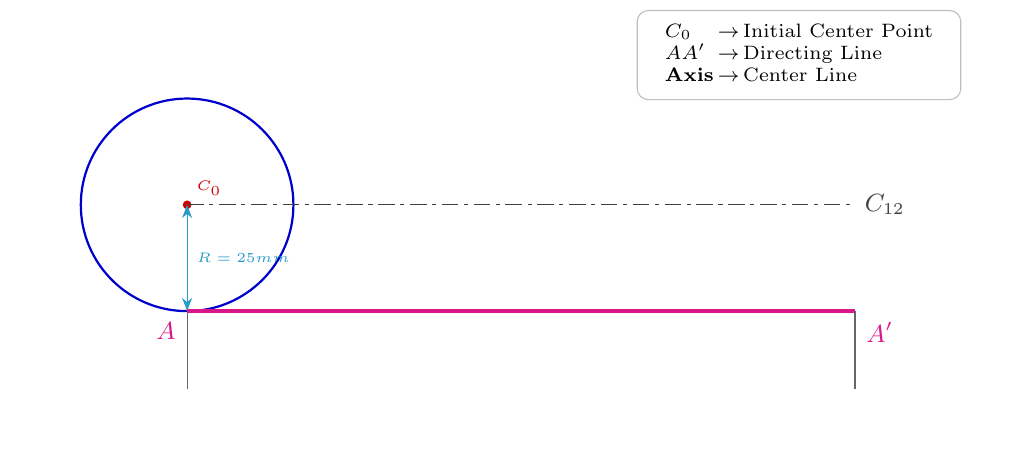
\begin{tikzpicture}[scale=0.45]
  \useasboundingbox (-4.5,-3.5) rectangle (22.5,8.0);
  \drawLegendCard{ \textbf{$C_0$} & Initial Center Point \\ \textbf{$AA'$} & Directing Line \\ \textbf{Axis} & Center Line }
  \coordinate (C0) at (0,3.0);
  \fill[red!80!black] (C0) circle (3.5pt) node[above right, font=\tiny] {$C_0$};
  \draw[thick, blue!80!black] (C0) circle (3.0);
  \draw[<->, thin, cyan!80!black] (0,3.0) -- (0,0) node[midway, right] {\tiny $R=25\text{ mm}$};
  \draw[directrix line] (0,0) node[below left] {\small $A$} -- (18.85,0) node[below right] {\small $A'$};
  \draw[axis line] (0,3.0) -- (18.85,3.0) node[right] {\small $C_{12}$};
  \draw[dimension extension] (0,0) -- (0,-2.2);
  \draw[dimension extension] (18.85,0) -- (18.85,-2.2);
\end{tikzpicture}
\end{frame}

\begin{frame}{Step 1: Draw Generating Circle \& Directing Line}
\centering
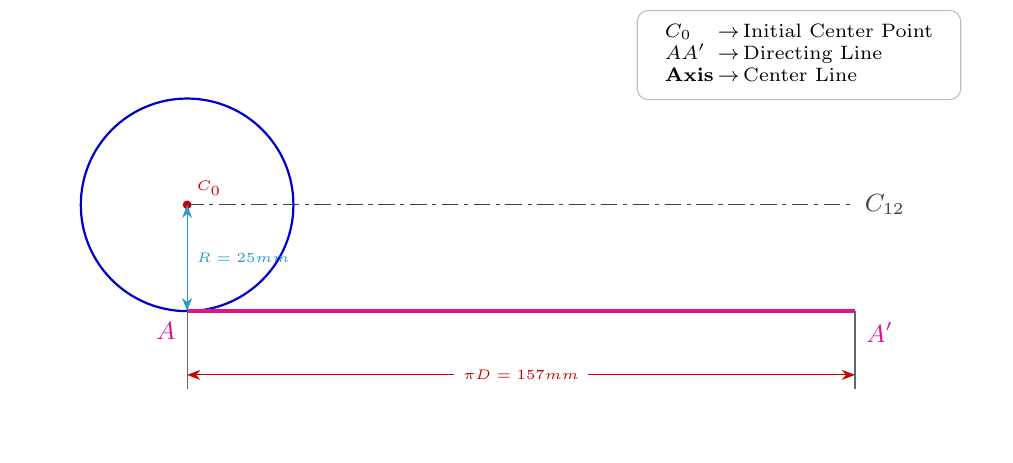
\begin{tikzpicture}[scale=0.45]
  \useasboundingbox (-4.5,-3.5) rectangle (22.5,8.0);
  \drawLegendCard{ \textbf{$C_0$} & Initial Center Point \\ \textbf{$AA'$} & Directing Line \\ \textbf{Axis} & Center Line }
  \coordinate (C0) at (0,3.0);
  \fill[red!80!black] (C0) circle (3.5pt) node[above right, font=\tiny] {$C_0$};
  \draw[thick, blue!80!black] (C0) circle (3.0);
  \draw[<->, thin, cyan!80!black] (0,3.0) -- (0,0) node[midway, right] {\tiny $R=25\text{ mm}$};
  \draw[directrix line] (0,0) node[below left] {\small $A$} -- (18.85,0) node[below right] {\small $A'$};
  \draw[axis line] (0,3.0) -- (18.85,3.0) node[right] {\small $C_{12}$};
  \draw[dimension extension] (0,0) -- (0,-2.2);
  \draw[dimension extension] (18.85,0) -- (18.85,-2.2);
  \draw[<->, red!80!black, thin] (0,-1.8) -- (18.85,-1.8) node[midway, fill=white] {\tiny $\pi D = 157\text{ mm}$};
\end{tikzpicture}
\end{frame}

\begin{frame}{Step 1: Draw Generating Circle \& Directing Line}
\centering
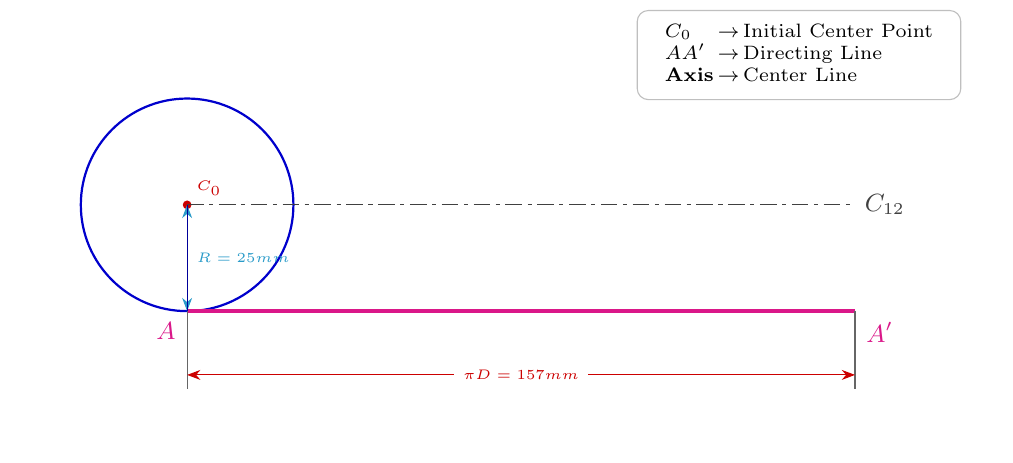
\begin{tikzpicture}[scale=0.45]
  \useasboundingbox (-4.5,-3.5) rectangle (22.5,8.0);
  \drawLegendCard{ \textbf{$C_0$} & Initial Center Point \\ \textbf{$AA'$} & Directing Line \\ \textbf{Axis} & Center Line }
  \coordinate (C0) at (0,3.0);
  \fill[red!80!black] (C0) circle (3.5pt) node[above right, font=\tiny] {$C_0$};
  \draw[thick, blue!80!black] (C0) circle (3.0);
  \draw[<->, thin, cyan!80!black] (0,3.0) -- (0,0) node[midway, right] {\tiny $R=25\text{ mm}$};
  \draw[directrix line] (0,0) node[below left] {\small $A$} -- (18.85,0) node[below right] {\small $A'$};
  \draw[axis line] (0,3.0) -- (18.85,3.0) node[right] {\small $C_{12}$};
  \draw[dimension extension] (0,0) -- (0,-2.2);
  \draw[dimension extension] (18.85,0) -- (18.85,-2.2);
  \draw[<->, red!80!black, thin] (0,-1.8) -- (18.85,-1.8) node[midway, fill=white] {\tiny $\pi D = 157\text{ mm}$};
  \draw[thin, construction line] (0,0) -- (C0);
\end{tikzpicture}
\end{frame}

% ============================================================
% STEP 2
% ============================================================
\renewcommand{\stepnum}{2}

\begin{frame}{Step 2: Divide Generating Circle into 12 Equal Parts}
\centering
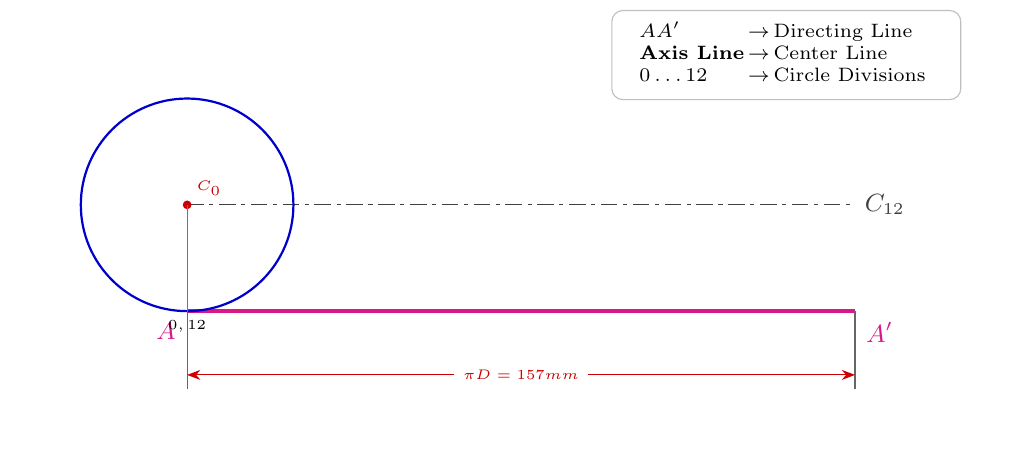
\begin{tikzpicture}[scale=0.45]
  \useasboundingbox (-4.5,-3.5) rectangle (22.5,8.0);
  \drawLegendCard{ \textbf{$AA'$} & Directing Line \\ \textbf{Axis Line} & Center Line \\ \textbf{$0\dots12$} & Circle Divisions }
  \draw[directrix line] (0,0) node[below left] {\small $A$} -- (18.85,0) node[below right] {\small $A'$};
  \draw[axis line] (0,3.0) -- (18.85,3.0) node[right] {\small $C_{12}$};
  \coordinate (C0) at (0,3.0);
  \fill[red!80!black] (C0) circle (3.5pt) node[above right, font=\tiny] {$C_0$};
  \draw[thick, blue!80!black] (C0) circle (3.0);
  \draw[thin, construction line] (0,0) -- (C0);
  \draw[dimension extension] (0,0) -- (0,-2.2);
  \draw[dimension extension] (18.85,0) -- (18.85,-2.2);
  \draw[<->, red!80!black, thin] (0,-1.8) -- (18.85,-1.8) node[midway, fill=white] {\tiny $\pi D = 157\text{ mm}$};
  \draw[thin, cyan!60!black, solid] (C0) -- (0,0); \node[below, font=\tiny] at (0,0) {$0, 12$};
\end{tikzpicture}
\end{frame}

\begin{frame}{Step 2: Divide Generating Circle into 12 Equal Parts}
\centering
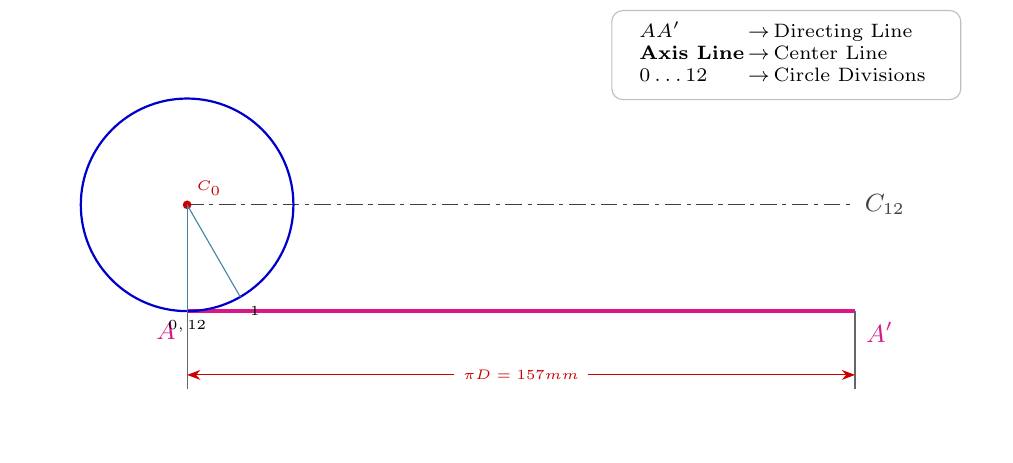
\begin{tikzpicture}[scale=0.45]
  \useasboundingbox (-4.5,-3.5) rectangle (22.5,8.0);
  \drawLegendCard{ \textbf{$AA'$} & Directing Line \\ \textbf{Axis Line} & Center Line \\ \textbf{$0\dots12$} & Circle Divisions }
  \draw[directrix line] (0,0) node[below left] {\small $A$} -- (18.85,0) node[below right] {\small $A'$};
  \draw[axis line] (0,3.0) -- (18.85,3.0) node[right] {\small $C_{12}$};
  \coordinate (C0) at (0,3.0);
  \fill[red!80!black] (C0) circle (3.5pt) node[above right, font=\tiny] {$C_0$};
  \draw[thick, blue!80!black] (C0) circle (3.0);
  \draw[thin, construction line] (0,0) -- (C0);
  \draw[dimension extension] (0,0) -- (0,-2.2);
  \draw[dimension extension] (18.85,0) -- (18.85,-2.2);
  \draw[<->, red!80!black, thin] (0,-1.8) -- (18.85,-1.8) node[midway, fill=white] {\tiny $\pi D = 157\text{ mm}$};
  \draw[thin, cyan!60!black, solid] (C0) -- (0,0); \node[below, font=\tiny] at (0,0) {$0, 12$};
  \draw[thin, cyan!60!black, solid] (C0) -- ++(300:3.0); \node[below right, font=\tiny] at (1.5,0.40) {1};
\end{tikzpicture}
\end{frame}

\begin{frame}{Step 2: Divide Generating Circle into 12 Equal Parts}
\centering
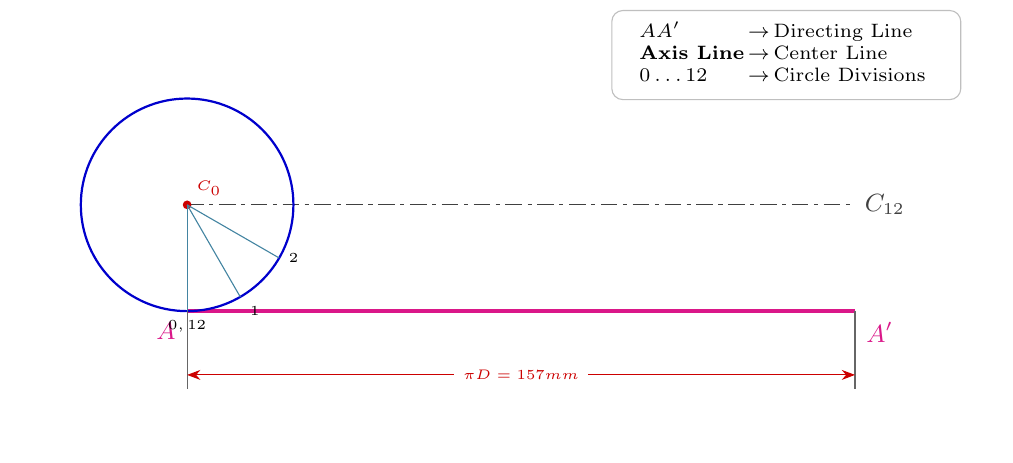
\begin{tikzpicture}[scale=0.45]
  \useasboundingbox (-4.5,-3.5) rectangle (22.5,8.0);
  \drawLegendCard{ \textbf{$AA'$} & Directing Line \\ \textbf{Axis Line} & Center Line \\ \textbf{$0\dots12$} & Circle Divisions }
  \draw[directrix line] (0,0) node[below left] {\small $A$} -- (18.85,0) node[below right] {\small $A'$};
  \draw[axis line] (0,3.0) -- (18.85,3.0) node[right] {\small $C_{12}$};
  \coordinate (C0) at (0,3.0);
  \fill[red!80!black] (C0) circle (3.5pt) node[above right, font=\tiny] {$C_0$};
  \draw[thick, blue!80!black] (C0) circle (3.0);
  \draw[thin, construction line] (0,0) -- (C0);
  \draw[dimension extension] (0,0) -- (0,-2.2);
  \draw[dimension extension] (18.85,0) -- (18.85,-2.2);
  \draw[<->, red!80!black, thin] (0,-1.8) -- (18.85,-1.8) node[midway, fill=white] {\tiny $\pi D = 157\text{ mm}$};
  \draw[thin, cyan!60!black, solid] (C0) -- (0,0); \node[below, font=\tiny] at (0,0) {$0, 12$};
  \draw[thin, cyan!60!black, solid] (C0) -- ++(300:3.0); \node[below right, font=\tiny] at (1.5,0.40) {1};
  \draw[thin, cyan!60!black, solid] (C0) -- ++(330:3.0); \node[right, font=\tiny] at (2.598,1.5) {2};
\end{tikzpicture}
\end{frame}

\begin{frame}{Step 2: Divide Generating Circle into 12 Equal Parts}
\centering
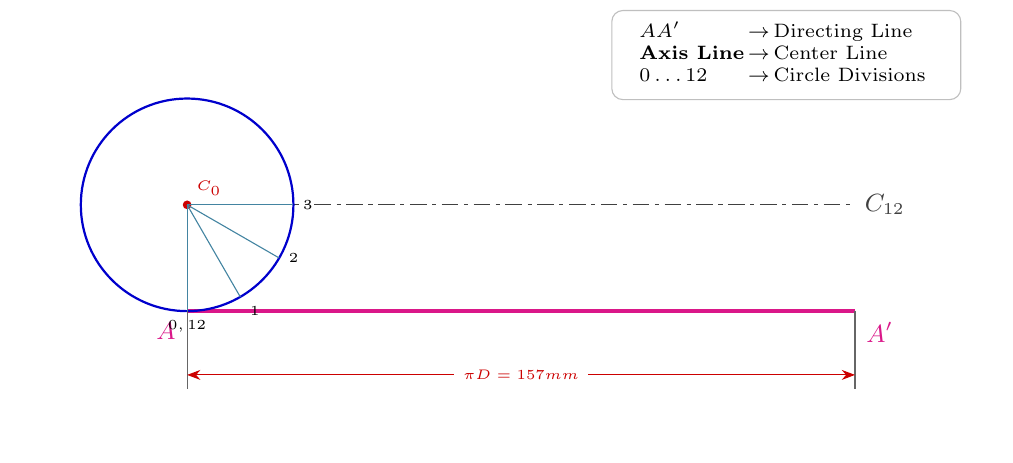
\begin{tikzpicture}[scale=0.45]
  \useasboundingbox (-4.5,-3.5) rectangle (22.5,8.0);
  \drawLegendCard{ \textbf{$AA'$} & Directing Line \\ \textbf{Axis Line} & Center Line \\ \textbf{$0\dots12$} & Circle Divisions }
  \draw[directrix line] (0,0) node[below left] {\small $A$} -- (18.85,0) node[below right] {\small $A'$};
  \draw[axis line] (0,3.0) -- (18.85,3.0) node[right] {\small $C_{12}$};
  \coordinate (C0) at (0,3.0);
  \fill[red!80!black] (C0) circle (3.5pt) node[above right, font=\tiny] {$C_0$};
  \draw[thick, blue!80!black] (C0) circle (3.0);
  \draw[thin, construction line] (0,0) -- (C0);
  \draw[dimension extension] (0,0) -- (0,-2.2);
  \draw[dimension extension] (18.85,0) -- (18.85,-2.2);
  \draw[<->, red!80!black, thin] (0,-1.8) -- (18.85,-1.8) node[midway, fill=white] {\tiny $\pi D = 157\text{ mm}$};
  \draw[thin, cyan!60!black, solid] (C0) -- (0,0); \node[below, font=\tiny] at (0,0) {$0, 12$};
  \draw[thin, cyan!60!black, solid] (C0) -- ++(300:3.0); \node[below right, font=\tiny] at (1.5,0.40) {1};
  \draw[thin, cyan!60!black, solid] (C0) -- ++(330:3.0); \node[right, font=\tiny] at (2.598,1.5) {2};
  \draw[thin, cyan!60!black, solid] (C0) -- ++(0:3.0); \node[right, font=\tiny] at (3.0,3.0) {3};
\end{tikzpicture}
\end{frame}

\begin{frame}{Step 2: Divide Generating Circle into 12 Equal Parts}
\centering
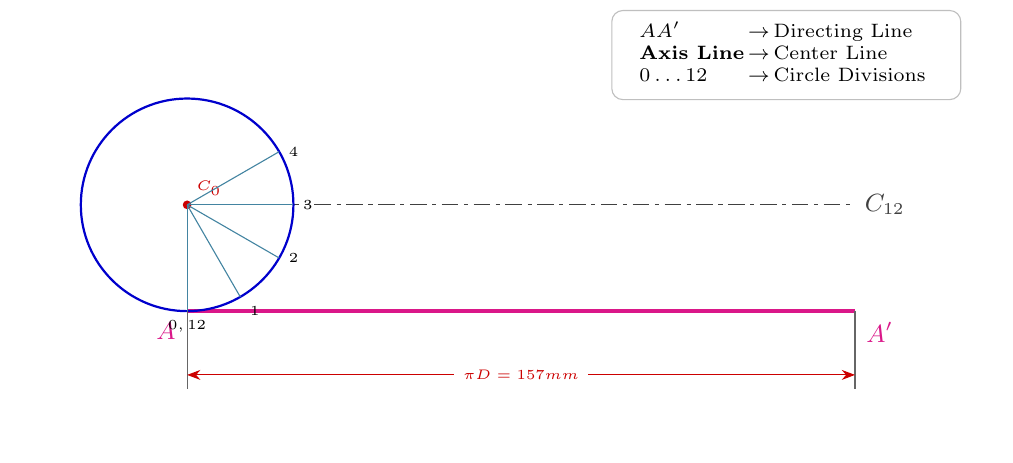
\begin{tikzpicture}[scale=0.45]
  \useasboundingbox (-4.5,-3.5) rectangle (22.5,8.0);
  \drawLegendCard{ \textbf{$AA'$} & Directing Line \\ \textbf{Axis Line} & Center Line \\ \textbf{$0\dots12$} & Circle Divisions }
  \draw[directrix line] (0,0) node[below left] {\small $A$} -- (18.85,0) node[below right] {\small $A'$};
  \draw[axis line] (0,3.0) -- (18.85,3.0) node[right] {\small $C_{12}$};
  \coordinate (C0) at (0,3.0);
  \fill[red!80!black] (C0) circle (3.5pt) node[above right, font=\tiny] {$C_0$};
  \draw[thick, blue!80!black] (C0) circle (3.0);
  \draw[thin, construction line] (0,0) -- (C0);
  \draw[dimension extension] (0,0) -- (0,-2.2);
  \draw[dimension extension] (18.85,0) -- (18.85,-2.2);
  \draw[<->, red!80!black, thin] (0,-1.8) -- (18.85,-1.8) node[midway, fill=white] {\tiny $\pi D = 157\text{ mm}$};
  \draw[thin, cyan!60!black, solid] (C0) -- (0,0); \node[below, font=\tiny] at (0,0) {$0, 12$};
  \draw[thin, cyan!60!black, solid] (C0) -- ++(300:3.0); \node[below right, font=\tiny] at (1.5,0.40) {1};
  \draw[thin, cyan!60!black, solid] (C0) -- ++(330:3.0); \node[right, font=\tiny] at (2.598,1.5) {2};
  \draw[thin, cyan!60!black, solid] (C0) -- ++(0:3.0); \node[right, font=\tiny] at (3.0,3.0) {3};
  \draw[thin, cyan!60!black, solid] (C0) -- ++(30:3.0); \node[right, font=\tiny] at (2.598,4.5) {4};
\end{tikzpicture}
\end{frame}

\begin{frame}{Step 2: Divide Generating Circle into 12 Equal Parts}
\centering
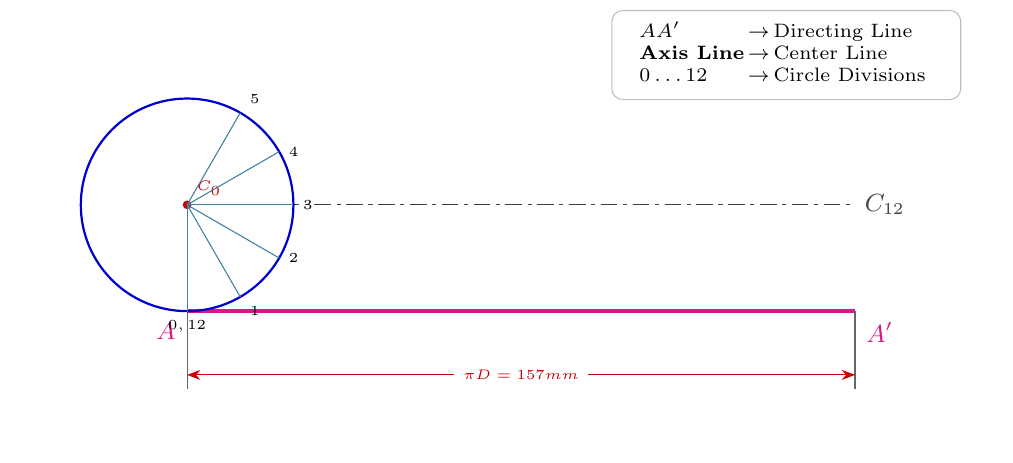
\begin{tikzpicture}[scale=0.45]
  \useasboundingbox (-4.5,-3.5) rectangle (22.5,8.0);
  \drawLegendCard{ \textbf{$AA'$} & Directing Line \\ \textbf{Axis Line} & Center Line \\ \textbf{$0\dots12$} & Circle Divisions }
  \draw[directrix line] (0,0) node[below left] {\small $A$} -- (18.85,0) node[below right] {\small $A'$};
  \draw[axis line] (0,3.0) -- (18.85,3.0) node[right] {\small $C_{12}$};
  \coordinate (C0) at (0,3.0);
  \fill[red!80!black] (C0) circle (3.5pt) node[above right, font=\tiny] {$C_0$};
  \draw[thick, blue!80!black] (C0) circle (3.0);
  \draw[thin, construction line] (0,0) -- (C0);
  \draw[dimension extension] (0,0) -- (0,-2.2);
  \draw[dimension extension] (18.85,0) -- (18.85,-2.2);
  \draw[<->, red!80!black, thin] (0,-1.8) -- (18.85,-1.8) node[midway, fill=white] {\tiny $\pi D = 157\text{ mm}$};
  \draw[thin, cyan!60!black, solid] (C0) -- (0,0); \node[below, font=\tiny] at (0,0) {$0, 12$};
  \draw[thin, cyan!60!black, solid] (C0) -- ++(300:3.0); \node[below right, font=\tiny] at (1.5,0.40) {1};
  \draw[thin, cyan!60!black, solid] (C0) -- ++(330:3.0); \node[right, font=\tiny] at (2.598,1.5) {2};
  \draw[thin, cyan!60!black, solid] (C0) -- ++(0:3.0); \node[right, font=\tiny] at (3.0,3.0) {3};
  \draw[thin, cyan!60!black, solid] (C0) -- ++(30:3.0); \node[right, font=\tiny] at (2.598,4.5) {4};
  \draw[thin, cyan!60!black, solid] (C0) -- ++(60:3.0); \node[above right, font=\tiny] at (1.5,5.598) {5};
\end{tikzpicture}
\end{frame}

\begin{frame}{Step 2: Divide Generating Circle into 12 Equal Parts}
\centering
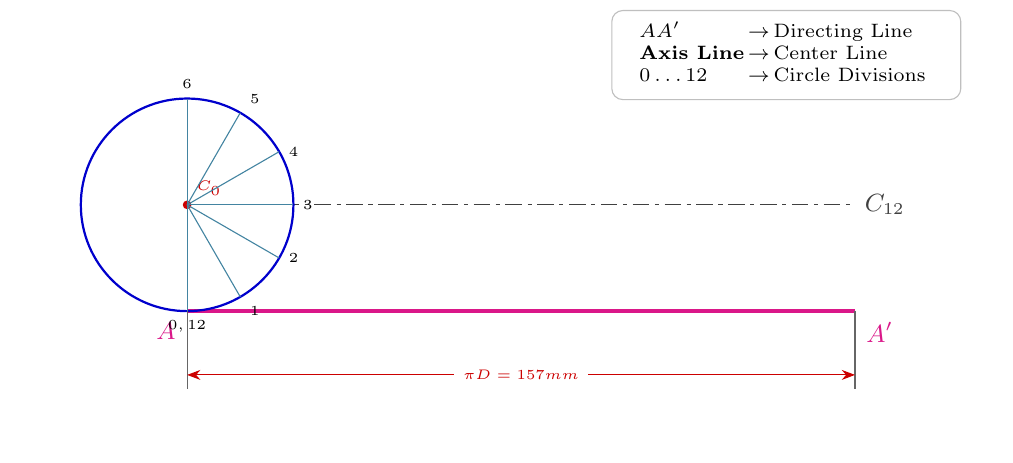
\begin{tikzpicture}[scale=0.45]
  \useasboundingbox (-4.5,-3.5) rectangle (22.5,8.0);
  \drawLegendCard{ \textbf{$AA'$} & Directing Line \\ \textbf{Axis Line} & Center Line \\ \textbf{$0\dots12$} & Circle Divisions }
  \draw[directrix line] (0,0) node[below left] {\small $A$} -- (18.85,0) node[below right] {\small $A'$};
  \draw[axis line] (0,3.0) -- (18.85,3.0) node[right] {\small $C_{12}$};
  \coordinate (C0) at (0,3.0);
  \fill[red!80!black] (C0) circle (3.5pt) node[above right, font=\tiny] {$C_0$};
  \draw[thick, blue!80!black] (C0) circle (3.0);
  \draw[thin, construction line] (0,0) -- (C0);
  \draw[dimension extension] (0,0) -- (0,-2.2);
  \draw[dimension extension] (18.85,0) -- (18.85,-2.2);
  \draw[<->, red!80!black, thin] (0,-1.8) -- (18.85,-1.8) node[midway, fill=white] {\tiny $\pi D = 157\text{ mm}$};
  \draw[thin, cyan!60!black, solid] (C0) -- (0,0); \node[below, font=\tiny] at (0,0) {$0, 12$};
  \draw[thin, cyan!60!black, solid] (C0) -- ++(300:3.0); \node[below right, font=\tiny] at (1.5,0.40) {1};
  \draw[thin, cyan!60!black, solid] (C0) -- ++(330:3.0); \node[right, font=\tiny] at (2.598,1.5) {2};
  \draw[thin, cyan!60!black, solid] (C0) -- ++(0:3.0); \node[right, font=\tiny] at (3.0,3.0) {3};
  \draw[thin, cyan!60!black, solid] (C0) -- ++(30:3.0); \node[right, font=\tiny] at (2.598,4.5) {4};
  \draw[thin, cyan!60!black, solid] (C0) -- ++(60:3.0); \node[above right, font=\tiny] at (1.5,5.598) {5};
  \draw[thin, cyan!60!black, solid] (C0) -- ++(90:3.0); \node[above, font=\tiny] at (0,6.0) {6};
\end{tikzpicture}
\end{frame}

\begin{frame}{Step 2: Divide Generating Circle into 12 Equal Parts}
\centering
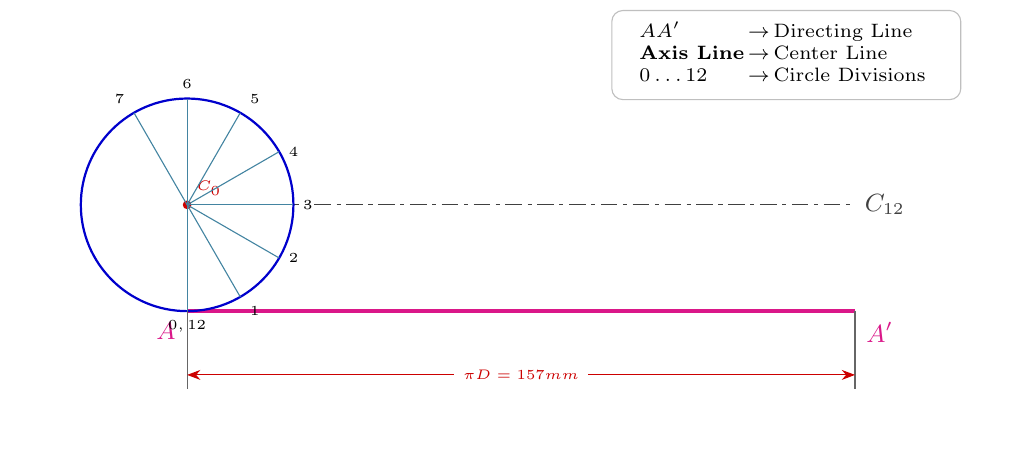
\begin{tikzpicture}[scale=0.45]
  \useasboundingbox (-4.5,-3.5) rectangle (22.5,8.0);
  \drawLegendCard{ \textbf{$AA'$} & Directing Line \\ \textbf{Axis Line} & Center Line \\ \textbf{$0\dots12$} & Circle Divisions }
  \draw[directrix line] (0,0) node[below left] {\small $A$} -- (18.85,0) node[below right] {\small $A'$};
  \draw[axis line] (0,3.0) -- (18.85,3.0) node[right] {\small $C_{12}$};
  \coordinate (C0) at (0,3.0);
  \fill[red!80!black] (C0) circle (3.5pt) node[above right, font=\tiny] {$C_0$};
  \draw[thick, blue!80!black] (C0) circle (3.0);
  \draw[thin, construction line] (0,0) -- (C0);
  \draw[dimension extension] (0,0) -- (0,-2.2);
  \draw[dimension extension] (18.85,0) -- (18.85,-2.2);
  \draw[<->, red!80!black, thin] (0,-1.8) -- (18.85,-1.8) node[midway, fill=white] {\tiny $\pi D = 157\text{ mm}$};
  \draw[thin, cyan!60!black, solid] (C0) -- (0,0); \node[below, font=\tiny] at (0,0) {$0, 12$};
  \draw[thin, cyan!60!black, solid] (C0) -- ++(300:3.0); \node[below right, font=\tiny] at (1.5,0.40) {1};
  \draw[thin, cyan!60!black, solid] (C0) -- ++(330:3.0); \node[right, font=\tiny] at (2.598,1.5) {2};
  \draw[thin, cyan!60!black, solid] (C0) -- ++(0:3.0); \node[right, font=\tiny] at (3.0,3.0) {3};
  \draw[thin, cyan!60!black, solid] (C0) -- ++(30:3.0); \node[right, font=\tiny] at (2.598,4.5) {4};
  \draw[thin, cyan!60!black, solid] (C0) -- ++(60:3.0); \node[above right, font=\tiny] at (1.5,5.598) {5};
  \draw[thin, cyan!60!black, solid] (C0) -- ++(90:3.0); \node[above, font=\tiny] at (0,6.0) {6};
  \draw[thin, cyan!60!black, solid] (C0) -- ++(120:3.0); \node[above left, font=\tiny] at (-1.5,5.598) {7};
\end{tikzpicture}
\end{frame}

\begin{frame}{Step 2: Divide Generating Circle into 12 Equal Parts}
\centering
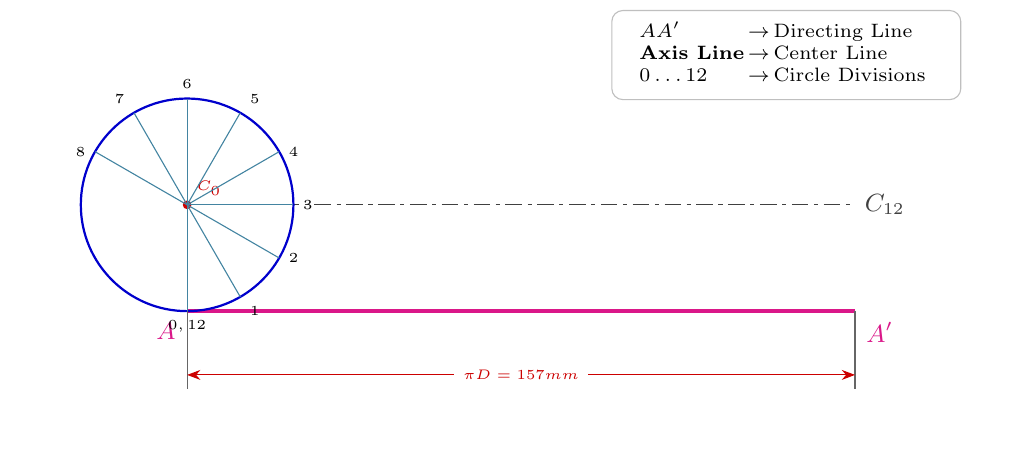
\begin{tikzpicture}[scale=0.45]
  \useasboundingbox (-4.5,-3.5) rectangle (22.5,8.0);
  \drawLegendCard{ \textbf{$AA'$} & Directing Line \\ \textbf{Axis Line} & Center Line \\ \textbf{$0\dots12$} & Circle Divisions }
  \draw[directrix line] (0,0) node[below left] {\small $A$} -- (18.85,0) node[below right] {\small $A'$};
  \draw[axis line] (0,3.0) -- (18.85,3.0) node[right] {\small $C_{12}$};
  \coordinate (C0) at (0,3.0);
  \fill[red!80!black] (C0) circle (3.5pt) node[above right, font=\tiny] {$C_0$};
  \draw[thick, blue!80!black] (C0) circle (3.0);
  \draw[thin, construction line] (0,0) -- (C0);
  \draw[dimension extension] (0,0) -- (0,-2.2);
  \draw[dimension extension] (18.85,0) -- (18.85,-2.2);
  \draw[<->, red!80!black, thin] (0,-1.8) -- (18.85,-1.8) node[midway, fill=white] {\tiny $\pi D = 157\text{ mm}$};
  \draw[thin, cyan!60!black, solid] (C0) -- (0,0); \node[below, font=\tiny] at (0,0) {$0, 12$};
  \draw[thin, cyan!60!black, solid] (C0) -- ++(300:3.0); \node[below right, font=\tiny] at (1.5,0.40) {1};
  \draw[thin, cyan!60!black, solid] (C0) -- ++(330:3.0); \node[right, font=\tiny] at (2.598,1.5) {2};
  \draw[thin, cyan!60!black, solid] (C0) -- ++(0:3.0); \node[right, font=\tiny] at (3.0,3.0) {3};
  \draw[thin, cyan!60!black, solid] (C0) -- ++(30:3.0); \node[right, font=\tiny] at (2.598,4.5) {4};
  \draw[thin, cyan!60!black, solid] (C0) -- ++(60:3.0); \node[above right, font=\tiny] at (1.5,5.598) {5};
  \draw[thin, cyan!60!black, solid] (C0) -- ++(90:3.0); \node[above, font=\tiny] at (0,6.0) {6};
  \draw[thin, cyan!60!black, solid] (C0) -- ++(120:3.0); \node[above left, font=\tiny] at (-1.5,5.598) {7};
  \draw[thin, cyan!60!black, solid] (C0) -- ++(150:3.0); \node[left, font=\tiny] at (-2.598,4.5) {8};
\end{tikzpicture}
\end{frame}

\begin{frame}{Step 2: Divide Generating Circle into 12 Equal Parts}
\centering
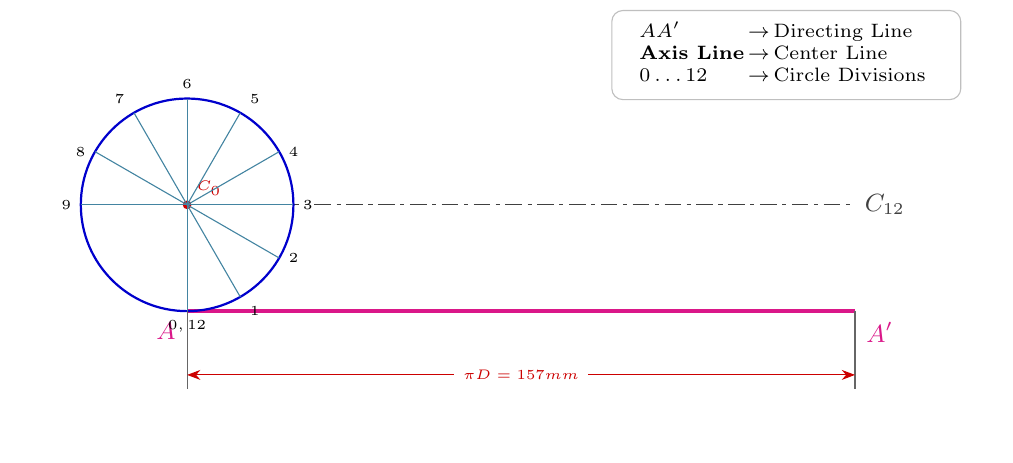
\begin{tikzpicture}[scale=0.45]
  \useasboundingbox (-4.5,-3.5) rectangle (22.5,8.0);
  \drawLegendCard{ \textbf{$AA'$} & Directing Line \\ \textbf{Axis Line} & Center Line \\ \textbf{$0\dots12$} & Circle Divisions }
  \draw[directrix line] (0,0) node[below left] {\small $A$} -- (18.85,0) node[below right] {\small $A'$};
  \draw[axis line] (0,3.0) -- (18.85,3.0) node[right] {\small $C_{12}$};
  \coordinate (C0) at (0,3.0);
  \fill[red!80!black] (C0) circle (3.5pt) node[above right, font=\tiny] {$C_0$};
  \draw[thick, blue!80!black] (C0) circle (3.0);
  \draw[thin, construction line] (0,0) -- (C0);
  \draw[dimension extension] (0,0) -- (0,-2.2);
  \draw[dimension extension] (18.85,0) -- (18.85,-2.2);
  \draw[<->, red!80!black, thin] (0,-1.8) -- (18.85,-1.8) node[midway, fill=white] {\tiny $\pi D = 157\text{ mm}$};
  \draw[thin, cyan!60!black, solid] (C0) -- (0,0); \node[below, font=\tiny] at (0,0) {$0, 12$};
  \draw[thin, cyan!60!black, solid] (C0) -- ++(300:3.0); \node[below right, font=\tiny] at (1.5,0.40) {1};
  \draw[thin, cyan!60!black, solid] (C0) -- ++(330:3.0); \node[right, font=\tiny] at (2.598,1.5) {2};
  \draw[thin, cyan!60!black, solid] (C0) -- ++(0:3.0); \node[right, font=\tiny] at (3.0,3.0) {3};
  \draw[thin, cyan!60!black, solid] (C0) -- ++(30:3.0); \node[right, font=\tiny] at (2.598,4.5) {4};
  \draw[thin, cyan!60!black, solid] (C0) -- ++(60:3.0); \node[above right, font=\tiny] at (1.5,5.598) {5};
  \draw[thin, cyan!60!black, solid] (C0) -- ++(90:3.0); \node[above, font=\tiny] at (0,6.0) {6};
  \draw[thin, cyan!60!black, solid] (C0) -- ++(120:3.0); \node[above left, font=\tiny] at (-1.5,5.598) {7};
  \draw[thin, cyan!60!black, solid] (C0) -- ++(150:3.0); \node[left, font=\tiny] at (-2.598,4.5) {8};
  \draw[thin, cyan!60!black, solid] (C0) -- ++(180:3.0); \node[left, font=\tiny] at (-3.0,3.0) {9};
\end{tikzpicture}
\end{frame}

\begin{frame}{Step 2: Divide Generating Circle into 12 Equal Parts}
\centering
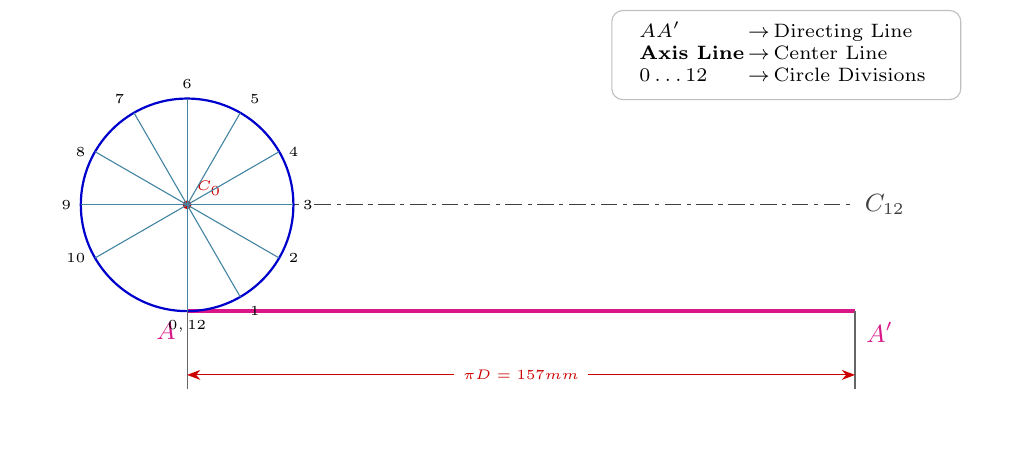
\begin{tikzpicture}[scale=0.45]
  \useasboundingbox (-4.5,-3.5) rectangle (22.5,8.0);
  \drawLegendCard{ \textbf{$AA'$} & Directing Line \\ \textbf{Axis Line} & Center Line \\ \textbf{$0\dots12$} & Circle Divisions }
  \draw[directrix line] (0,0) node[below left] {\small $A$} -- (18.85,0) node[below right] {\small $A'$};
  \draw[axis line] (0,3.0) -- (18.85,3.0) node[right] {\small $C_{12}$};
  \coordinate (C0) at (0,3.0);
  \fill[red!80!black] (C0) circle (3.5pt) node[above right, font=\tiny] {$C_0$};
  \draw[thick, blue!80!black] (C0) circle (3.0);
  \draw[thin, construction line] (0,0) -- (C0);
  \draw[dimension extension] (0,0) -- (0,-2.2);
  \draw[dimension extension] (18.85,0) -- (18.85,-2.2);
  \draw[<->, red!80!black, thin] (0,-1.8) -- (18.85,-1.8) node[midway, fill=white] {\tiny $\pi D = 157\text{ mm}$};
  \draw[thin, cyan!60!black, solid] (C0) -- (0,0); \node[below, font=\tiny] at (0,0) {$0, 12$};
  \draw[thin, cyan!60!black, solid] (C0) -- ++(300:3.0); \node[below right, font=\tiny] at (1.5,0.40) {1};
  \draw[thin, cyan!60!black, solid] (C0) -- ++(330:3.0); \node[right, font=\tiny] at (2.598,1.5) {2};
  \draw[thin, cyan!60!black, solid] (C0) -- ++(0:3.0); \node[right, font=\tiny] at (3.0,3.0) {3};
  \draw[thin, cyan!60!black, solid] (C0) -- ++(30:3.0); \node[right, font=\tiny] at (2.598,4.5) {4};
  \draw[thin, cyan!60!black, solid] (C0) -- ++(60:3.0); \node[above right, font=\tiny] at (1.5,5.598) {5};
  \draw[thin, cyan!60!black, solid] (C0) -- ++(90:3.0); \node[above, font=\tiny] at (0,6.0) {6};
  \draw[thin, cyan!60!black, solid] (C0) -- ++(120:3.0); \node[above left, font=\tiny] at (-1.5,5.598) {7};
  \draw[thin, cyan!60!black, solid] (C0) -- ++(150:3.0); \node[left, font=\tiny] at (-2.598,4.5) {8};
  \draw[thin, cyan!60!black, solid] (C0) -- ++(180:3.0); \node[left, font=\tiny] at (-3.0,3.0) {9};
  \draw[thin, cyan!60!black, solid] (C0) -- ++(210:3.0); \node[left, font=\tiny] at (-2.598,1.5) {10};
\end{tikzpicture}
\end{frame}

\begin{frame}{Step 2: Divide Generating Circle into 12 Equal Parts}
\centering
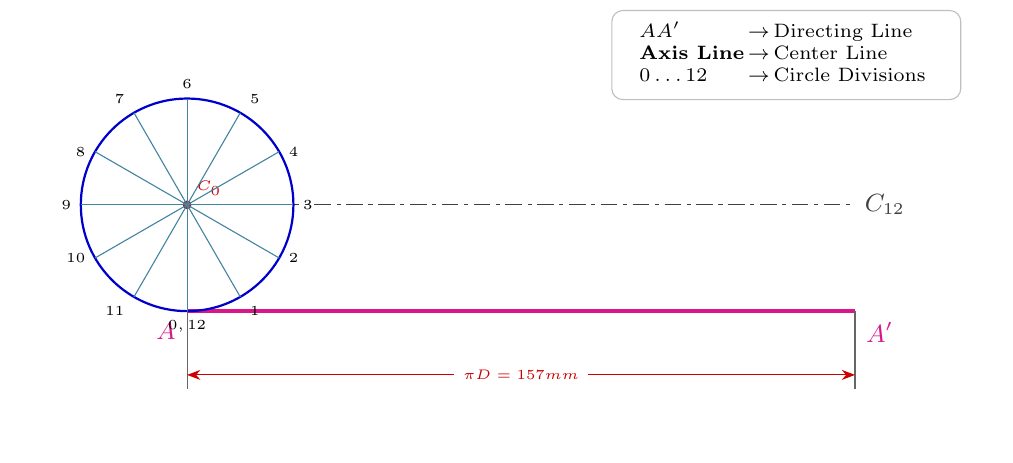
\begin{tikzpicture}[scale=0.45]
  \useasboundingbox (-4.5,-3.5) rectangle (22.5,8.0);
  \drawLegendCard{ \textbf{$AA'$} & Directing Line \\ \textbf{Axis Line} & Center Line \\ \textbf{$0\dots12$} & Circle Divisions }
  \draw[directrix line] (0,0) node[below left] {\small $A$} -- (18.85,0) node[below right] {\small $A'$};
  \draw[axis line] (0,3.0) -- (18.85,3.0) node[right] {\small $C_{12}$};
  \coordinate (C0) at (0,3.0);
  \fill[red!80!black] (C0) circle (3.5pt) node[above right, font=\tiny] {$C_0$};
  \draw[thick, blue!80!black] (C0) circle (3.0);
  \draw[thin, construction line] (0,0) -- (C0);
  \draw[dimension extension] (0,0) -- (0,-2.2);
  \draw[dimension extension] (18.85,0) -- (18.85,-2.2);
  \draw[<->, red!80!black, thin] (0,-1.8) -- (18.85,-1.8) node[midway, fill=white] {\tiny $\pi D = 157\text{ mm}$};
  \draw[thin, cyan!60!black, solid] (C0) -- (0,0); \node[below, font=\tiny] at (0,0) {$0, 12$};
  \draw[thin, cyan!60!black, solid] (C0) -- ++(300:3.0); \node[below right, font=\tiny] at (1.5,0.40) {1};
  \draw[thin, cyan!60!black, solid] (C0) -- ++(330:3.0); \node[right, font=\tiny] at (2.598,1.5) {2};
  \draw[thin, cyan!60!black, solid] (C0) -- ++(0:3.0); \node[right, font=\tiny] at (3.0,3.0) {3};
  \draw[thin, cyan!60!black, solid] (C0) -- ++(30:3.0); \node[right, font=\tiny] at (2.598,4.5) {4};
  \draw[thin, cyan!60!black, solid] (C0) -- ++(60:3.0); \node[above right, font=\tiny] at (1.5,5.598) {5};
  \draw[thin, cyan!60!black, solid] (C0) -- ++(90:3.0); \node[above, font=\tiny] at (0,6.0) {6};
  \draw[thin, cyan!60!black, solid] (C0) -- ++(120:3.0); \node[above left, font=\tiny] at (-1.5,5.598) {7};
  \draw[thin, cyan!60!black, solid] (C0) -- ++(150:3.0); \node[left, font=\tiny] at (-2.598,4.5) {8};
  \draw[thin, cyan!60!black, solid] (C0) -- ++(180:3.0); \node[left, font=\tiny] at (-3.0,3.0) {9};
  \draw[thin, cyan!60!black, solid] (C0) -- ++(210:3.0); \node[left, font=\tiny] at (-2.598,1.5) {10};
  \draw[thin, cyan!60!black, solid] (C0) -- ++(240:3.0); \node[below left, font=\tiny] at (-1.5,0.40) {11};
\end{tikzpicture}
\end{frame}

% ============================================================
% STEP 3: DIVIDE DIRECTING LINE (Sequential Transfer Animation Slides)
% ============================================================
\renewcommand{\stepnum}{3}

\begin{frame}{Step 3: Divide Directing Line - Setup Inclined Line $AX$}
\centering
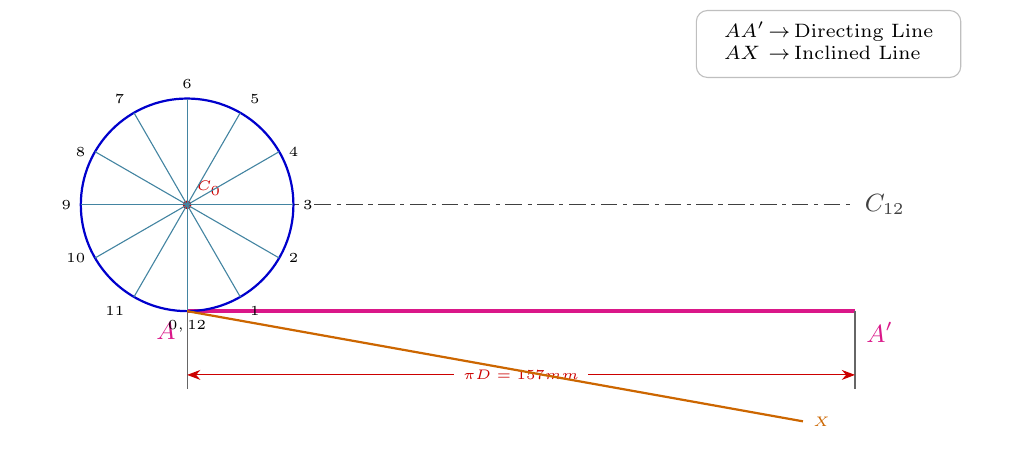
\begin{tikzpicture}[scale=0.45]
  \useasboundingbox (-4.5,-3.5) rectangle (22.5,8.0);
  \drawLegendCard{ \textbf{$AA'$} & Directing Line \\ \textbf{$A X$} & Inclined Line }
  \draw[directrix line] (0,0) node[below left] {\small $A$} -- (18.85,0) node[below right] {\small $A'$};
  \draw[axis line] (0,3.0) -- (18.85,3.0) node[right] {\small $C_{12}$};
  \coordinate (C0) at (0,3.0);
  \fill[red!80!black] (C0) circle (3.5pt) node[above right, font=\tiny] {$C_0$};
  \draw[thick, blue!80!black] (C0) circle (3.0);
  \draw[thin, construction line] (0,0) -- (C0);
  \draw[thin, cyan!60!black, solid] (C0) -- (0,0);
  \draw[thin, cyan!60!black, solid] (C0) -- ++(300:3.0);
  \draw[thin, cyan!60!black, solid] (C0) -- ++(330:3.0);
  \draw[thin, cyan!60!black, solid] (C0) -- ++(0:3.0);
  \draw[thin, cyan!60!black, solid] (C0) -- ++(30:3.0);
  \draw[thin, cyan!60!black, solid] (C0) -- ++(60:3.0);
  \draw[thin, cyan!60!black, solid] (C0) -- ++(90:3.0);
  \draw[thin, cyan!60!black, solid] (C0) -- ++(120:3.0);
  \draw[thin, cyan!60!black, solid] (C0) -- ++(150:3.0);
  \draw[thin, cyan!60!black, solid] (C0) -- ++(180:3.0);
  \draw[thin, cyan!60!black, solid] (C0) -- ++(210:3.0);
  \draw[thin, cyan!60!black, solid] (C0) -- ++(240:3.0);
  \node[below, font=\tiny] at (0,0) {$0, 12$};
  \node[below right, font=\tiny] at (1.5,0.40) {1};
  \node[right, font=\tiny] at (2.598,1.5) {2};
  \node[right, font=\tiny] at (3.0,3.0) {3};
  \node[right, font=\tiny] at (2.598,4.5) {4};
  \node[above right, font=\tiny] at (1.5,5.598) {5};
  \node[above, font=\tiny] at (0,6.0) {6};
  \node[above left, font=\tiny] at (-1.5,5.598) {7};
  \node[left, font=\tiny] at (-2.598,4.5) {8};
  \node[left, font=\tiny] at (-3.0,3.0) {9};
  \node[left, font=\tiny] at (-2.598,1.5) {10};
  \node[below left, font=\tiny] at (-1.5,0.40) {11};
  \draw[dimension extension] (0,0) -- (0,-2.2);
  \draw[dimension extension] (18.85,0) -- (18.85,-2.2);
  \draw[<->, red!80!black, thin] (0,-1.8) -- (18.85,-1.8) node[midway, fill=white] {\tiny $\pi D = 157\text{ mm}$};
  \draw[thick, orange!80!black] (0,0) -- (17.38,-3.11) node[right, font=\tiny] {$X$};
\end{tikzpicture}
\end{frame}

\begin{frame}{Step 3: Divide Directing Line - Add Numbers on Line $AX$}
\centering
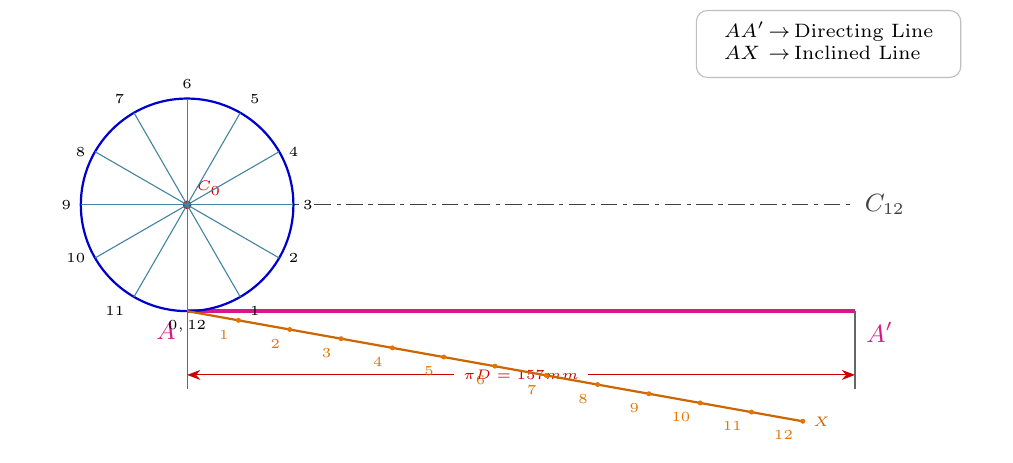
\begin{tikzpicture}[scale=0.45]
  \useasboundingbox (-4.5,-3.5) rectangle (22.5,8.0);
  \drawLegendCard{ \textbf{$AA'$} & Directing Line \\ \textbf{$A X$} & Inclined Line }
  \draw[directrix line] (0,0) node[below left] {\small $A$} -- (18.85,0) node[below right] {\small $A'$};
  \draw[axis line] (0,3.0) -- (18.85,3.0) node[right] {\small $C_{12}$};
  \coordinate (C0) at (0,3.0);
  \fill[red!80!black] (C0) circle (3.5pt) node[above right, font=\tiny] {$C_0$};
  \draw[thick, blue!80!black] (C0) circle (3.0);
  \draw[thin, construction line] (0,0) -- (C0);
  \draw[thin, cyan!60!black, solid] (C0) -- (0,0);
  \draw[thin, cyan!60!black, solid] (C0) -- ++(300:3.0);
  \draw[thin, cyan!60!black, solid] (C0) -- ++(330:3.0);
  \draw[thin, cyan!60!black, solid] (C0) -- ++(0:3.0);
  \draw[thin, cyan!60!black, solid] (C0) -- ++(30:3.0);
  \draw[thin, cyan!60!black, solid] (C0) -- ++(60:3.0);
  \draw[thin, cyan!60!black, solid] (C0) -- ++(90:3.0);
  \draw[thin, cyan!60!black, solid] (C0) -- ++(120:3.0);
  \draw[thin, cyan!60!black, solid] (C0) -- ++(150:3.0);
  \draw[thin, cyan!60!black, solid] (C0) -- ++(180:3.0);
  \draw[thin, cyan!60!black, solid] (C0) -- ++(210:3.0);
  \draw[thin, cyan!60!black, solid] (C0) -- ++(240:3.0);
  \node[below, font=\tiny] at (0,0) {$0, 12$};
  \node[below right, font=\tiny] at (1.5,0.40) {1};
  \node[right, font=\tiny] at (2.598,1.5) {2};
  \node[right, font=\tiny] at (3.0,3.0) {3};
  \node[right, font=\tiny] at (2.598,4.5) {4};
  \node[above right, font=\tiny] at (1.5,5.598) {5};
  \node[above, font=\tiny] at (0,6.0) {6};
  \node[above left, font=\tiny] at (-1.5,5.598) {7};
  \node[left, font=\tiny] at (-2.598,4.5) {8};
  \node[left, font=\tiny] at (-3.0,3.0) {9};
  \node[left, font=\tiny] at (-2.598,1.5) {10};
  \node[below left, font=\tiny] at (-1.5,0.40) {11};
  \draw[dimension extension] (0,0) -- (0,-2.2);
  \draw[dimension extension] (18.85,0) -- (18.85,-2.2);
  \draw[<->, red!80!black, thin] (0,-1.8) -- (18.85,-1.8) node[midway, fill=white] {\tiny $\pi D = 157\text{ mm}$};
  \draw[thick, orange!80!black] (0,0) -- (17.38,-3.11) node[right, font=\tiny] {$X$};
  \foreach \i in {1,2,...,12} {
    \coordinate (a\i) at ({\i*1.448}, {-\i*0.259});
    \fill[orange!90!black] (a\i) circle (2.0pt);
    \node[below left, font=\tiny, orange!90!black] at (a\i) {\i};
  }
\end{tikzpicture}
\end{frame}

\begin{frame}{Step 3: Divide Directing Line - Transfer Point 12'}
\centering
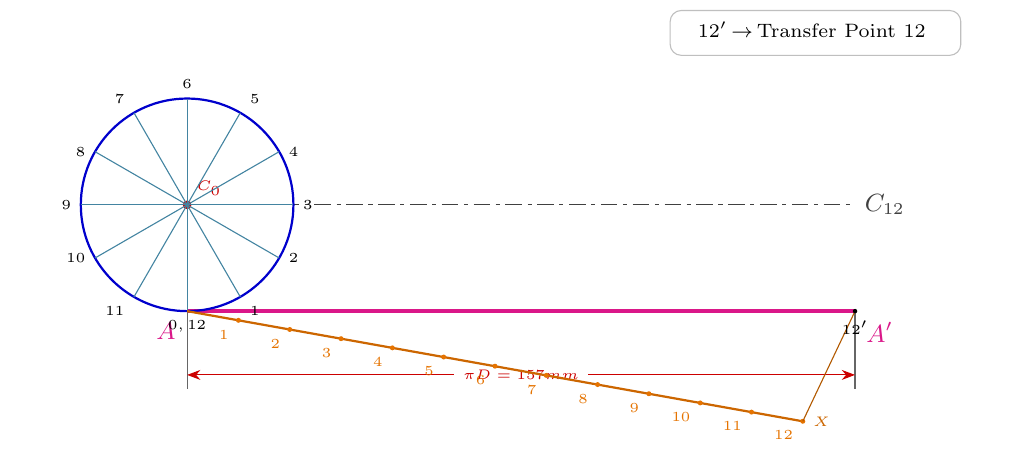
\begin{tikzpicture}[scale=0.45]
  \useasboundingbox (-4.5,-3.5) rectangle (22.5,8.0);
  \drawLegendCard{ \textbf{$12'$} & Transfer Point 12 }
  \draw[directrix line] (0,0) node[below left] {\small $A$} -- (18.85,0) node[below right] {\small $A'$};
  \draw[axis line] (0,3.0) -- (18.85,3.0) node[right] {\small $C_{12}$};
  \coordinate (C0) at (0,3.0);
  \fill[red!80!black] (C0) circle (3.5pt) node[above right, font=\tiny] {$C_0$};
  \draw[thick, blue!80!black] (C0) circle (3.0);
  \draw[thin, construction line] (0,0) -- (C0);
  \draw[thin, cyan!60!black, solid] (C0) -- (0,0);
  \draw[thin, cyan!60!black, solid] (C0) -- ++(300:3.0);
  \draw[thin, cyan!60!black, solid] (C0) -- ++(330:3.0);
  \draw[thin, cyan!60!black, solid] (C0) -- ++(0:3.0);
  \draw[thin, cyan!60!black, solid] (C0) -- ++(30:3.0);
  \draw[thin, cyan!60!black, solid] (C0) -- ++(60:3.0);
  \draw[thin, cyan!60!black, solid] (C0) -- ++(90:3.0);
  \draw[thin, cyan!60!black, solid] (C0) -- ++(120:3.0);
  \draw[thin, cyan!60!black, solid] (C0) -- ++(150:3.0);
  \draw[thin, cyan!60!black, solid] (C0) -- ++(180:3.0);
  \draw[thin, cyan!60!black, solid] (C0) -- ++(210:3.0);
  \draw[thin, cyan!60!black, solid] (C0) -- ++(240:3.0);
  \node[below, font=\tiny] at (0,0) {$0, 12$};
  \node[below right, font=\tiny] at (1.5,0.40) {1};
  \node[right, font=\tiny] at (2.598,1.5) {2};
  \node[right, font=\tiny] at (3.0,3.0) {3};
  \node[right, font=\tiny] at (2.598,4.5) {4};
  \node[above right, font=\tiny] at (1.5,5.598) {5};
  \node[above, font=\tiny] at (0,6.0) {6};
  \node[above left, font=\tiny] at (-1.5,5.598) {7};
  \node[left, font=\tiny] at (-2.598,4.5) {8};
  \node[left, font=\tiny] at (-3.0,3.0) {9};
  \node[left, font=\tiny] at (-2.598,1.5) {10};
  \node[below left, font=\tiny] at (-1.5,0.40) {11};
  \draw[dimension extension] (0,0) -- (0,-2.2);
  \draw[dimension extension] (18.85,0) -- (18.85,-2.2);
  \draw[<->, red!80!black, thin] (0,-1.8) -- (18.85,-1.8) node[midway, fill=white] {\tiny $\pi D = 157\text{ mm}$};
  \draw[thick, orange!80!black] (0,0) -- (17.38,-3.11) node[right, font=\tiny] {$X$};
  \foreach \i in {1,2,...,12} {
    \coordinate (a\i) at ({\i*1.448}, {-\i*0.259});
    \fill[orange!90!black] (a\i) circle (2.0pt);
    \node[below left, font=\tiny, orange!90!black] at (a\i) {\i};
  }
  \coordinate (a12) at ({12*1.448}, {-12*0.259});
  \draw[thin, orange!70!black, solid] (a12) -- (18.85, 0);
  \fill[black] (18.85, 0) circle (1.8pt);
  \node[below, font=\tiny] at (18.85, 0) {$12'$};
\end{tikzpicture}
\end{frame}

\begin{frame}{Step 3: Divide Directing Line - Transfer Point 11'}
\centering
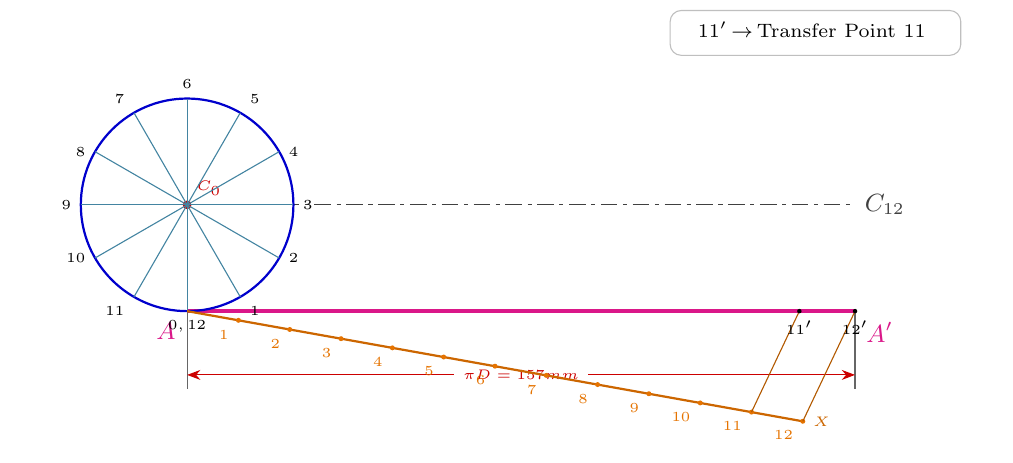
\begin{tikzpicture}[scale=0.45]
  \useasboundingbox (-4.5,-3.5) rectangle (22.5,8.0);
  \drawLegendCard{ \textbf{$11'$} & Transfer Point 11 }
  \draw[directrix line] (0,0) node[below left] {\small $A$} -- (18.85,0) node[below right] {\small $A'$};
  \draw[axis line] (0,3.0) -- (18.85,3.0) node[right] {\small $C_{12}$};
  \coordinate (C0) at (0,3.0);
  \fill[red!80!black] (C0) circle (3.5pt) node[above right, font=\tiny] {$C_0$};
  \draw[thick, blue!80!black] (C0) circle (3.0);
  \draw[thin, construction line] (0,0) -- (C0);
  \draw[thin, cyan!60!black, solid] (C0) -- (0,0);
  \draw[thin, cyan!60!black, solid] (C0) -- ++(300:3.0);
  \draw[thin, cyan!60!black, solid] (C0) -- ++(330:3.0);
  \draw[thin, cyan!60!black, solid] (C0) -- ++(0:3.0);
  \draw[thin, cyan!60!black, solid] (C0) -- ++(30:3.0);
  \draw[thin, cyan!60!black, solid] (C0) -- ++(60:3.0);
  \draw[thin, cyan!60!black, solid] (C0) -- ++(90:3.0);
  \draw[thin, cyan!60!black, solid] (C0) -- ++(120:3.0);
  \draw[thin, cyan!60!black, solid] (C0) -- ++(150:3.0);
  \draw[thin, cyan!60!black, solid] (C0) -- ++(180:3.0);
  \draw[thin, cyan!60!black, solid] (C0) -- ++(210:3.0);
  \draw[thin, cyan!60!black, solid] (C0) -- ++(240:3.0);
  \node[below, font=\tiny] at (0,0) {$0, 12$};
  \node[below right, font=\tiny] at (1.5,0.40) {1};
  \node[right, font=\tiny] at (2.598,1.5) {2};
  \node[right, font=\tiny] at (3.0,3.0) {3};
  \node[right, font=\tiny] at (2.598,4.5) {4};
  \node[above right, font=\tiny] at (1.5,5.598) {5};
  \node[above, font=\tiny] at (0,6.0) {6};
  \node[above left, font=\tiny] at (-1.5,5.598) {7};
  \node[left, font=\tiny] at (-2.598,4.5) {8};
  \node[left, font=\tiny] at (-3.0,3.0) {9};
  \node[left, font=\tiny] at (-2.598,1.5) {10};
  \node[below left, font=\tiny] at (-1.5,0.40) {11};
  \draw[dimension extension] (0,0) -- (0,-2.2);
  \draw[dimension extension] (18.85,0) -- (18.85,-2.2);
  \draw[<->, red!80!black, thin] (0,-1.8) -- (18.85,-1.8) node[midway, fill=white] {\tiny $\pi D = 157\text{ mm}$};
  \draw[thick, orange!80!black] (0,0) -- (17.38,-3.11) node[right, font=\tiny] {$X$};
  \foreach \i in {1,2,...,12} {
    \coordinate (a\i) at ({\i*1.448}, {-\i*0.259});
    \fill[orange!90!black] (a\i) circle (2.0pt);
    \node[below left, font=\tiny, orange!90!black] at (a\i) {\i};
  }
  \coordinate (a12) at ({12*1.448}, {-12*0.259});
  \draw[thin, orange!70!black, solid] (a12) -- (18.85, 0);
  \fill[black] (18.85, 0) circle (1.8pt);
  \node[below, font=\tiny] at (18.85, 0) {$12'$};
  \coordinate (a11) at ({11*1.448}, {-11*0.259});
  \draw[thin, orange!70!black, solid] (a11) -- ({11*1.5708}, 0);
  \fill[black] ({11*1.5708}, 0) circle (1.8pt);
  \node[below, font=\tiny] at ({11*1.5708}, 0) {$11'$};
\end{tikzpicture}
\end{frame}

\begin{frame}{Step 3: Divide Directing Line - Transfer Point 10'}
\centering
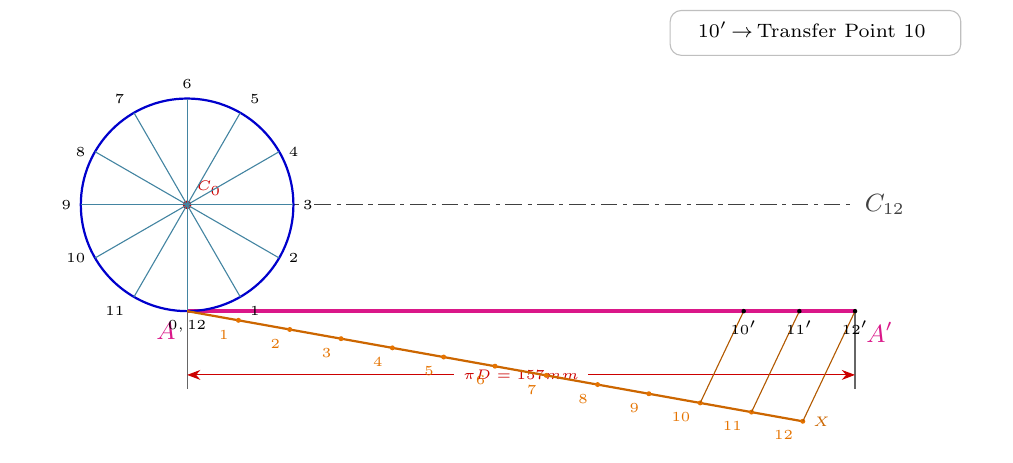
\begin{tikzpicture}[scale=0.45]
  \useasboundingbox (-4.5,-3.5) rectangle (22.5,8.0);
  \drawLegendCard{ \textbf{$10'$} & Transfer Point 10 }
  \draw[directrix line] (0,0) node[below left] {\small $A$} -- (18.85,0) node[below right] {\small $A'$};
  \draw[axis line] (0,3.0) -- (18.85,3.0) node[right] {\small $C_{12}$};
  \coordinate (C0) at (0,3.0);
  \fill[red!80!black] (C0) circle (3.5pt) node[above right, font=\tiny] {$C_0$};
  \draw[thick, blue!80!black] (C0) circle (3.0);
  \draw[thin, construction line] (0,0) -- (C0);
  \draw[thin, cyan!60!black, solid] (C0) -- (0,0);
  \draw[thin, cyan!60!black, solid] (C0) -- ++(300:3.0);
  \draw[thin, cyan!60!black, solid] (C0) -- ++(330:3.0);
  \draw[thin, cyan!60!black, solid] (C0) -- ++(0:3.0);
  \draw[thin, cyan!60!black, solid] (C0) -- ++(30:3.0);
  \draw[thin, cyan!60!black, solid] (C0) -- ++(60:3.0);
  \draw[thin, cyan!60!black, solid] (C0) -- ++(90:3.0);
  \draw[thin, cyan!60!black, solid] (C0) -- ++(120:3.0);
  \draw[thin, cyan!60!black, solid] (C0) -- ++(150:3.0);
  \draw[thin, cyan!60!black, solid] (C0) -- ++(180:3.0);
  \draw[thin, cyan!60!black, solid] (C0) -- ++(210:3.0);
  \draw[thin, cyan!60!black, solid] (C0) -- ++(240:3.0);
  \node[below, font=\tiny] at (0,0) {$0, 12$};
  \node[below right, font=\tiny] at (1.5,0.40) {1};
  \node[right, font=\tiny] at (2.598,1.5) {2};
  \node[right, font=\tiny] at (3.0,3.0) {3};
  \node[right, font=\tiny] at (2.598,4.5) {4};
  \node[above right, font=\tiny] at (1.5,5.598) {5};
  \node[above, font=\tiny] at (0,6.0) {6};
  \node[above left, font=\tiny] at (-1.5,5.598) {7};
  \node[left, font=\tiny] at (-2.598,4.5) {8};
  \node[left, font=\tiny] at (-3.0,3.0) {9};
  \node[left, font=\tiny] at (-2.598,1.5) {10};
  \node[below left, font=\tiny] at (-1.5,0.40) {11};
  \draw[dimension extension] (0,0) -- (0,-2.2);
  \draw[dimension extension] (18.85,0) -- (18.85,-2.2);
  \draw[<->, red!80!black, thin] (0,-1.8) -- (18.85,-1.8) node[midway, fill=white] {\tiny $\pi D = 157\text{ mm}$};
  \draw[thick, orange!80!black] (0,0) -- (17.38,-3.11) node[right, font=\tiny] {$X$};
  \foreach \i in {1,2,...,12} {
    \coordinate (a\i) at ({\i*1.448}, {-\i*0.259});
    \fill[orange!90!black] (a\i) circle (2.0pt);
    \node[below left, font=\tiny, orange!90!black] at (a\i) {\i};
  }
  \coordinate (a12) at ({12*1.448}, {-12*0.259});
  \draw[thin, orange!70!black, solid] (a12) -- (18.85, 0);
  \fill[black] (18.85, 0) circle (1.8pt);
  \node[below, font=\tiny] at (18.85, 0) {$12'$};
  \coordinate (a11) at ({11*1.448}, {-11*0.259});
  \draw[thin, orange!70!black, solid] (a11) -- ({11*1.5708}, 0);
  \fill[black] ({11*1.5708}, 0) circle (1.8pt);
  \node[below, font=\tiny] at ({11*1.5708}, 0) {$11'$};
  \coordinate (a10) at ({10*1.448}, {-10*0.259});
  \draw[thin, orange!70!black, solid] (a10) -- ({10*1.5708}, 0);
  \fill[black] ({10*1.5708}, 0) circle (1.8pt);
  \node[below, font=\tiny] at ({10*1.5708}, 0) {$10'$};
\end{tikzpicture}
\end{frame}

\begin{frame}{Step 3: Divide Directing Line - Transfer Point 9'}
\centering
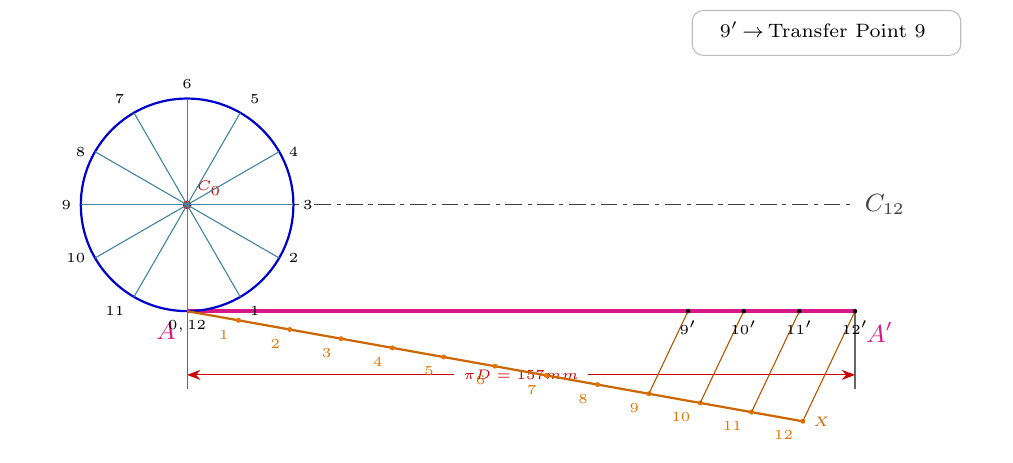
\begin{tikzpicture}[scale=0.45]
  \useasboundingbox (-4.5,-3.5) rectangle (22.5,8.0);
  \drawLegendCard{ \textbf{$9'$} & Transfer Point 9 }
  \draw[directrix line] (0,0) node[below left] {\small $A$} -- (18.85,0) node[below right] {\small $A'$};
  \draw[axis line] (0,3.0) -- (18.85,3.0) node[right] {\small $C_{12}$};
  \coordinate (C0) at (0,3.0);
  \fill[red!80!black] (C0) circle (3.5pt) node[above right, font=\tiny] {$C_0$};
  \draw[thick, blue!80!black] (C0) circle (3.0);
  \draw[thin, construction line] (0,0) -- (C0);
  \draw[thin, cyan!60!black, solid] (C0) -- (0,0);
  \draw[thin, cyan!60!black, solid] (C0) -- ++(300:3.0);
  \draw[thin, cyan!60!black, solid] (C0) -- ++(330:3.0);
  \draw[thin, cyan!60!black, solid] (C0) -- ++(0:3.0);
  \draw[thin, cyan!60!black, solid] (C0) -- ++(30:3.0);
  \draw[thin, cyan!60!black, solid] (C0) -- ++(60:3.0);
  \draw[thin, cyan!60!black, solid] (C0) -- ++(90:3.0);
  \draw[thin, cyan!60!black, solid] (C0) -- ++(120:3.0);
  \draw[thin, cyan!60!black, solid] (C0) -- ++(150:3.0);
  \draw[thin, cyan!60!black, solid] (C0) -- ++(180:3.0);
  \draw[thin, cyan!60!black, solid] (C0) -- ++(210:3.0);
  \draw[thin, cyan!60!black, solid] (C0) -- ++(240:3.0);
  \node[below, font=\tiny] at (0,0) {$0, 12$};
  \node[below right, font=\tiny] at (1.5,0.40) {1};
  \node[right, font=\tiny] at (2.598,1.5) {2};
  \node[right, font=\tiny] at (3.0,3.0) {3};
  \node[right, font=\tiny] at (2.598,4.5) {4};
  \node[above right, font=\tiny] at (1.5,5.598) {5};
  \node[above, font=\tiny] at (0,6.0) {6};
  \node[above left, font=\tiny] at (-1.5,5.598) {7};
  \node[left, font=\tiny] at (-2.598,4.5) {8};
  \node[left, font=\tiny] at (-3.0,3.0) {9};
  \node[left, font=\tiny] at (-2.598,1.5) {10};
  \node[below left, font=\tiny] at (-1.5,0.40) {11};
  \draw[dimension extension] (0,0) -- (0,-2.2);
  \draw[dimension extension] (18.85,0) -- (18.85,-2.2);
  \draw[<->, red!80!black, thin] (0,-1.8) -- (18.85,-1.8) node[midway, fill=white] {\tiny $\pi D = 157\text{ mm}$};
  \draw[thick, orange!80!black] (0,0) -- (17.38,-3.11) node[right, font=\tiny] {$X$};
  \foreach \i in {1,2,...,12} {
    \coordinate (a\i) at ({\i*1.448}, {-\i*0.259});
    \fill[orange!90!black] (a\i) circle (2.0pt);
    \node[below left, font=\tiny, orange!90!black] at (a\i) {\i};
  }
  \coordinate (a12) at ({12*1.448}, {-12*0.259});
  \draw[thin, orange!70!black, solid] (a12) -- (18.85, 0);
  \fill[black] (18.85, 0) circle (1.8pt);
  \node[below, font=\tiny] at (18.85, 0) {$12'$};
  \coordinate (a11) at ({11*1.448}, {-11*0.259});
  \draw[thin, orange!70!black, solid] (a11) -- ({11*1.5708}, 0);
  \fill[black] ({11*1.5708}, 0) circle (1.8pt);
  \node[below, font=\tiny] at ({11*1.5708}, 0) {$11'$};
  \coordinate (a10) at ({10*1.448}, {-10*0.259});
  \draw[thin, orange!70!black, solid] (a10) -- ({10*1.5708}, 0);
  \fill[black] ({10*1.5708}, 0) circle (1.8pt);
  \node[below, font=\tiny] at ({10*1.5708}, 0) {$10'$};
  \coordinate (a9) at ({9*1.448}, {-9*0.259});
  \draw[thin, orange!70!black, solid] (a9) -- ({9*1.5708}, 0);
  \fill[black] ({9*1.5708}, 0) circle (1.8pt);
  \node[below, font=\tiny] at ({9*1.5708}, 0) {$9'$};
\end{tikzpicture}
\end{frame}

\begin{frame}{Step 3: Divide Directing Line - Transfer Point 8'}
\centering
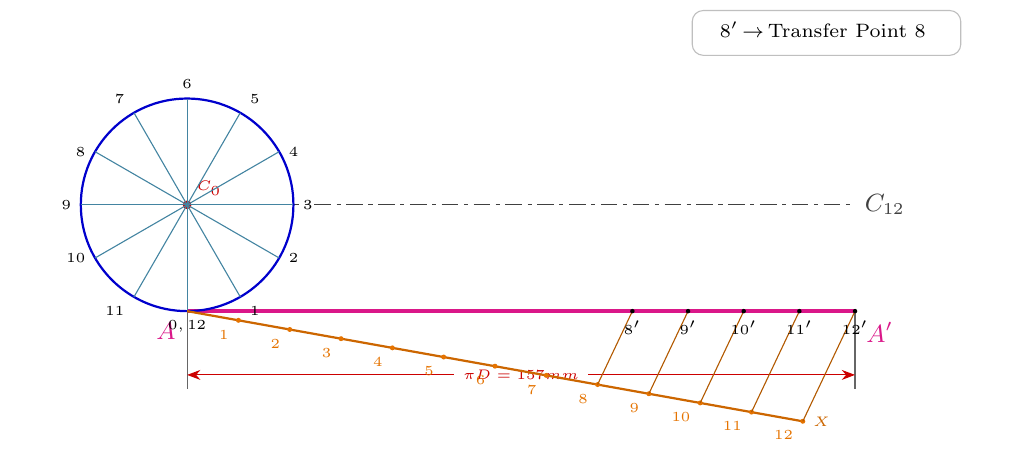
\begin{tikzpicture}[scale=0.45]
  \useasboundingbox (-4.5,-3.5) rectangle (22.5,8.0);
  \drawLegendCard{ \textbf{$8'$} & Transfer Point 8 }
  \draw[directrix line] (0,0) node[below left] {\small $A$} -- (18.85,0) node[below right] {\small $A'$};
  \draw[axis line] (0,3.0) -- (18.85,3.0) node[right] {\small $C_{12}$};
  \coordinate (C0) at (0,3.0);
  \fill[red!80!black] (C0) circle (3.5pt) node[above right, font=\tiny] {$C_0$};
  \draw[thick, blue!80!black] (C0) circle (3.0);
  \draw[thin, construction line] (0,0) -- (C0);
  \draw[thin, cyan!60!black, solid] (C0) -- (0,0);
  \draw[thin, cyan!60!black, solid] (C0) -- ++(300:3.0);
  \draw[thin, cyan!60!black, solid] (C0) -- ++(330:3.0);
  \draw[thin, cyan!60!black, solid] (C0) -- ++(0:3.0);
  \draw[thin, cyan!60!black, solid] (C0) -- ++(30:3.0);
  \draw[thin, cyan!60!black, solid] (C0) -- ++(60:3.0);
  \draw[thin, cyan!60!black, solid] (C0) -- ++(90:3.0);
  \draw[thin, cyan!60!black, solid] (C0) -- ++(120:3.0);
  \draw[thin, cyan!60!black, solid] (C0) -- ++(150:3.0);
  \draw[thin, cyan!60!black, solid] (C0) -- ++(180:3.0);
  \draw[thin, cyan!60!black, solid] (C0) -- ++(210:3.0);
  \draw[thin, cyan!60!black, solid] (C0) -- ++(240:3.0);
  \node[below, font=\tiny] at (0,0) {$0, 12$};
  \node[below right, font=\tiny] at (1.5,0.40) {1};
  \node[right, font=\tiny] at (2.598,1.5) {2};
  \node[right, font=\tiny] at (3.0,3.0) {3};
  \node[right, font=\tiny] at (2.598,4.5) {4};
  \node[above right, font=\tiny] at (1.5,5.598) {5};
  \node[above, font=\tiny] at (0,6.0) {6};
  \node[above left, font=\tiny] at (-1.5,5.598) {7};
  \node[left, font=\tiny] at (-2.598,4.5) {8};
  \node[left, font=\tiny] at (-3.0,3.0) {9};
  \node[left, font=\tiny] at (-2.598,1.5) {10};
  \node[below left, font=\tiny] at (-1.5,0.40) {11};
  \draw[dimension extension] (0,0) -- (0,-2.2);
  \draw[dimension extension] (18.85,0) -- (18.85,-2.2);
  \draw[<->, red!80!black, thin] (0,-1.8) -- (18.85,-1.8) node[midway, fill=white] {\tiny $\pi D = 157\text{ mm}$};
  \draw[thick, orange!80!black] (0,0) -- (17.38,-3.11) node[right, font=\tiny] {$X$};
  \foreach \i in {1,2,...,12} {
    \coordinate (a\i) at ({\i*1.448}, {-\i*0.259});
    \fill[orange!90!black] (a\i) circle (2.0pt);
    \node[below left, font=\tiny, orange!90!black] at (a\i) {\i};
  }
  \coordinate (a12) at ({12*1.448}, {-12*0.259});
  \draw[thin, orange!70!black, solid] (a12) -- (18.85, 0);
  \fill[black] (18.85, 0) circle (1.8pt);
  \node[below, font=\tiny] at (18.85, 0) {$12'$};
  \coordinate (a11) at ({11*1.448}, {-11*0.259});
  \draw[thin, orange!70!black, solid] (a11) -- ({11*1.5708}, 0);
  \fill[black] ({11*1.5708}, 0) circle (1.8pt);
  \node[below, font=\tiny] at ({11*1.5708}, 0) {$11'$};
  \coordinate (a10) at ({10*1.448}, {-10*0.259});
  \draw[thin, orange!70!black, solid] (a10) -- ({10*1.5708}, 0);
  \fill[black] ({10*1.5708}, 0) circle (1.8pt);
  \node[below, font=\tiny] at ({10*1.5708}, 0) {$10'$};
  \coordinate (a9) at ({9*1.448}, {-9*0.259});
  \draw[thin, orange!70!black, solid] (a9) -- ({9*1.5708}, 0);
  \fill[black] ({9*1.5708}, 0) circle (1.8pt);
  \node[below, font=\tiny] at ({9*1.5708}, 0) {$9'$};
  \coordinate (a8) at ({8*1.448}, {-8*0.259});
  \draw[thin, orange!70!black, solid] (a8) -- ({8*1.5708}, 0);
  \fill[black] ({8*1.5708}, 0) circle (1.8pt);
  \node[below, font=\tiny] at ({8*1.5708}, 0) {$8'$};
\end{tikzpicture}
\end{frame}

\begin{frame}{Step 3: Divide Directing Line - Transfer Point 7'}
\centering
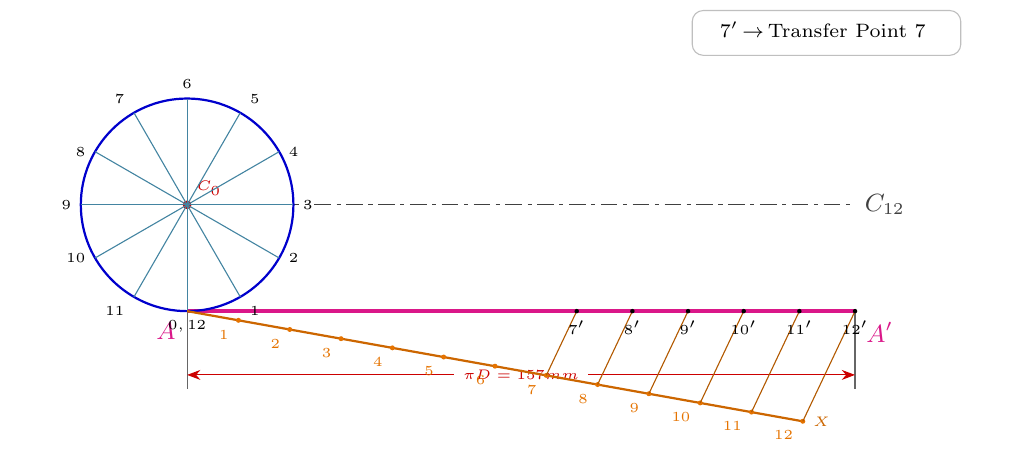
\begin{tikzpicture}[scale=0.45]
  \useasboundingbox (-4.5,-3.5) rectangle (22.5,8.0);
  \drawLegendCard{ \textbf{$7'$} & Transfer Point 7 }
  \draw[directrix line] (0,0) node[below left] {\small $A$} -- (18.85,0) node[below right] {\small $A'$};
  \draw[axis line] (0,3.0) -- (18.85,3.0) node[right] {\small $C_{12}$};
  \coordinate (C0) at (0,3.0);
  \fill[red!80!black] (C0) circle (3.5pt) node[above right, font=\tiny] {$C_0$};
  \draw[thick, blue!80!black] (C0) circle (3.0);
  \draw[thin, construction line] (0,0) -- (C0);
  \draw[thin, cyan!60!black, solid] (C0) -- (0,0);
  \draw[thin, cyan!60!black, solid] (C0) -- ++(300:3.0);
  \draw[thin, cyan!60!black, solid] (C0) -- ++(330:3.0);
  \draw[thin, cyan!60!black, solid] (C0) -- ++(0:3.0);
  \draw[thin, cyan!60!black, solid] (C0) -- ++(30:3.0);
  \draw[thin, cyan!60!black, solid] (C0) -- ++(60:3.0);
  \draw[thin, cyan!60!black, solid] (C0) -- ++(90:3.0);
  \draw[thin, cyan!60!black, solid] (C0) -- ++(120:3.0);
  \draw[thin, cyan!60!black, solid] (C0) -- ++(150:3.0);
  \draw[thin, cyan!60!black, solid] (C0) -- ++(180:3.0);
  \draw[thin, cyan!60!black, solid] (C0) -- ++(210:3.0);
  \draw[thin, cyan!60!black, solid] (C0) -- ++(240:3.0);
  \node[below, font=\tiny] at (0,0) {$0, 12$};
  \node[below right, font=\tiny] at (1.5,0.40) {1};
  \node[right, font=\tiny] at (2.598,1.5) {2};
  \node[right, font=\tiny] at (3.0,3.0) {3};
  \node[right, font=\tiny] at (2.598,4.5) {4};
  \node[above right, font=\tiny] at (1.5,5.598) {5};
  \node[above, font=\tiny] at (0,6.0) {6};
  \node[above left, font=\tiny] at (-1.5,5.598) {7};
  \node[left, font=\tiny] at (-2.598,4.5) {8};
  \node[left, font=\tiny] at (-3.0,3.0) {9};
  \node[left, font=\tiny] at (-2.598,1.5) {10};
  \node[below left, font=\tiny] at (-1.5,0.40) {11};
  \draw[dimension extension] (0,0) -- (0,-2.2);
  \draw[dimension extension] (18.85,0) -- (18.85,-2.2);
  \draw[<->, red!80!black, thin] (0,-1.8) -- (18.85,-1.8) node[midway, fill=white] {\tiny $\pi D = 157\text{ mm}$};
  \draw[thick, orange!80!black] (0,0) -- (17.38,-3.11) node[right, font=\tiny] {$X$};
  \foreach \i in {1,2,...,12} {
    \coordinate (a\i) at ({\i*1.448}, {-\i*0.259});
    \fill[orange!90!black] (a\i) circle (2.0pt);
    \node[below left, font=\tiny, orange!90!black] at (a\i) {\i};
  }
  \coordinate (a12) at ({12*1.448}, {-12*0.259});
  \draw[thin, orange!70!black, solid] (a12) -- (18.85, 0);
  \fill[black] (18.85, 0) circle (1.8pt);
  \node[below, font=\tiny] at (18.85, 0) {$12'$};
  \coordinate (a11) at ({11*1.448}, {-11*0.259});
  \draw[thin, orange!70!black, solid] (a11) -- ({11*1.5708}, 0);
  \fill[black] ({11*1.5708}, 0) circle (1.8pt);
  \node[below, font=\tiny] at ({11*1.5708}, 0) {$11'$};
  \coordinate (a10) at ({10*1.448}, {-10*0.259});
  \draw[thin, orange!70!black, solid] (a10) -- ({10*1.5708}, 0);
  \fill[black] ({10*1.5708}, 0) circle (1.8pt);
  \node[below, font=\tiny] at ({10*1.5708}, 0) {$10'$};
  \coordinate (a9) at ({9*1.448}, {-9*0.259});
  \draw[thin, orange!70!black, solid] (a9) -- ({9*1.5708}, 0);
  \fill[black] ({9*1.5708}, 0) circle (1.8pt);
  \node[below, font=\tiny] at ({9*1.5708}, 0) {$9'$};
  \coordinate (a8) at ({8*1.448}, {-8*0.259});
  \draw[thin, orange!70!black, solid] (a8) -- ({8*1.5708}, 0);
  \fill[black] ({8*1.5708}, 0) circle (1.8pt);
  \node[below, font=\tiny] at ({8*1.5708}, 0) {$8'$};
  \coordinate (a7) at ({7*1.448}, {-7*0.259});
  \draw[thin, orange!70!black, solid] (a7) -- ({7*1.5708}, 0);
  \fill[black] ({7*1.5708}, 0) circle (1.8pt);
  \node[below, font=\tiny] at ({7*1.5708}, 0) {$7'$};
\end{tikzpicture}
\end{frame}

\begin{frame}{Step 3: Divide Directing Line - Transfer Point 6'}
\centering
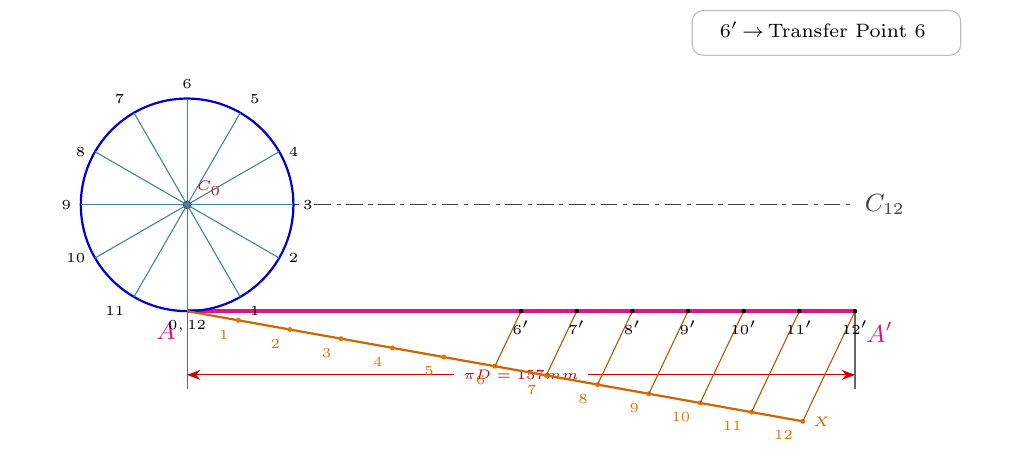
\begin{tikzpicture}[scale=0.45]
  \useasboundingbox (-4.5,-3.5) rectangle (22.5,8.0);
  \drawLegendCard{ \textbf{$6'$} & Transfer Point 6 }
  \draw[directrix line] (0,0) node[below left] {\small $A$} -- (18.85,0) node[below right] {\small $A'$};
  \draw[axis line] (0,3.0) -- (18.85,3.0) node[right] {\small $C_{12}$};
  \coordinate (C0) at (0,3.0);
  \fill[red!80!black] (C0) circle (3.5pt) node[above right, font=\tiny] {$C_0$};
  \draw[thick, blue!80!black] (C0) circle (3.0);
  \draw[thin, construction line] (0,0) -- (C0);
  \draw[thin, cyan!60!black, solid] (C0) -- (0,0);
  \draw[thin, cyan!60!black, solid] (C0) -- ++(300:3.0);
  \draw[thin, cyan!60!black, solid] (C0) -- ++(330:3.0);
  \draw[thin, cyan!60!black, solid] (C0) -- ++(0:3.0);
  \draw[thin, cyan!60!black, solid] (C0) -- ++(30:3.0);
  \draw[thin, cyan!60!black, solid] (C0) -- ++(60:3.0);
  \draw[thin, cyan!60!black, solid] (C0) -- ++(90:3.0);
  \draw[thin, cyan!60!black, solid] (C0) -- ++(120:3.0);
  \draw[thin, cyan!60!black, solid] (C0) -- ++(150:3.0);
  \draw[thin, cyan!60!black, solid] (C0) -- ++(180:3.0);
  \draw[thin, cyan!60!black, solid] (C0) -- ++(210:3.0);
  \draw[thin, cyan!60!black, solid] (C0) -- ++(240:3.0);
  \node[below, font=\tiny] at (0,0) {$0, 12$};
  \node[below right, font=\tiny] at (1.5,0.40) {1};
  \node[right, font=\tiny] at (2.598,1.5) {2};
  \node[right, font=\tiny] at (3.0,3.0) {3};
  \node[right, font=\tiny] at (2.598,4.5) {4};
  \node[above right, font=\tiny] at (1.5,5.598) {5};
  \node[above, font=\tiny] at (0,6.0) {6};
  \node[above left, font=\tiny] at (-1.5,5.598) {7};
  \node[left, font=\tiny] at (-2.598,4.5) {8};
  \node[left, font=\tiny] at (-3.0,3.0) {9};
  \node[left, font=\tiny] at (-2.598,1.5) {10};
  \node[below left, font=\tiny] at (-1.5,0.40) {11};
  \draw[dimension extension] (0,0) -- (0,-2.2);
  \draw[dimension extension] (18.85,0) -- (18.85,-2.2);
  \draw[<->, red!80!black, thin] (0,-1.8) -- (18.85,-1.8) node[midway, fill=white] {\tiny $\pi D = 157\text{ mm}$};
  \draw[thick, orange!80!black] (0,0) -- (17.38,-3.11) node[right, font=\tiny] {$X$};
  \foreach \i in {1,2,...,12} {
    \coordinate (a\i) at ({\i*1.448}, {-\i*0.259});
    \fill[orange!90!black] (a\i) circle (2.0pt);
    \node[below left, font=\tiny, orange!90!black] at (a\i) {\i};
  }
  \coordinate (a12) at ({12*1.448}, {-12*0.259});
  \draw[thin, orange!70!black, solid] (a12) -- (18.85, 0);
  \fill[black] (18.85, 0) circle (1.8pt);
  \node[below, font=\tiny] at (18.85, 0) {$12'$};
  \coordinate (a11) at ({11*1.448}, {-11*0.259});
  \draw[thin, orange!70!black, solid] (a11) -- ({11*1.5708}, 0);
  \fill[black] ({11*1.5708}, 0) circle (1.8pt);
  \node[below, font=\tiny] at ({11*1.5708}, 0) {$11'$};
  \coordinate (a10) at ({10*1.448}, {-10*0.259});
  \draw[thin, orange!70!black, solid] (a10) -- ({10*1.5708}, 0);
  \fill[black] ({10*1.5708}, 0) circle (1.8pt);
  \node[below, font=\tiny] at ({10*1.5708}, 0) {$10'$};
  \coordinate (a9) at ({9*1.448}, {-9*0.259});
  \draw[thin, orange!70!black, solid] (a9) -- ({9*1.5708}, 0);
  \fill[black] ({9*1.5708}, 0) circle (1.8pt);
  \node[below, font=\tiny] at ({9*1.5708}, 0) {$9'$};
  \coordinate (a8) at ({8*1.448}, {-8*0.259});
  \draw[thin, orange!70!black, solid] (a8) -- ({8*1.5708}, 0);
  \fill[black] ({8*1.5708}, 0) circle (1.8pt);
  \node[below, font=\tiny] at ({8*1.5708}, 0) {$8'$};
  \coordinate (a7) at ({7*1.448}, {-7*0.259});
  \draw[thin, orange!70!black, solid] (a7) -- ({7*1.5708}, 0);
  \fill[black] ({7*1.5708}, 0) circle (1.8pt);
  \node[below, font=\tiny] at ({7*1.5708}, 0) {$7'$};
  \coordinate (a6) at ({6*1.448}, {-6*0.259});
  \draw[thin, orange!70!black, solid] (a6) -- ({6*1.5708}, 0);
  \fill[black] ({6*1.5708}, 0) circle (1.8pt);
  \node[below, font=\tiny] at ({6*1.5708}, 0) {$6'$};
\end{tikzpicture}
\end{frame}

\begin{frame}{Step 3: Divide Directing Line - Transfer Point 5'}
\centering
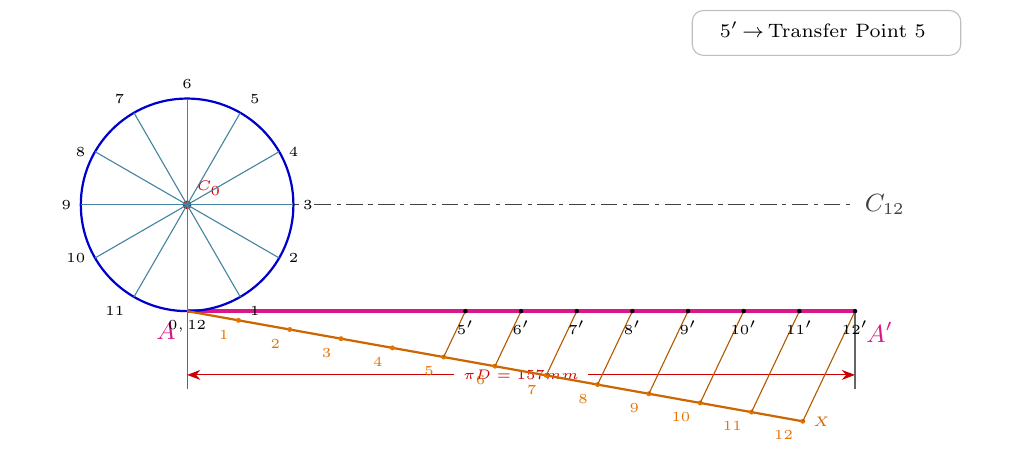
\begin{tikzpicture}[scale=0.45]
  \useasboundingbox (-4.5,-3.5) rectangle (22.5,8.0);
  \drawLegendCard{ \textbf{$5'$} & Transfer Point 5 }
  \draw[directrix line] (0,0) node[below left] {\small $A$} -- (18.85,0) node[below right] {\small $A'$};
  \draw[axis line] (0,3.0) -- (18.85,3.0) node[right] {\small $C_{12}$};
  \coordinate (C0) at (0,3.0);
  \fill[red!80!black] (C0) circle (3.5pt) node[above right, font=\tiny] {$C_0$};
  \draw[thick, blue!80!black] (C0) circle (3.0);
  \draw[thin, construction line] (0,0) -- (C0);
  \draw[thin, cyan!60!black, solid] (C0) -- (0,0);
  \draw[thin, cyan!60!black, solid] (C0) -- ++(300:3.0);
  \draw[thin, cyan!60!black, solid] (C0) -- ++(330:3.0);
  \draw[thin, cyan!60!black, solid] (C0) -- ++(0:3.0);
  \draw[thin, cyan!60!black, solid] (C0) -- ++(30:3.0);
  \draw[thin, cyan!60!black, solid] (C0) -- ++(60:3.0);
  \draw[thin, cyan!60!black, solid] (C0) -- ++(90:3.0);
  \draw[thin, cyan!60!black, solid] (C0) -- ++(120:3.0);
  \draw[thin, cyan!60!black, solid] (C0) -- ++(150:3.0);
  \draw[thin, cyan!60!black, solid] (C0) -- ++(180:3.0);
  \draw[thin, cyan!60!black, solid] (C0) -- ++(210:3.0);
  \draw[thin, cyan!60!black, solid] (C0) -- ++(240:3.0);
  \node[below, font=\tiny] at (0,0) {$0, 12$};
  \node[below right, font=\tiny] at (1.5,0.40) {1};
  \node[right, font=\tiny] at (2.598,1.5) {2};
  \node[right, font=\tiny] at (3.0,3.0) {3};
  \node[right, font=\tiny] at (2.598,4.5) {4};
  \node[above right, font=\tiny] at (1.5,5.598) {5};
  \node[above, font=\tiny] at (0,6.0) {6};
  \node[above left, font=\tiny] at (-1.5,5.598) {7};
  \node[left, font=\tiny] at (-2.598,4.5) {8};
  \node[left, font=\tiny] at (-3.0,3.0) {9};
  \node[left, font=\tiny] at (-2.598,1.5) {10};
  \node[below left, font=\tiny] at (-1.5,0.40) {11};
  \draw[dimension extension] (0,0) -- (0,-2.2);
  \draw[dimension extension] (18.85,0) -- (18.85,-2.2);
  \draw[<->, red!80!black, thin] (0,-1.8) -- (18.85,-1.8) node[midway, fill=white] {\tiny $\pi D = 157\text{ mm}$};
  \draw[thick, orange!80!black] (0,0) -- (17.38,-3.11) node[right, font=\tiny] {$X$};
  \foreach \i in {1,2,...,12} {
    \coordinate (a\i) at ({\i*1.448}, {-\i*0.259});
    \fill[orange!90!black] (a\i) circle (2.0pt);
    \node[below left, font=\tiny, orange!90!black] at (a\i) {\i};
  }
  \coordinate (a12) at ({12*1.448}, {-12*0.259});
  \draw[thin, orange!70!black, solid] (a12) -- (18.85, 0);
  \fill[black] (18.85, 0) circle (1.8pt);
  \node[below, font=\tiny] at (18.85, 0) {$12'$};
  \coordinate (a11) at ({11*1.448}, {-11*0.259});
  \draw[thin, orange!70!black, solid] (a11) -- ({11*1.5708}, 0);
  \fill[black] ({11*1.5708}, 0) circle (1.8pt);
  \node[below, font=\tiny] at ({11*1.5708}, 0) {$11'$};
  \coordinate (a10) at ({10*1.448}, {-10*0.259});
  \draw[thin, orange!70!black, solid] (a10) -- ({10*1.5708}, 0);
  \fill[black] ({10*1.5708}, 0) circle (1.8pt);
  \node[below, font=\tiny] at ({10*1.5708}, 0) {$10'$};
  \coordinate (a9) at ({9*1.448}, {-9*0.259});
  \draw[thin, orange!70!black, solid] (a9) -- ({9*1.5708}, 0);
  \fill[black] ({9*1.5708}, 0) circle (1.8pt);
  \node[below, font=\tiny] at ({9*1.5708}, 0) {$9'$};
  \coordinate (a8) at ({8*1.448}, {-8*0.259});
  \draw[thin, orange!70!black, solid] (a8) -- ({8*1.5708}, 0);
  \fill[black] ({8*1.5708}, 0) circle (1.8pt);
  \node[below, font=\tiny] at ({8*1.5708}, 0) {$8'$};
  \coordinate (a7) at ({7*1.448}, {-7*0.259});
  \draw[thin, orange!70!black, solid] (a7) -- ({7*1.5708}, 0);
  \fill[black] ({7*1.5708}, 0) circle (1.8pt);
  \node[below, font=\tiny] at ({7*1.5708}, 0) {$7'$};
  \coordinate (a6) at ({6*1.448}, {-6*0.259});
  \draw[thin, orange!70!black, solid] (a6) -- ({6*1.5708}, 0);
  \fill[black] ({6*1.5708}, 0) circle (1.8pt);
  \node[below, font=\tiny] at ({6*1.5708}, 0) {$6'$};
  \coordinate (a5) at ({5*1.448}, {-5*0.259});
  \draw[thin, orange!70!black, solid] (a5) -- ({5*1.5708}, 0);
  \fill[black] ({5*1.5708}, 0) circle (1.8pt);
  \node[below, font=\tiny] at ({5*1.5708}, 0) {$5'$};
\end{tikzpicture}
\end{frame}

\begin{frame}{Step 3: Divide Directing Line - Transfer Point 4'}
\centering
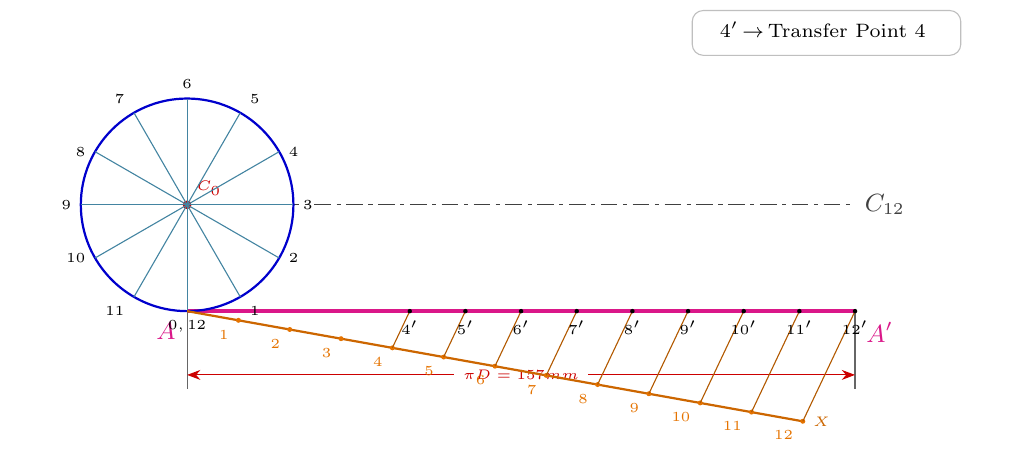
\begin{tikzpicture}[scale=0.45]
  \useasboundingbox (-4.5,-3.5) rectangle (22.5,8.0);
  \drawLegendCard{ \textbf{$4'$} & Transfer Point 4 }
  \draw[directrix line] (0,0) node[below left] {\small $A$} -- (18.85,0) node[below right] {\small $A'$};
  \draw[axis line] (0,3.0) -- (18.85,3.0) node[right] {\small $C_{12}$};
  \coordinate (C0) at (0,3.0);
  \fill[red!80!black] (C0) circle (3.5pt) node[above right, font=\tiny] {$C_0$};
  \draw[thick, blue!80!black] (C0) circle (3.0);
  \draw[thin, construction line] (0,0) -- (C0);
  \draw[thin, cyan!60!black, solid] (C0) -- (0,0);
  \draw[thin, cyan!60!black, solid] (C0) -- ++(300:3.0);
  \draw[thin, cyan!60!black, solid] (C0) -- ++(330:3.0);
  \draw[thin, cyan!60!black, solid] (C0) -- ++(0:3.0);
  \draw[thin, cyan!60!black, solid] (C0) -- ++(30:3.0);
  \draw[thin, cyan!60!black, solid] (C0) -- ++(60:3.0);
  \draw[thin, cyan!60!black, solid] (C0) -- ++(90:3.0);
  \draw[thin, cyan!60!black, solid] (C0) -- ++(120:3.0);
  \draw[thin, cyan!60!black, solid] (C0) -- ++(150:3.0);
  \draw[thin, cyan!60!black, solid] (C0) -- ++(180:3.0);
  \draw[thin, cyan!60!black, solid] (C0) -- ++(210:3.0);
  \draw[thin, cyan!60!black, solid] (C0) -- ++(240:3.0);
  \node[below, font=\tiny] at (0,0) {$0, 12$};
  \node[below right, font=\tiny] at (1.5,0.40) {1};
  \node[right, font=\tiny] at (2.598,1.5) {2};
  \node[right, font=\tiny] at (3.0,3.0) {3};
  \node[right, font=\tiny] at (2.598,4.5) {4};
  \node[above right, font=\tiny] at (1.5,5.598) {5};
  \node[above, font=\tiny] at (0,6.0) {6};
  \node[above left, font=\tiny] at (-1.5,5.598) {7};
  \node[left, font=\tiny] at (-2.598,4.5) {8};
  \node[left, font=\tiny] at (-3.0,3.0) {9};
  \node[left, font=\tiny] at (-2.598,1.5) {10};
  \node[below left, font=\tiny] at (-1.5,0.40) {11};
  \draw[dimension extension] (0,0) -- (0,-2.2);
  \draw[dimension extension] (18.85,0) -- (18.85,-2.2);
  \draw[<->, red!80!black, thin] (0,-1.8) -- (18.85,-1.8) node[midway, fill=white] {\tiny $\pi D = 157\text{ mm}$};
  \draw[thick, orange!80!black] (0,0) -- (17.38,-3.11) node[right, font=\tiny] {$X$};
  \foreach \i in {1,2,...,12} {
    \coordinate (a\i) at ({\i*1.448}, {-\i*0.259});
    \fill[orange!90!black] (a\i) circle (2.0pt);
    \node[below left, font=\tiny, orange!90!black] at (a\i) {\i};
  }
  \coordinate (a12) at ({12*1.448}, {-12*0.259});
  \draw[thin, orange!70!black, solid] (a12) -- (18.85, 0);
  \fill[black] (18.85, 0) circle (1.8pt);
  \node[below, font=\tiny] at (18.85, 0) {$12'$};
  \coordinate (a11) at ({11*1.448}, {-11*0.259});
  \draw[thin, orange!70!black, solid] (a11) -- ({11*1.5708}, 0);
  \fill[black] ({11*1.5708}, 0) circle (1.8pt);
  \node[below, font=\tiny] at ({11*1.5708}, 0) {$11'$};
  \coordinate (a10) at ({10*1.448}, {-10*0.259});
  \draw[thin, orange!70!black, solid] (a10) -- ({10*1.5708}, 0);
  \fill[black] ({10*1.5708}, 0) circle (1.8pt);
  \node[below, font=\tiny] at ({10*1.5708}, 0) {$10'$};
  \coordinate (a9) at ({9*1.448}, {-9*0.259});
  \draw[thin, orange!70!black, solid] (a9) -- ({9*1.5708}, 0);
  \fill[black] ({9*1.5708}, 0) circle (1.8pt);
  \node[below, font=\tiny] at ({9*1.5708}, 0) {$9'$};
  \coordinate (a8) at ({8*1.448}, {-8*0.259});
  \draw[thin, orange!70!black, solid] (a8) -- ({8*1.5708}, 0);
  \fill[black] ({8*1.5708}, 0) circle (1.8pt);
  \node[below, font=\tiny] at ({8*1.5708}, 0) {$8'$};
  \coordinate (a7) at ({7*1.448}, {-7*0.259});
  \draw[thin, orange!70!black, solid] (a7) -- ({7*1.5708}, 0);
  \fill[black] ({7*1.5708}, 0) circle (1.8pt);
  \node[below, font=\tiny] at ({7*1.5708}, 0) {$7'$};
  \coordinate (a6) at ({6*1.448}, {-6*0.259});
  \draw[thin, orange!70!black, solid] (a6) -- ({6*1.5708}, 0);
  \fill[black] ({6*1.5708}, 0) circle (1.8pt);
  \node[below, font=\tiny] at ({6*1.5708}, 0) {$6'$};
  \coordinate (a5) at ({5*1.448}, {-5*0.259});
  \draw[thin, orange!70!black, solid] (a5) -- ({5*1.5708}, 0);
  \fill[black] ({5*1.5708}, 0) circle (1.8pt);
  \node[below, font=\tiny] at ({5*1.5708}, 0) {$5'$};
  \coordinate (a4) at ({4*1.448}, {-4*0.259});
  \draw[thin, orange!70!black, solid] (a4) -- ({4*1.5708}, 0);
  \fill[black] ({4*1.5708}, 0) circle (1.8pt);
  \node[below, font=\tiny] at ({4*1.5708}, 0) {$4'$};
\end{tikzpicture}
\end{frame}

\begin{frame}{Step 3: Divide Directing Line - Transfer Point 3'}
\centering
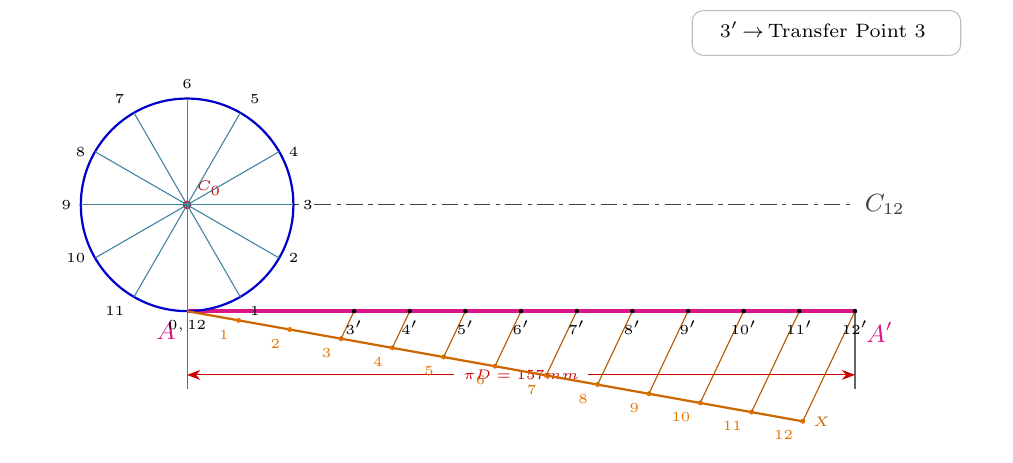
\begin{tikzpicture}[scale=0.45]
  \useasboundingbox (-4.5,-3.5) rectangle (22.5,8.0);
  \drawLegendCard{ \textbf{$3'$} & Transfer Point 3 }
  \draw[directrix line] (0,0) node[below left] {\small $A$} -- (18.85,0) node[below right] {\small $A'$};
  \draw[axis line] (0,3.0) -- (18.85,3.0) node[right] {\small $C_{12}$};
  \coordinate (C0) at (0,3.0);
  \fill[red!80!black] (C0) circle (3.5pt) node[above right, font=\tiny] {$C_0$};
  \draw[thick, blue!80!black] (C0) circle (3.0);
  \draw[thin, construction line] (0,0) -- (C0);
  \draw[thin, cyan!60!black, solid] (C0) -- (0,0);
  \draw[thin, cyan!60!black, solid] (C0) -- ++(300:3.0);
  \draw[thin, cyan!60!black, solid] (C0) -- ++(330:3.0);
  \draw[thin, cyan!60!black, solid] (C0) -- ++(0:3.0);
  \draw[thin, cyan!60!black, solid] (C0) -- ++(30:3.0);
  \draw[thin, cyan!60!black, solid] (C0) -- ++(60:3.0);
  \draw[thin, cyan!60!black, solid] (C0) -- ++(90:3.0);
  \draw[thin, cyan!60!black, solid] (C0) -- ++(120:3.0);
  \draw[thin, cyan!60!black, solid] (C0) -- ++(150:3.0);
  \draw[thin, cyan!60!black, solid] (C0) -- ++(180:3.0);
  \draw[thin, cyan!60!black, solid] (C0) -- ++(210:3.0);
  \draw[thin, cyan!60!black, solid] (C0) -- ++(240:3.0);
  \node[below, font=\tiny] at (0,0) {$0, 12$};
  \node[below right, font=\tiny] at (1.5,0.40) {1};
  \node[right, font=\tiny] at (2.598,1.5) {2};
  \node[right, font=\tiny] at (3.0,3.0) {3};
  \node[right, font=\tiny] at (2.598,4.5) {4};
  \node[above right, font=\tiny] at (1.5,5.598) {5};
  \node[above, font=\tiny] at (0,6.0) {6};
  \node[above left, font=\tiny] at (-1.5,5.598) {7};
  \node[left, font=\tiny] at (-2.598,4.5) {8};
  \node[left, font=\tiny] at (-3.0,3.0) {9};
  \node[left, font=\tiny] at (-2.598,1.5) {10};
  \node[below left, font=\tiny] at (-1.5,0.40) {11};
  \draw[dimension extension] (0,0) -- (0,-2.2);
  \draw[dimension extension] (18.85,0) -- (18.85,-2.2);
  \draw[<->, red!80!black, thin] (0,-1.8) -- (18.85,-1.8) node[midway, fill=white] {\tiny $\pi D = 157\text{ mm}$};
  \draw[thick, orange!80!black] (0,0) -- (17.38,-3.11) node[right, font=\tiny] {$X$};
  \foreach \i in {1,2,...,12} {
    \coordinate (a\i) at ({\i*1.448}, {-\i*0.259});
    \fill[orange!90!black] (a\i) circle (2.0pt);
    \node[below left, font=\tiny, orange!90!black] at (a\i) {\i};
  }
  \coordinate (a12) at ({12*1.448}, {-12*0.259});
  \draw[thin, orange!70!black, solid] (a12) -- (18.85, 0);
  \fill[black] (18.85, 0) circle (1.8pt);
  \node[below, font=\tiny] at (18.85, 0) {$12'$};
  \coordinate (a11) at ({11*1.448}, {-11*0.259});
  \draw[thin, orange!70!black, solid] (a11) -- ({11*1.5708}, 0);
  \fill[black] ({11*1.5708}, 0) circle (1.8pt);
  \node[below, font=\tiny] at ({11*1.5708}, 0) {$11'$};
  \coordinate (a10) at ({10*1.448}, {-10*0.259});
  \draw[thin, orange!70!black, solid] (a10) -- ({10*1.5708}, 0);
  \fill[black] ({10*1.5708}, 0) circle (1.8pt);
  \node[below, font=\tiny] at ({10*1.5708}, 0) {$10'$};
  \coordinate (a9) at ({9*1.448}, {-9*0.259});
  \draw[thin, orange!70!black, solid] (a9) -- ({9*1.5708}, 0);
  \fill[black] ({9*1.5708}, 0) circle (1.8pt);
  \node[below, font=\tiny] at ({9*1.5708}, 0) {$9'$};
  \coordinate (a8) at ({8*1.448}, {-8*0.259});
  \draw[thin, orange!70!black, solid] (a8) -- ({8*1.5708}, 0);
  \fill[black] ({8*1.5708}, 0) circle (1.8pt);
  \node[below, font=\tiny] at ({8*1.5708}, 0) {$8'$};
  \coordinate (a7) at ({7*1.448}, {-7*0.259});
  \draw[thin, orange!70!black, solid] (a7) -- ({7*1.5708}, 0);
  \fill[black] ({7*1.5708}, 0) circle (1.8pt);
  \node[below, font=\tiny] at ({7*1.5708}, 0) {$7'$};
  \coordinate (a6) at ({6*1.448}, {-6*0.259});
  \draw[thin, orange!70!black, solid] (a6) -- ({6*1.5708}, 0);
  \fill[black] ({6*1.5708}, 0) circle (1.8pt);
  \node[below, font=\tiny] at ({6*1.5708}, 0) {$6'$};
  \coordinate (a5) at ({5*1.448}, {-5*0.259});
  \draw[thin, orange!70!black, solid] (a5) -- ({5*1.5708}, 0);
  \fill[black] ({5*1.5708}, 0) circle (1.8pt);
  \node[below, font=\tiny] at ({5*1.5708}, 0) {$5'$};
  \coordinate (a4) at ({4*1.448}, {-4*0.259});
  \draw[thin, orange!70!black, solid] (a4) -- ({4*1.5708}, 0);
  \fill[black] ({4*1.5708}, 0) circle (1.8pt);
  \node[below, font=\tiny] at ({4*1.5708}, 0) {$4'$};
  \coordinate (a3) at ({3*1.448}, {-3*0.259});
  \draw[thin, orange!70!black, solid] (a3) -- ({3*1.5708}, 0);
  \fill[black] ({3*1.5708}, 0) circle (1.8pt);
  \node[below, font=\tiny] at ({3*1.5708}, 0) {$3'$};
\end{tikzpicture}
\end{frame}

\begin{frame}{Step 3: Divide Directing Line - Transfer Point 2'}
\centering
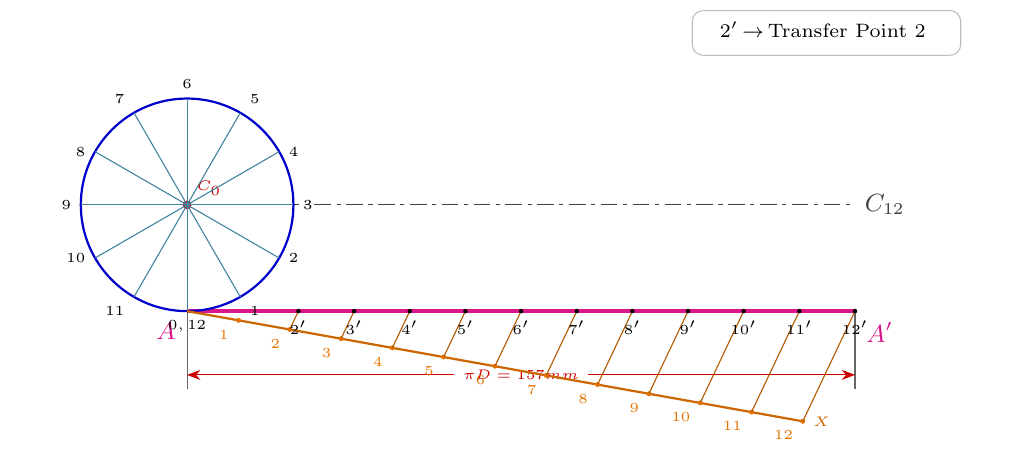
\begin{tikzpicture}[scale=0.45]
  \useasboundingbox (-4.5,-3.5) rectangle (22.5,8.0);
  \drawLegendCard{ \textbf{$2'$} & Transfer Point 2 }
  \draw[directrix line] (0,0) node[below left] {\small $A$} -- (18.85,0) node[below right] {\small $A'$};
  \draw[axis line] (0,3.0) -- (18.85,3.0) node[right] {\small $C_{12}$};
  \coordinate (C0) at (0,3.0);
  \fill[red!80!black] (C0) circle (3.5pt) node[above right, font=\tiny] {$C_0$};
  \draw[thick, blue!80!black] (C0) circle (3.0);
  \draw[thin, construction line] (0,0) -- (C0);
  \draw[thin, cyan!60!black, solid] (C0) -- (0,0);
  \draw[thin, cyan!60!black, solid] (C0) -- ++(300:3.0);
  \draw[thin, cyan!60!black, solid] (C0) -- ++(330:3.0);
  \draw[thin, cyan!60!black, solid] (C0) -- ++(0:3.0);
  \draw[thin, cyan!60!black, solid] (C0) -- ++(30:3.0);
  \draw[thin, cyan!60!black, solid] (C0) -- ++(60:3.0);
  \draw[thin, cyan!60!black, solid] (C0) -- ++(90:3.0);
  \draw[thin, cyan!60!black, solid] (C0) -- ++(120:3.0);
  \draw[thin, cyan!60!black, solid] (C0) -- ++(150:3.0);
  \draw[thin, cyan!60!black, solid] (C0) -- ++(180:3.0);
  \draw[thin, cyan!60!black, solid] (C0) -- ++(210:3.0);
  \draw[thin, cyan!60!black, solid] (C0) -- ++(240:3.0);
  \node[below, font=\tiny] at (0,0) {$0, 12$};
  \node[below right, font=\tiny] at (1.5,0.40) {1};
  \node[right, font=\tiny] at (2.598,1.5) {2};
  \node[right, font=\tiny] at (3.0,3.0) {3};
  \node[right, font=\tiny] at (2.598,4.5) {4};
  \node[above right, font=\tiny] at (1.5,5.598) {5};
  \node[above, font=\tiny] at (0,6.0) {6};
  \node[above left, font=\tiny] at (-1.5,5.598) {7};
  \node[left, font=\tiny] at (-2.598,4.5) {8};
  \node[left, font=\tiny] at (-3.0,3.0) {9};
  \node[left, font=\tiny] at (-2.598,1.5) {10};
  \node[below left, font=\tiny] at (-1.5,0.40) {11};
  \draw[dimension extension] (0,0) -- (0,-2.2);
  \draw[dimension extension] (18.85,0) -- (18.85,-2.2);
  \draw[<->, red!80!black, thin] (0,-1.8) -- (18.85,-1.8) node[midway, fill=white] {\tiny $\pi D = 157\text{ mm}$};
  \draw[thick, orange!80!black] (0,0) -- (17.38,-3.11) node[right, font=\tiny] {$X$};
  \foreach \i in {1,2,...,12} {
    \coordinate (a\i) at ({\i*1.448}, {-\i*0.259});
    \fill[orange!90!black] (a\i) circle (2.0pt);
    \node[below left, font=\tiny, orange!90!black] at (a\i) {\i};
  }
  \coordinate (a12) at ({12*1.448}, {-12*0.259});
  \draw[thin, orange!70!black, solid] (a12) -- (18.85, 0);
  \fill[black] (18.85, 0) circle (1.8pt);
  \node[below, font=\tiny] at (18.85, 0) {$12'$};
  \coordinate (a11) at ({11*1.448}, {-11*0.259});
  \draw[thin, orange!70!black, solid] (a11) -- ({11*1.5708}, 0);
  \fill[black] ({11*1.5708}, 0) circle (1.8pt);
  \node[below, font=\tiny] at ({11*1.5708}, 0) {$11'$};
  \coordinate (a10) at ({10*1.448}, {-10*0.259});
  \draw[thin, orange!70!black, solid] (a10) -- ({10*1.5708}, 0);
  \fill[black] ({10*1.5708}, 0) circle (1.8pt);
  \node[below, font=\tiny] at ({10*1.5708}, 0) {$10'$};
  \coordinate (a9) at ({9*1.448}, {-9*0.259});
  \draw[thin, orange!70!black, solid] (a9) -- ({9*1.5708}, 0);
  \fill[black] ({9*1.5708}, 0) circle (1.8pt);
  \node[below, font=\tiny] at ({9*1.5708}, 0) {$9'$};
  \coordinate (a8) at ({8*1.448}, {-8*0.259});
  \draw[thin, orange!70!black, solid] (a8) -- ({8*1.5708}, 0);
  \fill[black] ({8*1.5708}, 0) circle (1.8pt);
  \node[below, font=\tiny] at ({8*1.5708}, 0) {$8'$};
  \coordinate (a7) at ({7*1.448}, {-7*0.259});
  \draw[thin, orange!70!black, solid] (a7) -- ({7*1.5708}, 0);
  \fill[black] ({7*1.5708}, 0) circle (1.8pt);
  \node[below, font=\tiny] at ({7*1.5708}, 0) {$7'$};
  \coordinate (a6) at ({6*1.448}, {-6*0.259});
  \draw[thin, orange!70!black, solid] (a6) -- ({6*1.5708}, 0);
  \fill[black] ({6*1.5708}, 0) circle (1.8pt);
  \node[below, font=\tiny] at ({6*1.5708}, 0) {$6'$};
  \coordinate (a5) at ({5*1.448}, {-5*0.259});
  \draw[thin, orange!70!black, solid] (a5) -- ({5*1.5708}, 0);
  \fill[black] ({5*1.5708}, 0) circle (1.8pt);
  \node[below, font=\tiny] at ({5*1.5708}, 0) {$5'$};
  \coordinate (a4) at ({4*1.448}, {-4*0.259});
  \draw[thin, orange!70!black, solid] (a4) -- ({4*1.5708}, 0);
  \fill[black] ({4*1.5708}, 0) circle (1.8pt);
  \node[below, font=\tiny] at ({4*1.5708}, 0) {$4'$};
  \coordinate (a3) at ({3*1.448}, {-3*0.259});
  \draw[thin, orange!70!black, solid] (a3) -- ({3*1.5708}, 0);
  \fill[black] ({3*1.5708}, 0) circle (1.8pt);
  \node[below, font=\tiny] at ({3*1.5708}, 0) {$3'$};
  \coordinate (a2) at ({2*1.448}, {-2*0.259});
  \draw[thin, orange!70!black, solid] (a2) -- ({2*1.5708}, 0);
  \fill[black] ({2*1.5708}, 0) circle (1.8pt);
  \node[below, font=\tiny] at ({2*1.5708}, 0) {$2'$};
\end{tikzpicture}
\end{frame}

\begin{frame}{Step 3: Divide Directing Line - Transfer Point 1'}
\centering
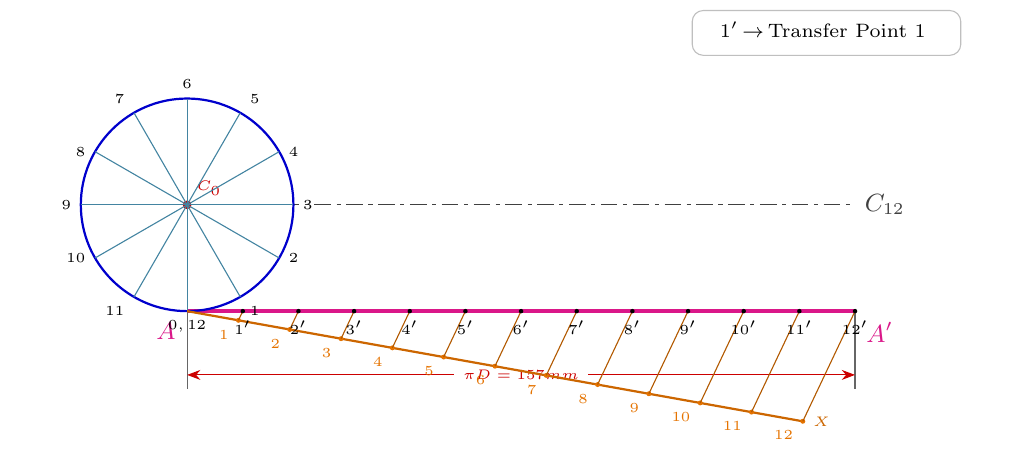
\begin{tikzpicture}[scale=0.45]
  \useasboundingbox (-4.5,-3.5) rectangle (22.5,8.0);
  \drawLegendCard{ \textbf{$1'$} & Transfer Point 1 }
  \draw[directrix line] (0,0) node[below left] {\small $A$} -- (18.85,0) node[below right] {\small $A'$};
  \draw[axis line] (0,3.0) -- (18.85,3.0) node[right] {\small $C_{12}$};
  \coordinate (C0) at (0,3.0);
  \fill[red!80!black] (C0) circle (3.5pt) node[above right, font=\tiny] {$C_0$};
  \draw[thick, blue!80!black] (C0) circle (3.0);
  \draw[thin, construction line] (0,0) -- (C0);
  \draw[thin, cyan!60!black, solid] (C0) -- (0,0);
  \draw[thin, cyan!60!black, solid] (C0) -- ++(300:3.0);
  \draw[thin, cyan!60!black, solid] (C0) -- ++(330:3.0);
  \draw[thin, cyan!60!black, solid] (C0) -- ++(0:3.0);
  \draw[thin, cyan!60!black, solid] (C0) -- ++(30:3.0);
  \draw[thin, cyan!60!black, solid] (C0) -- ++(60:3.0);
  \draw[thin, cyan!60!black, solid] (C0) -- ++(90:3.0);
  \draw[thin, cyan!60!black, solid] (C0) -- ++(120:3.0);
  \draw[thin, cyan!60!black, solid] (C0) -- ++(150:3.0);
  \draw[thin, cyan!60!black, solid] (C0) -- ++(180:3.0);
  \draw[thin, cyan!60!black, solid] (C0) -- ++(210:3.0);
  \draw[thin, cyan!60!black, solid] (C0) -- ++(240:3.0);
  \node[below, font=\tiny] at (0,0) {$0, 12$};
  \node[below right, font=\tiny] at (1.5,0.40) {1};
  \node[right, font=\tiny] at (2.598,1.5) {2};
  \node[right, font=\tiny] at (3.0,3.0) {3};
  \node[right, font=\tiny] at (2.598,4.5) {4};
  \node[above right, font=\tiny] at (1.5,5.598) {5};
  \node[above, font=\tiny] at (0,6.0) {6};
  \node[above left, font=\tiny] at (-1.5,5.598) {7};
  \node[left, font=\tiny] at (-2.598,4.5) {8};
  \node[left, font=\tiny] at (-3.0,3.0) {9};
  \node[left, font=\tiny] at (-2.598,1.5) {10};
  \node[below left, font=\tiny] at (-1.5,0.40) {11};
  \draw[dimension extension] (0,0) -- (0,-2.2);
  \draw[dimension extension] (18.85,0) -- (18.85,-2.2);
  \draw[<->, red!80!black, thin] (0,-1.8) -- (18.85,-1.8) node[midway, fill=white] {\tiny $\pi D = 157\text{ mm}$};
  \draw[thick, orange!80!black] (0,0) -- (17.38,-3.11) node[right, font=\tiny] {$X$};
  \foreach \i in {1,2,...,12} {
    \coordinate (a\i) at ({\i*1.448}, {-\i*0.259});
    \fill[orange!90!black] (a\i) circle (2.0pt);
    \node[below left, font=\tiny, orange!90!black] at (a\i) {\i};
  }
  \coordinate (a12) at ({12*1.448}, {-12*0.259});
  \draw[thin, orange!70!black, solid] (a12) -- (18.85, 0);
  \fill[black] (18.85, 0) circle (1.8pt);
  \node[below, font=\tiny] at (18.85, 0) {$12'$};
  \coordinate (a11) at ({11*1.448}, {-11*0.259});
  \draw[thin, orange!70!black, solid] (a11) -- ({11*1.5708}, 0);
  \fill[black] ({11*1.5708}, 0) circle (1.8pt);
  \node[below, font=\tiny] at ({11*1.5708}, 0) {$11'$};
  \coordinate (a10) at ({10*1.448}, {-10*0.259});
  \draw[thin, orange!70!black, solid] (a10) -- ({10*1.5708}, 0);
  \fill[black] ({10*1.5708}, 0) circle (1.8pt);
  \node[below, font=\tiny] at ({10*1.5708}, 0) {$10'$};
  \coordinate (a9) at ({9*1.448}, {-9*0.259});
  \draw[thin, orange!70!black, solid] (a9) -- ({9*1.5708}, 0);
  \fill[black] ({9*1.5708}, 0) circle (1.8pt);
  \node[below, font=\tiny] at ({9*1.5708}, 0) {$9'$};
  \coordinate (a8) at ({8*1.448}, {-8*0.259});
  \draw[thin, orange!70!black, solid] (a8) -- ({8*1.5708}, 0);
  \fill[black] ({8*1.5708}, 0) circle (1.8pt);
  \node[below, font=\tiny] at ({8*1.5708}, 0) {$8'$};
  \coordinate (a7) at ({7*1.448}, {-7*0.259});
  \draw[thin, orange!70!black, solid] (a7) -- ({7*1.5708}, 0);
  \fill[black] ({7*1.5708}, 0) circle (1.8pt);
  \node[below, font=\tiny] at ({7*1.5708}, 0) {$7'$};
  \coordinate (a6) at ({6*1.448}, {-6*0.259});
  \draw[thin, orange!70!black, solid] (a6) -- ({6*1.5708}, 0);
  \fill[black] ({6*1.5708}, 0) circle (1.8pt);
  \node[below, font=\tiny] at ({6*1.5708}, 0) {$6'$};
  \coordinate (a5) at ({5*1.448}, {-5*0.259});
  \draw[thin, orange!70!black, solid] (a5) -- ({5*1.5708}, 0);
  \fill[black] ({5*1.5708}, 0) circle (1.8pt);
  \node[below, font=\tiny] at ({5*1.5708}, 0) {$5'$};
  \coordinate (a4) at ({4*1.448}, {-4*0.259});
  \draw[thin, orange!70!black, solid] (a4) -- ({4*1.5708}, 0);
  \fill[black] ({4*1.5708}, 0) circle (1.8pt);
  \node[below, font=\tiny] at ({4*1.5708}, 0) {$4'$};
  \coordinate (a3) at ({3*1.448}, {-3*0.259});
  \draw[thin, orange!70!black, solid] (a3) -- ({3*1.5708}, 0);
  \fill[black] ({3*1.5708}, 0) circle (1.8pt);
  \node[below, font=\tiny] at ({3*1.5708}, 0) {$3'$};
  \coordinate (a2) at ({2*1.448}, {-2*0.259});
  \draw[thin, orange!70!black, solid] (a2) -- ({2*1.5708}, 0);
  \fill[black] ({2*1.5708}, 0) circle (1.8pt);
  \node[below, font=\tiny] at ({2*1.5708}, 0) {$2'$};
  \coordinate (a1) at ({1*1.448}, {-1*0.259});
  \draw[thin, orange!70!black, solid] (a1) -- ({1*1.5708}, 0);
  \fill[black] ({1*1.5708}, 0) circle (1.8pt);
  \node[below, font=\tiny] at ({1*1.5708}, 0) {$1'$};
\end{tikzpicture}
\end{frame}

% ============================================================
% STEP 4
% ============================================================
\renewcommand{\stepnum}{4}

\begin{frame}{Step 4: Project Divisions to Locate Centers $C_1\dots C_{12}$ (Base)}
\centering
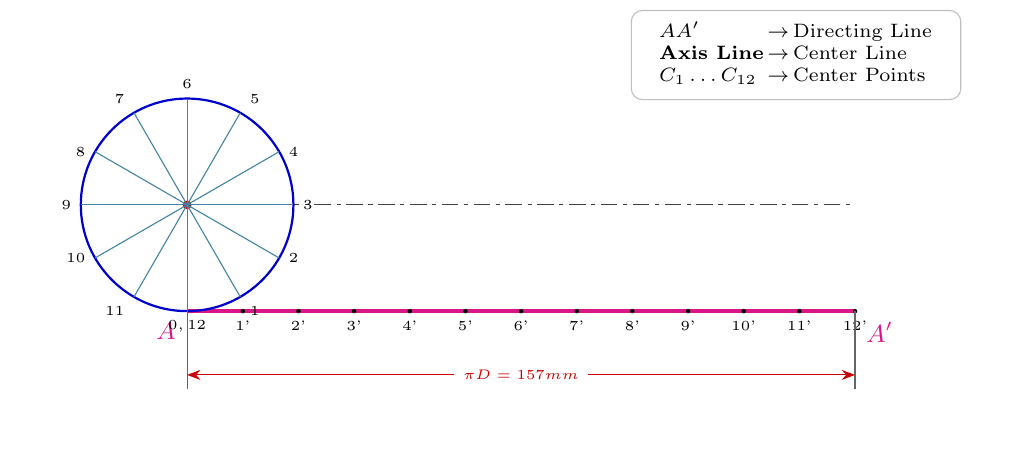
\begin{tikzpicture}[scale=0.45]
  \useasboundingbox (-4.5,-3.5) rectangle (22.5,8.0);
  \drawLegendCard{ \textbf{$AA'$} & Directing Line \\ \textbf{Axis Line} & Center Line \\ \textbf{$C_1\dots C_{12}$} & Center Points }
  \draw[directrix line] (0,0) node[below left] {\small $A$} -- (18.85,0) node[below right] {\small $A'$};
  \draw[axis line] (0,3.0) -- (18.85,3.0);
  \coordinate (C0) at (0,3.0);
  \fill[red!80!black] (C0) circle (3.5pt);
  \draw[thick, blue!80!black] (C0) circle (3.0);
  \draw[thin, construction line] (0,0) -- (C0);
  \draw[thin, cyan!60!black, solid] (C0) -- (0,0);
  \draw[thin, cyan!60!black, solid] (C0) -- ++(300:3.0);
  \draw[thin, cyan!60!black, solid] (C0) -- ++(330:3.0);
  \draw[thin, cyan!60!black, solid] (C0) -- ++(0:3.0);
  \draw[thin, cyan!60!black, solid] (C0) -- ++(30:3.0);
  \draw[thin, cyan!60!black, solid] (C0) -- ++(60:3.0);
  \draw[thin, cyan!60!black, solid] (C0) -- ++(90:3.0);
  \draw[thin, cyan!60!black, solid] (C0) -- ++(120:3.0);
  \draw[thin, cyan!60!black, solid] (C0) -- ++(150:3.0);
  \draw[thin, cyan!60!black, solid] (C0) -- ++(180:3.0);
  \draw[thin, cyan!60!black, solid] (C0) -- ++(210:3.0);
  \draw[thin, cyan!60!black, solid] (C0) -- ++(240:3.0);
  \node[below, font=\tiny] at (0,0) {$0, 12$};
  \node[below right, font=\tiny] at (1.5,0.40) {1};
  \node[right, font=\tiny] at (2.598,1.5) {2};
  \node[right, font=\tiny] at (3.0,3.0) {3};
  \node[right, font=\tiny] at (2.598,4.5) {4};
  \node[above right, font=\tiny] at (1.5,5.598) {5};
  \node[above, font=\tiny] at (0,6.0) {6};
  \node[above left, font=\tiny] at (-1.5,5.598) {7};
  \node[left, font=\tiny] at (-2.598,4.5) {8};
  \node[left, font=\tiny] at (-3.0,3.0) {9};
  \node[left, font=\tiny] at (-2.598,1.5) {10};
  \node[below left, font=\tiny] at (-1.5,0.40) {11};
  \foreach \i in {1,2,...,12} {
    \fill[black] ({\i*1.5708}, 0) circle (1.8pt);
    \node[below, font=\tiny] at ({\i*1.5708}, 0) {\i'};
  }
  \draw[dimension extension] (0,0) -- (0,-2.2);
  \draw[dimension extension] (18.85,0) -- (18.85,-2.2);
  \draw[<->, red!80!black, thin] (0,-1.8) -- (18.85,-1.8) node[midway, fill=white] {\tiny $\pi D = 157\text{ mm}$};
\end{tikzpicture}
\end{frame}

\foreach \n in {1,2,3,4,5,6,7,8,9,10,11,12} {
  \begin{frame}{Step 4: Project Divisions to Locate Centers $C_1\dots C_{12}$}
  \centering
  \begin{tikzpicture}[scale=0.45]
    \useasboundingbox (-4.5,-3.5) rectangle (22.5,8.0);
    \drawLegendCard{ \textbf{$AA'$} & Directing Line \\ \textbf{Axis Line} & Center Line \\ \textbf{$C_1\dots C_{12}$} & Center Points }
    \draw[directrix line] (0,0) node[below left] {\small $A$} -- (18.85,0) node[below right] {\small $A'$};
    \draw[axis line] (0,3.0) -- (18.85,3.0);
    \coordinate (C0) at (0,3.0);
    \fill[red!80!black] (C0) circle (3.5pt);
    \draw[thick, blue!80!black] (C0) circle (3.0);
    \draw[thin, construction line] (0,0) -- (C0);
    \draw[thin, cyan!60!black, solid] (C0) -- (0,0);
    \draw[thin, cyan!60!black, solid] (C0) -- ++(300:3.0);
    \draw[thin, cyan!60!black, solid] (C0) -- ++(330:3.0);
    \draw[thin, cyan!60!black, solid] (C0) -- ++(0:3.0);
    \draw[thin, cyan!60!black, solid] (C0) -- ++(30:3.0);
    \draw[thin, cyan!60!black, solid] (C0) -- ++(60:3.0);
    \draw[thin, cyan!60!black, solid] (C0) -- ++(90:3.0);
    \draw[thin, cyan!60!black, solid] (C0) -- ++(120:3.0);
    \draw[thin, cyan!60!black, solid] (C0) -- ++(150:3.0);
    \draw[thin, cyan!60!black, solid] (C0) -- ++(180:3.0);
    \draw[thin, cyan!60!black, solid] (C0) -- ++(210:3.0);
    \draw[thin, cyan!60!black, solid] (C0) -- ++(240:3.0);
    \node[below, font=\tiny] at (0,0) {$0, 12$};
    \node[below right, font=\tiny] at (1.5,0.40) {1};
    \node[right, font=\tiny] at (2.598,1.5) {2};
    \node[right, font=\tiny] at (3.0,3.0) {3};
    \node[right, font=\tiny] at (2.598,4.5) {4};
    \node[above right, font=\tiny] at (1.5,5.598) {5};
    \node[above, font=\tiny] at (0,6.0) {6};
    \node[above left, font=\tiny] at (-1.5,5.598) {7};
    \node[left, font=\tiny] at (-2.598,4.5) {8};
    \node[left, font=\tiny] at (-3.0,3.0) {9};
    \node[left, font=\tiny] at (-2.598,1.5) {10};
    \node[below left, font=\tiny] at (-1.5,0.40) {11};
    \foreach \i in {1,2,...,12} {
      \fill[black] ({\i*1.5708}, 0) circle (1.8pt);
      \node[below, font=\tiny] at ({\i*1.5708}, 0) {\i'};
    }
    \draw[dimension extension] (0,0) -- (0,-2.2);
    \draw[dimension extension] (18.85,0) -- (18.85,-2.2);
    \draw[<->, red!80!black, thin] (0,-1.8) -- (18.85,-1.8) node[midway, fill=white] {\tiny $\pi D = 157\text{ mm}$};
    \foreach \i in {1,...,\n} {
      \coordinate (C\i) at ({\i*1.5708}, 3.0);
      \draw[thin, black!40, solid] ({\i*1.5708}, 0) -- (C\i);
      \fill[red!80!black] (C\i) circle (2.5pt);
      \node[above=1pt, font=\tiny, red!80!black] at (C\i) {$C_{\i}$};
    }
  \end{tikzpicture}
  \end{frame}
}

% ============================================================
% STEP 5
% ============================================================
\renewcommand{\stepnum}{5}

\begin{frame}{Step 5: Draw Horizontal Reference Lines (Base)}
\centering
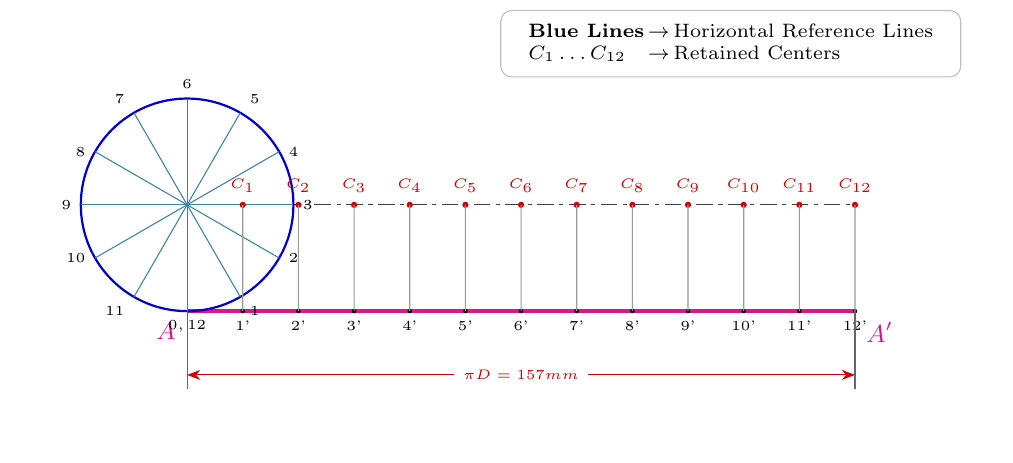
\begin{tikzpicture}[scale=0.45]
  \useasboundingbox (-4.5,-3.5) rectangle (22.5,8.0);
  \drawLegendCard{ \textbf{Blue Lines} & Horizontal Reference Lines \\ \textbf{$C_1\dots C_{12}$} & Retained Centers }
  \draw[directrix line] (0,0) node[below left] {\small $A$} -- (18.85,0) node[below right] {\small $A'$};
  \draw[axis line] (0,3.0) -- (18.85,3.0);
  \coordinate (C0) at (0,3.0); \draw[thick, blue!80!black] (C0) circle (3.0);
  \draw[thin, construction line] (0,0) -- (C0);
  \draw[thin, cyan!60!black, solid] (C0) -- (0,0);
  \draw[thin, cyan!60!black, solid] (C0) -- ++(300:3.0);
  \draw[thin, cyan!60!black, solid] (C0) -- ++(330:3.0);
  \draw[thin, cyan!60!black, solid] (C0) -- ++(0:3.0);
  \draw[thin, cyan!60!black, solid] (C0) -- ++(30:3.0);
  \draw[thin, cyan!60!black, solid] (C0) -- ++(60:3.0);
  \draw[thin, cyan!60!black, solid] (C0) -- ++(90:3.0);
  \draw[thin, cyan!60!black, solid] (C0) -- ++(120:3.0);
  \draw[thin, cyan!60!black, solid] (C0) -- ++(150:3.0);
  \draw[thin, cyan!60!black, solid] (C0) -- ++(180:3.0);
  \draw[thin, cyan!60!black, solid] (C0) -- ++(210:3.0);
  \draw[thin, cyan!60!black, solid] (C0) -- ++(240:3.0);
  \node[below, font=\tiny] at (0,0) {$0, 12$};
  \node[below right, font=\tiny] at (1.5,0.40) {1};
  \node[right, font=\tiny] at (2.598,1.5) {2};
  \node[right, font=\tiny] at (3.0,3.0) {3};
  \node[right, font=\tiny] at (2.598,4.5) {4};
  \node[above right, font=\tiny] at (1.5,5.598) {5};
  \node[above, font=\tiny] at (0,6.0) {6};
  \node[above left, font=\tiny] at (-1.5,5.598) {7};
  \node[left, font=\tiny] at (-2.598,4.5) {8};
  \node[left, font=\tiny] at (-3.0,3.0) {9};
  \node[left, font=\tiny] at (-2.598,1.5) {10};
  \node[below left, font=\tiny] at (-1.5,0.40) {11};
  \foreach \i in {1,2,...,12} { 
    \fill[black] ({\i*1.5708}, 0) circle (1.8pt);
    \node[below, font=\tiny] at ({\i*1.5708}, 0) {\i'};
    \fill[red!80!black] ({\i*1.5708}, 3.0) circle (2.5pt);
    \node[above=1pt, font=\tiny, red!80!black] at ({\i*1.5708}, 3.0) {$C_{\i}$};
    \coordinate (C\i) at ({\i*1.5708}, 3.0);
    \draw[thin, black!40, solid] ({\i*1.5708}, 0) -- (C\i);
  }
  \draw[dimension extension] (0,0) -- (0,-2.2);
  \draw[dimension extension] (18.85,0) -- (18.85,-2.2);
  \draw[<->, red!80!black, thin] (0,-1.8) -- (18.85,-1.8) node[midway, fill=white] {\tiny $\pi D = 157\text{ mm}$};
\end{tikzpicture}
\end{frame}

\begin{frame}{Step 5: Draw Horizontal Reference Lines}
\centering
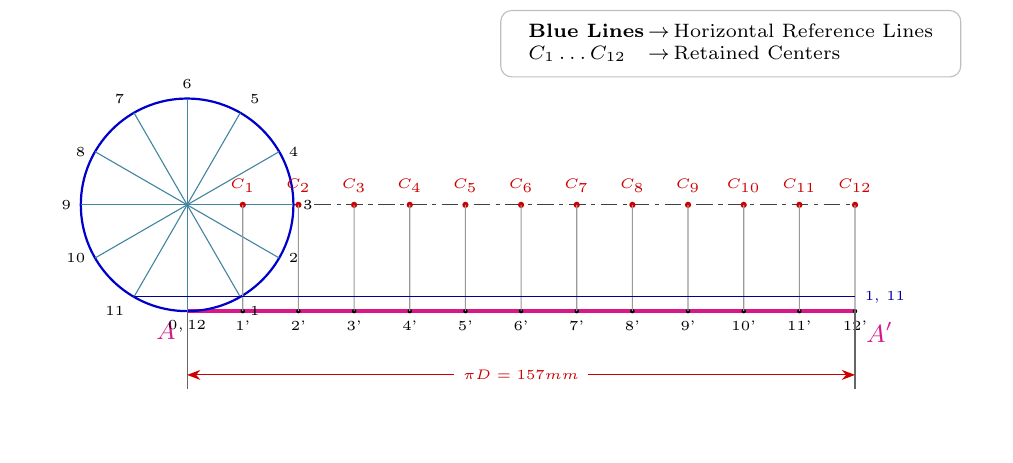
\begin{tikzpicture}[scale=0.45]
  \useasboundingbox (-4.5,-3.5) rectangle (22.5,8.0);
  \drawLegendCard{ \textbf{Blue Lines} & Horizontal Reference Lines \\ \textbf{$C_1\dots C_{12}$} & Retained Centers }
  \draw[directrix line] (0,0) node[below left] {\small $A$} -- (18.85,0) node[below right] {\small $A'$};
  \draw[axis line] (0,3.0) -- (18.85,3.0);
  \coordinate (C0) at (0,3.0); \draw[thick, blue!80!black] (C0) circle (3.0);
  \draw[thin, construction line] (0,0) -- (C0);
  \draw[thin, cyan!60!black, solid] (C0) -- (0,0);
  \draw[thin, cyan!60!black, solid] (C0) -- ++(300:3.0);
  \draw[thin, cyan!60!black, solid] (C0) -- ++(330:3.0);
  \draw[thin, cyan!60!black, solid] (C0) -- ++(0:3.0);
  \draw[thin, cyan!60!black, solid] (C0) -- ++(30:3.0);
  \draw[thin, cyan!60!black, solid] (C0) -- ++(60:3.0);
  \draw[thin, cyan!60!black, solid] (C0) -- ++(90:3.0);
  \draw[thin, cyan!60!black, solid] (C0) -- ++(120:3.0);
  \draw[thin, cyan!60!black, solid] (C0) -- ++(150:3.0);
  \draw[thin, cyan!60!black, solid] (C0) -- ++(180:3.0);
  \draw[thin, cyan!60!black, solid] (C0) -- ++(210:3.0);
  \draw[thin, cyan!60!black, solid] (C0) -- ++(240:3.0);
  \node[below, font=\tiny] at (0,0) {$0, 12$};
  \node[below right, font=\tiny] at (1.5,0.40) {1};
  \node[right, font=\tiny] at (2.598,1.5) {2};
  \node[right, font=\tiny] at (3.0,3.0) {3};
  \node[right, font=\tiny] at (2.598,4.5) {4};
  \node[above right, font=\tiny] at (1.5,5.598) {5};
  \node[above, font=\tiny] at (0,6.0) {6};
  \node[above left, font=\tiny] at (-1.5,5.598) {7};
  \node[left, font=\tiny] at (-2.598,4.5) {8};
  \node[left, font=\tiny] at (-3.0,3.0) {9};
  \node[left, font=\tiny] at (-2.598,1.5) {10};
  \node[below left, font=\tiny] at (-1.5,0.40) {11};
  \foreach \i in {1,2,...,12} { 
    \fill[black] ({\i*1.5708}, 0) circle (1.8pt);
    \node[below, font=\tiny] at ({\i*1.5708}, 0) {\i'};
    \fill[red!80!black] ({\i*1.5708}, 3.0) circle (2.5pt);
    \node[above=1pt, font=\tiny, red!80!black] at ({\i*1.5708}, 3.0) {$C_{\i}$};
    \coordinate (C\i) at ({\i*1.5708}, 3.0);
    \draw[thin, black!40, solid] ({\i*1.5708}, 0) -- (C\i);
  }
  \draw[dimension extension] (0,0) -- (0,-2.2);
  \draw[dimension extension] (18.85,0) -- (18.85,-2.2);
  \draw[<->, red!80!black, thin] (0,-1.8) -- (18.85,-1.8) node[midway, fill=white] {\tiny $\pi D = 157\text{ mm}$};
  \draw[construction line] (-1.500, 0.402) -- (18.85, 0.402) node[right, font=\tiny] {1, 11};
\end{tikzpicture}
\end{frame}

\begin{frame}{Step 5: Draw Horizontal Reference Lines}
\centering
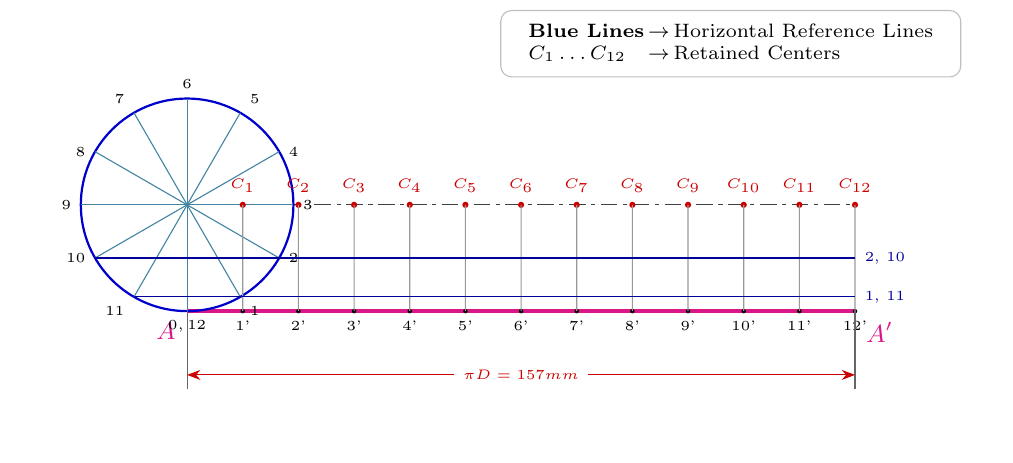
\begin{tikzpicture}[scale=0.45]
  \useasboundingbox (-4.5,-3.5) rectangle (22.5,8.0);
  \drawLegendCard{ \textbf{Blue Lines} & Horizontal Reference Lines \\ \textbf{$C_1\dots C_{12}$} & Retained Centers }
  \draw[directrix line] (0,0) node[below left] {\small $A$} -- (18.85,0) node[below right] {\small $A'$};
  \draw[axis line] (0,3.0) -- (18.85,3.0);
  \coordinate (C0) at (0,3.0); \draw[thick, blue!80!black] (C0) circle (3.0);
  \draw[thin, construction line] (0,0) -- (C0);
  \draw[thin, cyan!60!black, solid] (C0) -- (0,0);
  \draw[thin, cyan!60!black, solid] (C0) -- ++(300:3.0);
  \draw[thin, cyan!60!black, solid] (C0) -- ++(330:3.0);
  \draw[thin, cyan!60!black, solid] (C0) -- ++(0:3.0);
  \draw[thin, cyan!60!black, solid] (C0) -- ++(30:3.0);
  \draw[thin, cyan!60!black, solid] (C0) -- ++(60:3.0);
  \draw[thin, cyan!60!black, solid] (C0) -- ++(90:3.0);
  \draw[thin, cyan!60!black, solid] (C0) -- ++(120:3.0);
  \draw[thin, cyan!60!black, solid] (C0) -- ++(150:3.0);
  \draw[thin, cyan!60!black, solid] (C0) -- ++(180:3.0);
  \draw[thin, cyan!60!black, solid] (C0) -- ++(210:3.0);
  \draw[thin, cyan!60!black, solid] (C0) -- ++(240:3.0);
  \node[below, font=\tiny] at (0,0) {$0, 12$};
  \node[below right, font=\tiny] at (1.5,0.40) {1};
  \node[right, font=\tiny] at (2.598,1.5) {2};
  \node[right, font=\tiny] at (3.0,3.0) {3};
  \node[right, font=\tiny] at (2.598,4.5) {4};
  \node[above right, font=\tiny] at (1.5,5.598) {5};
  \node[above, font=\tiny] at (0,6.0) {6};
  \node[above left, font=\tiny] at (-1.5,5.598) {7};
  \node[left, font=\tiny] at (-2.598,4.5) {8};
  \node[left, font=\tiny] at (-3.0,3.0) {9};
  \node[left, font=\tiny] at (-2.598,1.5) {10};
  \node[below left, font=\tiny] at (-1.5,0.40) {11};
  \foreach \i in {1,2,...,12} { 
    \fill[black] ({\i*1.5708}, 0) circle (1.8pt);
    \node[below, font=\tiny] at ({\i*1.5708}, 0) {\i'};
    \fill[red!80!black] ({\i*1.5708}, 3.0) circle (2.5pt);
    \node[above=1pt, font=\tiny, red!80!black] at ({\i*1.5708}, 3.0) {$C_{\i}$};
    \coordinate (C\i) at ({\i*1.5708}, 3.0);
    \draw[thin, black!40, solid] ({\i*1.5708}, 0) -- (C\i);
  }
  \draw[dimension extension] (0,0) -- (0,-2.2);
  \draw[dimension extension] (18.85,0) -- (18.85,-2.2);
  \draw[<->, red!80!black, thin] (0,-1.8) -- (18.85,-1.8) node[midway, fill=white] {\tiny $\pi D = 157\text{ mm}$};
  \draw[construction line] (-1.500, 0.402) -- (18.85, 0.402) node[right, font=\tiny] {1, 11};
  \draw[construction line] (-2.598, 1.500) -- (18.85, 1.500) node[right, font=\tiny] {2, 10};
\end{tikzpicture}
\end{frame}

\begin{frame}{Step 5: Draw Horizontal Reference Lines}
\centering
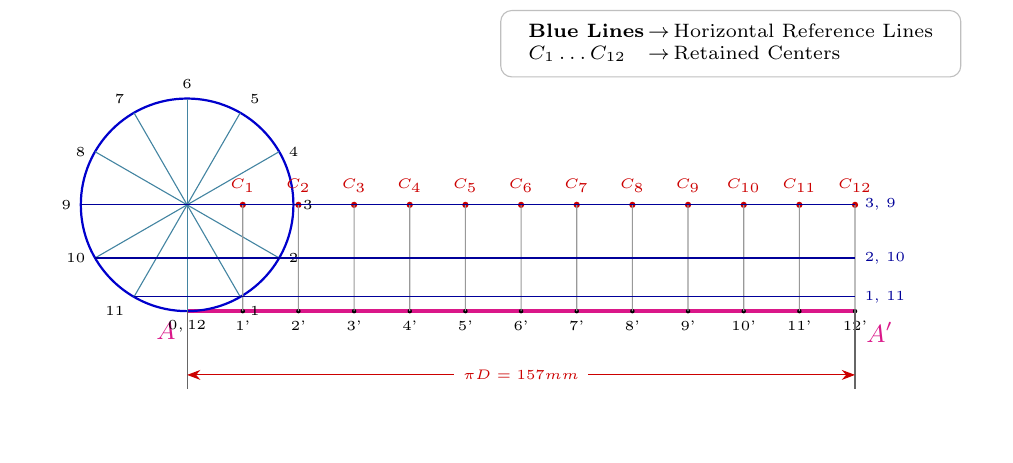
\begin{tikzpicture}[scale=0.45]
  \useasboundingbox (-4.5,-3.5) rectangle (22.5,8.0);
  \drawLegendCard{ \textbf{Blue Lines} & Horizontal Reference Lines \\ \textbf{$C_1\dots C_{12}$} & Retained Centers }
  \draw[directrix line] (0,0) node[below left] {\small $A$} -- (18.85,0) node[below right] {\small $A'$};
  \draw[axis line] (0,3.0) -- (18.85,3.0);
  \coordinate (C0) at (0,3.0); \draw[thick, blue!80!black] (C0) circle (3.0);
  \draw[thin, construction line] (0,0) -- (C0);
  \draw[thin, cyan!60!black, solid] (C0) -- (0,0);
  \draw[thin, cyan!60!black, solid] (C0) -- ++(300:3.0);
  \draw[thin, cyan!60!black, solid] (C0) -- ++(330:3.0);
  \draw[thin, cyan!60!black, solid] (C0) -- ++(0:3.0);
  \draw[thin, cyan!60!black, solid] (C0) -- ++(30:3.0);
  \draw[thin, cyan!60!black, solid] (C0) -- ++(60:3.0);
  \draw[thin, cyan!60!black, solid] (C0) -- ++(90:3.0);
  \draw[thin, cyan!60!black, solid] (C0) -- ++(120:3.0);
  \draw[thin, cyan!60!black, solid] (C0) -- ++(150:3.0);
  \draw[thin, cyan!60!black, solid] (C0) -- ++(180:3.0);
  \draw[thin, cyan!60!black, solid] (C0) -- ++(210:3.0);
  \draw[thin, cyan!60!black, solid] (C0) -- ++(240:3.0);
  \node[below, font=\tiny] at (0,0) {$0, 12$};
  \node[below right, font=\tiny] at (1.5,0.40) {1};
  \node[right, font=\tiny] at (2.598,1.5) {2};
  \node[right, font=\tiny] at (3.0,3.0) {3};
  \node[right, font=\tiny] at (2.598,4.5) {4};
  \node[above right, font=\tiny] at (1.5,5.598) {5};
  \node[above, font=\tiny] at (0,6.0) {6};
  \node[above left, font=\tiny] at (-1.5,5.598) {7};
  \node[left, font=\tiny] at (-2.598,4.5) {8};
  \node[left, font=\tiny] at (-3.0,3.0) {9};
  \node[left, font=\tiny] at (-2.598,1.5) {10};
  \node[below left, font=\tiny] at (-1.5,0.40) {11};
  \foreach \i in {1,2,...,12} { 
    \fill[black] ({\i*1.5708}, 0) circle (1.8pt);
    \node[below, font=\tiny] at ({\i*1.5708}, 0) {\i'};
    \fill[red!80!black] ({\i*1.5708}, 3.0) circle (2.5pt);
    \node[above=1pt, font=\tiny, red!80!black] at ({\i*1.5708}, 3.0) {$C_{\i}$};
    \coordinate (C\i) at ({\i*1.5708}, 3.0);
    \draw[thin, black!40, solid] ({\i*1.5708}, 0) -- (C\i);
  }
  \draw[dimension extension] (0,0) -- (0,-2.2);
  \draw[dimension extension] (18.85,0) -- (18.85,-2.2);
  \draw[<->, red!80!black, thin] (0,-1.8) -- (18.85,-1.8) node[midway, fill=white] {\tiny $\pi D = 157\text{ mm}$};
  \draw[construction line] (-1.500, 0.402) -- (18.85, 0.402) node[right, font=\tiny] {1, 11};
  \draw[construction line] (-2.598, 1.500) -- (18.85, 1.500) node[right, font=\tiny] {2, 10};
  \draw[construction line] (-3.000, 3.000) -- (18.85, 3.000) node[right, font=\tiny] {3, 9};
\end{tikzpicture}
\end{frame}

\begin{frame}{Step 5: Draw Horizontal Reference Lines}
\centering
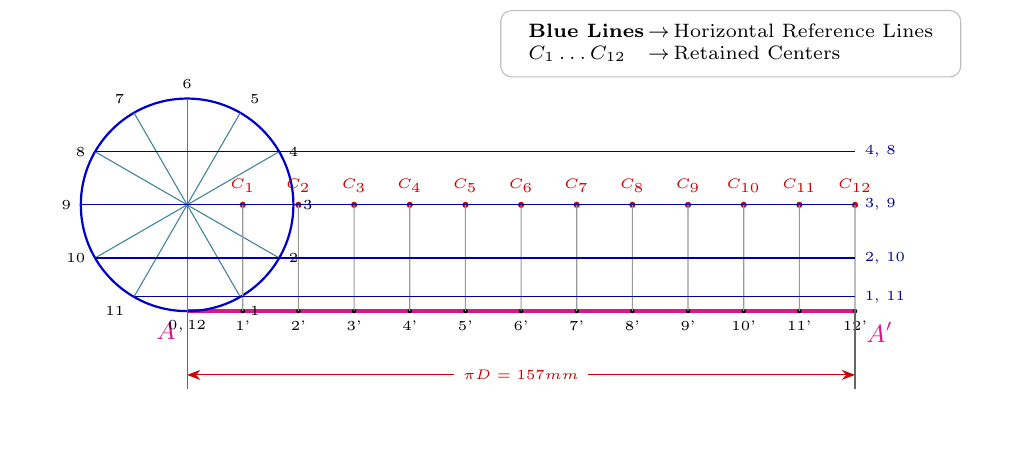
\begin{tikzpicture}[scale=0.45]
  \useasboundingbox (-4.5,-3.5) rectangle (22.5,8.0);
  \drawLegendCard{ \textbf{Blue Lines} & Horizontal Reference Lines \\ \textbf{$C_1\dots C_{12}$} & Retained Centers }
  \draw[directrix line] (0,0) node[below left] {\small $A$} -- (18.85,0) node[below right] {\small $A'$};
  \draw[axis line] (0,3.0) -- (18.85,3.0);
  \coordinate (C0) at (0,3.0); \draw[thick, blue!80!black] (C0) circle (3.0);
  \draw[thin, construction line] (0,0) -- (C0);
  \draw[thin, cyan!60!black, solid] (C0) -- (0,0);
  \draw[thin, cyan!60!black, solid] (C0) -- ++(300:3.0);
  \draw[thin, cyan!60!black, solid] (C0) -- ++(330:3.0);
  \draw[thin, cyan!60!black, solid] (C0) -- ++(0:3.0);
  \draw[thin, cyan!60!black, solid] (C0) -- ++(30:3.0);
  \draw[thin, cyan!60!black, solid] (C0) -- ++(60:3.0);
  \draw[thin, cyan!60!black, solid] (C0) -- ++(90:3.0);
  \draw[thin, cyan!60!black, solid] (C0) -- ++(120:3.0);
  \draw[thin, cyan!60!black, solid] (C0) -- ++(150:3.0);
  \draw[thin, cyan!60!black, solid] (C0) -- ++(180:3.0);
  \draw[thin, cyan!60!black, solid] (C0) -- ++(210:3.0);
  \draw[thin, cyan!60!black, solid] (C0) -- ++(240:3.0);
  \node[below, font=\tiny] at (0,0) {$0, 12$};
  \node[below right, font=\tiny] at (1.5,0.40) {1};
  \node[right, font=\tiny] at (2.598,1.5) {2};
  \node[right, font=\tiny] at (3.0,3.0) {3};
  \node[right, font=\tiny] at (2.598,4.5) {4};
  \node[above right, font=\tiny] at (1.5,5.598) {5};
  \node[above, font=\tiny] at (0,6.0) {6};
  \node[above left, font=\tiny] at (-1.5,5.598) {7};
  \node[left, font=\tiny] at (-2.598,4.5) {8};
  \node[left, font=\tiny] at (-3.0,3.0) {9};
  \node[left, font=\tiny] at (-2.598,1.5) {10};
  \node[below left, font=\tiny] at (-1.5,0.40) {11};
  \foreach \i in {1,2,...,12} { 
    \fill[black] ({\i*1.5708}, 0) circle (1.8pt);
    \node[below, font=\tiny] at ({\i*1.5708}, 0) {\i'};
    \fill[red!80!black] ({\i*1.5708}, 3.0) circle (2.5pt);
    \node[above=1pt, font=\tiny, red!80!black] at ({\i*1.5708}, 3.0) {$C_{\i}$};
    \coordinate (C\i) at ({\i*1.5708}, 3.0);
    \draw[thin, black!40, solid] ({\i*1.5708}, 0) -- (C\i);
  }
  \draw[dimension extension] (0,0) -- (0,-2.2);
  \draw[dimension extension] (18.85,0) -- (18.85,-2.2);
  \draw[<->, red!80!black, thin] (0,-1.8) -- (18.85,-1.8) node[midway, fill=white] {\tiny $\pi D = 157\text{ mm}$};
  \draw[construction line] (-1.500, 0.402) -- (18.85, 0.402) node[right, font=\tiny] {1, 11};
  \draw[construction line] (-2.598, 1.500) -- (18.85, 1.500) node[right, font=\tiny] {2, 10};
  \draw[construction line] (-3.000, 3.000) -- (18.85, 3.000) node[right, font=\tiny] {3, 9};
  \draw[construction line] (-2.598, 4.500) -- (18.85, 4.500) node[right, font=\tiny] {4, 8};
\end{tikzpicture}
\end{frame}

\begin{frame}{Step 5: Draw Horizontal Reference Lines}
\centering
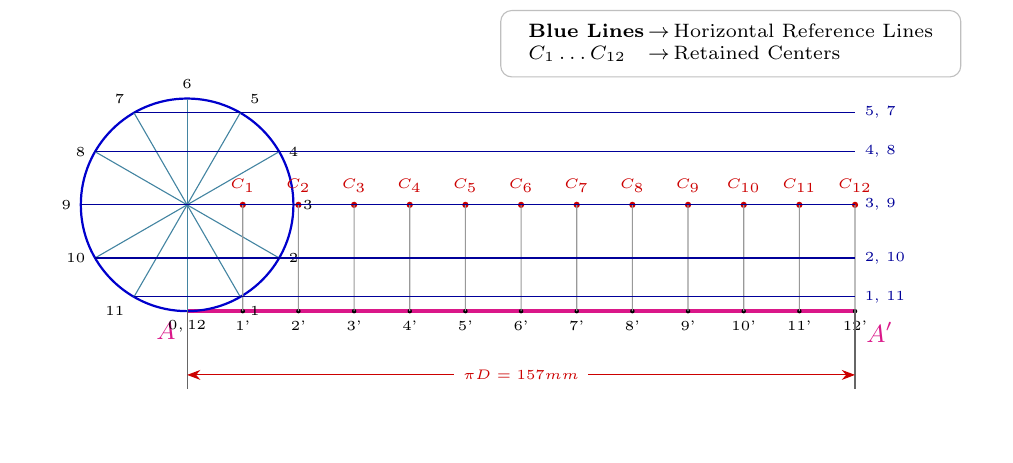
\begin{tikzpicture}[scale=0.45]
  \useasboundingbox (-4.5,-3.5) rectangle (22.5,8.0);
  \drawLegendCard{ \textbf{Blue Lines} & Horizontal Reference Lines \\ \textbf{$C_1\dots C_{12}$} & Retained Centers }
  \draw[directrix line] (0,0) node[below left] {\small $A$} -- (18.85,0) node[below right] {\small $A'$};
  \draw[axis line] (0,3.0) -- (18.85,3.0);
  \coordinate (C0) at (0,3.0); \draw[thick, blue!80!black] (C0) circle (3.0);
  \draw[thin, construction line] (0,0) -- (C0);
  \draw[thin, cyan!60!black, solid] (C0) -- (0,0);
  \draw[thin, cyan!60!black, solid] (C0) -- ++(300:3.0);
  \draw[thin, cyan!60!black, solid] (C0) -- ++(330:3.0);
  \draw[thin, cyan!60!black, solid] (C0) -- ++(0:3.0);
  \draw[thin, cyan!60!black, solid] (C0) -- ++(30:3.0);
  \draw[thin, cyan!60!black, solid] (C0) -- ++(60:3.0);
  \draw[thin, cyan!60!black, solid] (C0) -- ++(90:3.0);
  \draw[thin, cyan!60!black, solid] (C0) -- ++(120:3.0);
  \draw[thin, cyan!60!black, solid] (C0) -- ++(150:3.0);
  \draw[thin, cyan!60!black, solid] (C0) -- ++(180:3.0);
  \draw[thin, cyan!60!black, solid] (C0) -- ++(210:3.0);
  \draw[thin, cyan!60!black, solid] (C0) -- ++(240:3.0);
  \node[below, font=\tiny] at (0,0) {$0, 12$};
  \node[below right, font=\tiny] at (1.5,0.40) {1};
  \node[right, font=\tiny] at (2.598,1.5) {2};
  \node[right, font=\tiny] at (3.0,3.0) {3};
  \node[right, font=\tiny] at (2.598,4.5) {4};
  \node[above right, font=\tiny] at (1.5,5.598) {5};
  \node[above, font=\tiny] at (0,6.0) {6};
  \node[above left, font=\tiny] at (-1.5,5.598) {7};
  \node[left, font=\tiny] at (-2.598,4.5) {8};
  \node[left, font=\tiny] at (-3.0,3.0) {9};
  \node[left, font=\tiny] at (-2.598,1.5) {10};
  \node[below left, font=\tiny] at (-1.5,0.40) {11};
  \foreach \i in {1,2,...,12} { 
    \fill[black] ({\i*1.5708}, 0) circle (1.8pt);
    \node[below, font=\tiny] at ({\i*1.5708}, 0) {\i'};
    \fill[red!80!black] ({\i*1.5708}, 3.0) circle (2.5pt);
    \node[above=1pt, font=\tiny, red!80!black] at ({\i*1.5708}, 3.0) {$C_{\i}$};
    \coordinate (C\i) at ({\i*1.5708}, 3.0);
    \draw[thin, black!40, solid] ({\i*1.5708}, 0) -- (C\i);
  }
  \draw[dimension extension] (0,0) -- (0,-2.2);
  \draw[dimension extension] (18.85,0) -- (18.85,-2.2);
  \draw[<->, red!80!black, thin] (0,-1.8) -- (18.85,-1.8) node[midway, fill=white] {\tiny $\pi D = 157\text{ mm}$};
  \draw[construction line] (-1.500, 0.402) -- (18.85, 0.402) node[right, font=\tiny] {1, 11};
  \draw[construction line] (-2.598, 1.500) -- (18.85, 1.500) node[right, font=\tiny] {2, 10};
  \draw[construction line] (-3.000, 3.000) -- (18.85, 3.000) node[right, font=\tiny] {3, 9};
  \draw[construction line] (-2.598, 4.500) -- (18.85, 4.500) node[right, font=\tiny] {4, 8};
  \draw[construction line] (-1.500, 5.598) -- (18.85, 5.598) node[right, font=\tiny] {5, 7};
\end{tikzpicture}
\end{frame}

\begin{frame}{Step 5: Draw Horizontal Reference Lines}
\centering
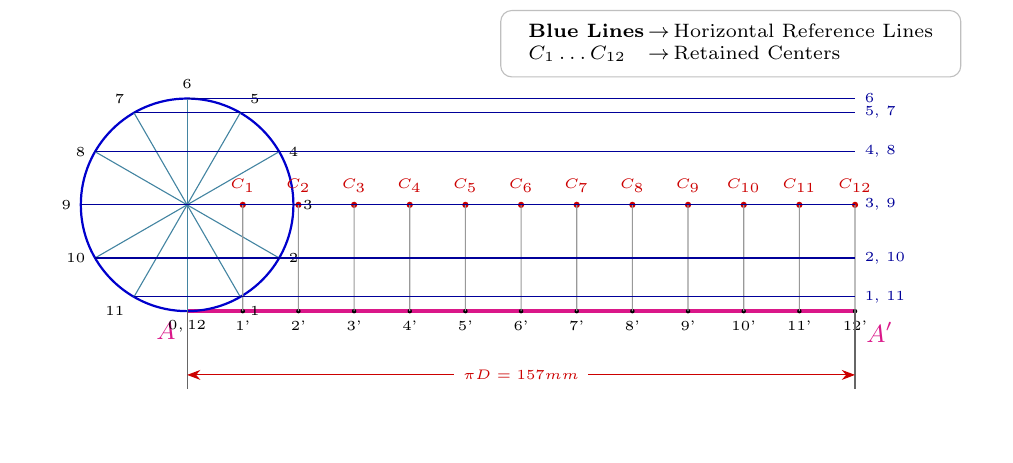
\begin{tikzpicture}[scale=0.45]
  \useasboundingbox (-4.5,-3.5) rectangle (22.5,8.0);
  \drawLegendCard{ \textbf{Blue Lines} & Horizontal Reference Lines \\ \textbf{$C_1\dots C_{12}$} & Retained Centers }
  \draw[directrix line] (0,0) node[below left] {\small $A$} -- (18.85,0) node[below right] {\small $A'$};
  \draw[axis line] (0,3.0) -- (18.85,3.0);
  \coordinate (C0) at (0,3.0); \draw[thick, blue!80!black] (C0) circle (3.0);
  \draw[thin, construction line] (0,0) -- (C0);
  \draw[thin, cyan!60!black, solid] (C0) -- (0,0);
  \draw[thin, cyan!60!black, solid] (C0) -- ++(300:3.0);
  \draw[thin, cyan!60!black, solid] (C0) -- ++(330:3.0);
  \draw[thin, cyan!60!black, solid] (C0) -- ++(0:3.0);
  \draw[thin, cyan!60!black, solid] (C0) -- ++(30:3.0);
  \draw[thin, cyan!60!black, solid] (C0) -- ++(60:3.0);
  \draw[thin, cyan!60!black, solid] (C0) -- ++(90:3.0);
  \draw[thin, cyan!60!black, solid] (C0) -- ++(120:3.0);
  \draw[thin, cyan!60!black, solid] (C0) -- ++(150:3.0);
  \draw[thin, cyan!60!black, solid] (C0) -- ++(180:3.0);
  \draw[thin, cyan!60!black, solid] (C0) -- ++(210:3.0);
  \draw[thin, cyan!60!black, solid] (C0) -- ++(240:3.0);
  \node[below, font=\tiny] at (0,0) {$0, 12$};
  \node[below right, font=\tiny] at (1.5,0.40) {1};
  \node[right, font=\tiny] at (2.598,1.5) {2};
  \node[right, font=\tiny] at (3.0,3.0) {3};
  \node[right, font=\tiny] at (2.598,4.5) {4};
  \node[above right, font=\tiny] at (1.5,5.598) {5};
  \node[above, font=\tiny] at (0,6.0) {6};
  \node[above left, font=\tiny] at (-1.5,5.598) {7};
  \node[left, font=\tiny] at (-2.598,4.5) {8};
  \node[left, font=\tiny] at (-3.0,3.0) {9};
  \node[left, font=\tiny] at (-2.598,1.5) {10};
  \node[below left, font=\tiny] at (-1.5,0.40) {11};
  \foreach \i in {1,2,...,12} { 
    \fill[black] ({\i*1.5708}, 0) circle (1.8pt);
    \node[below, font=\tiny] at ({\i*1.5708}, 0) {\i'};
    \fill[red!80!black] ({\i*1.5708}, 3.0) circle (2.5pt);
    \node[above=1pt, font=\tiny, red!80!black] at ({\i*1.5708}, 3.0) {$C_{\i}$};
    \coordinate (C\i) at ({\i*1.5708}, 3.0);
    \draw[thin, black!40, solid] ({\i*1.5708}, 0) -- (C\i);
  }
  \draw[dimension extension] (0,0) -- (0,-2.2);
  \draw[dimension extension] (18.85,0) -- (18.85,-2.2);
  \draw[<->, red!80!black, thin] (0,-1.8) -- (18.85,-1.8) node[midway, fill=white] {\tiny $\pi D = 157\text{ mm}$};
  \draw[construction line] (-1.500, 0.402) -- (18.85, 0.402) node[right, font=\tiny] {1, 11};
  \draw[construction line] (-2.598, 1.500) -- (18.85, 1.500) node[right, font=\tiny] {2, 10};
  \draw[construction line] (-3.000, 3.000) -- (18.85, 3.000) node[right, font=\tiny] {3, 9};
  \draw[construction line] (-2.598, 4.500) -- (18.85, 4.500) node[right, font=\tiny] {4, 8};
  \draw[construction line] (-1.500, 5.598) -- (18.85, 5.598) node[right, font=\tiny] {5, 7};
  \draw[construction line] (0.000, 6.000) -- (18.85, 6.000) node[right, font=\tiny] {6};
\end{tikzpicture}
\end{frame}

% ============================================================
% STEP 6
% ============================================================
\renewcommand{\stepnum}{6}

\begin{frame}{Step 6: Strike Cutting Arcs (Radius = 25 mm) to Locate $P_0$}
\centering
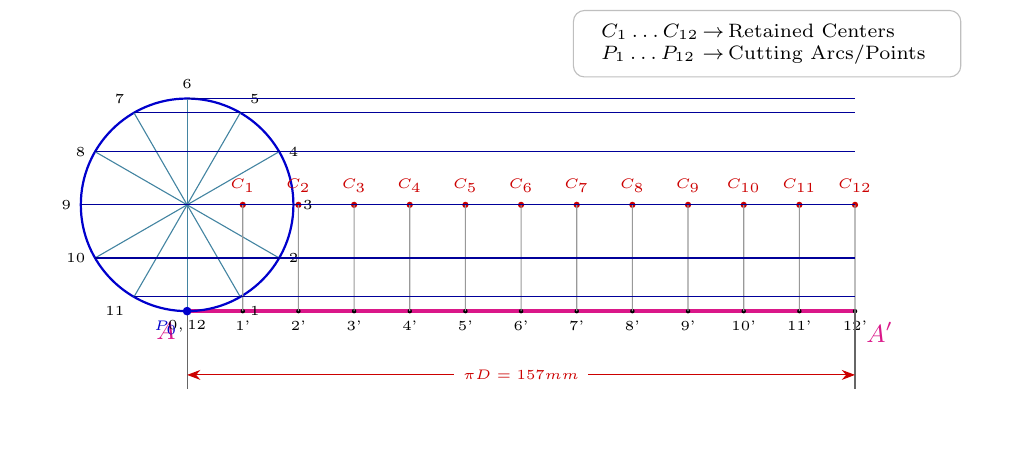
\begin{tikzpicture}[scale=0.45]
  \useasboundingbox (-4.5,-3.5) rectangle (22.5,8.0);
  \drawLegendCard{ \textbf{$C_1\dots C_{12}$} & Retained Centers \\ \textbf{$P_1\dots P_{12}$} & Cutting Arcs/Points }
  \draw[directrix line] (0,0) node[below left] {\small $A$} -- (18.85,0) node[below right] {\small $A'$};
  \draw[axis line] (0,3.0) -- (18.85,3.0);
  \coordinate (C0) at (0,3.0); \draw[thick, blue!80!black] (C0) circle (3.0);
  \draw[thin, construction line] (0,0) -- (C0);
  \draw[thin, cyan!60!black, solid] (C0) -- (0,0);
  \draw[thin, cyan!60!black, solid] (C0) -- ++(300:3.0);
  \draw[thin, cyan!60!black, solid] (C0) -- ++(330:3.0);
  \draw[thin, cyan!60!black, solid] (C0) -- ++(0:3.0);
  \draw[thin, cyan!60!black, solid] (C0) -- ++(30:3.0);
  \draw[thin, cyan!60!black, solid] (C0) -- ++(60:3.0);
  \draw[thin, cyan!60!black, solid] (C0) -- ++(90:3.0);
  \draw[thin, cyan!60!black, solid] (C0) -- ++(120:3.0);
  \draw[thin, cyan!60!black, solid] (C0) -- ++(150:3.0);
  \draw[thin, cyan!60!black, solid] (C0) -- ++(180:3.0);
  \draw[thin, cyan!60!black, solid] (C0) -- ++(210:3.0);
  \draw[thin, cyan!60!black, solid] (C0) -- ++(240:3.0);
  \node[below, font=\tiny] at (0,0) {$0, 12$};
  \node[below right, font=\tiny] at (1.5,0.40) {1};
  \node[right, font=\tiny] at (2.598,1.5) {2};
  \node[right, font=\tiny] at (3.0,3.0) {3};
  \node[right, font=\tiny] at (2.598,4.5) {4};
  \node[above right, font=\tiny] at (1.5,5.598) {5};
  \node[above, font=\tiny] at (0,6.0) {6};
  \node[above left, font=\tiny] at (-1.5,5.598) {7};
  \node[left, font=\tiny] at (-2.598,4.5) {8};
  \node[left, font=\tiny] at (-3.0,3.0) {9};
  \node[left, font=\tiny] at (-2.598,1.5) {10};
  \node[below left, font=\tiny] at (-1.5,0.40) {11};
  \foreach \i in {1,2,...,12} { 
    \fill[black] ({\i*1.5708}, 0) circle (1.8pt);
    \node[below, font=\tiny] at ({\i*1.5708}, 0) {\i'};
    \fill[red!80!black] ({\i*1.5708}, 3.0) circle (2.5pt);
    \node[above=1pt, font=\tiny, red!80!black] at ({\i*1.5708}, 3.0) {$C_{\i}$};
    \coordinate (C\i) at ({\i*1.5708}, 3.0);
    \draw[thin, black!40, solid] ({\i*1.5708}, 0) -- (C\i);
  }
  \draw[dimension extension] (0,0) -- (0,-2.2);
  \draw[dimension extension] (18.85,0) -- (18.85,-2.2);
  \draw[<->, red!80!black, thin] (0,-1.8) -- (18.85,-1.8) node[midway, fill=white] {\tiny $\pi D = 157\text{ mm}$};
  \draw[construction line] (-1.500, 0.402) -- (18.85, 0.402);
  \draw[construction line] (-2.598, 1.500) -- (18.85, 1.500);
  \draw[construction line] (-3.000, 3.000) -- (18.85, 3.000);
  \draw[construction line] (-2.598, 4.500) -- (18.85, 4.500);
  \draw[construction line] (-1.500, 5.598) -- (18.85, 5.598);
  \draw[construction line] (0.000, 6.000) -- (18.85, 6.000);
  \fill[blue!80!black] (0,0) circle (3.5pt) node[below left, font=\tiny] {$P_0$};
\end{tikzpicture}
\end{frame}

\begin{frame}{Step 6: Strike Cutting Arcs (Radius = 25 mm) to Locate $P_1$}
\centering
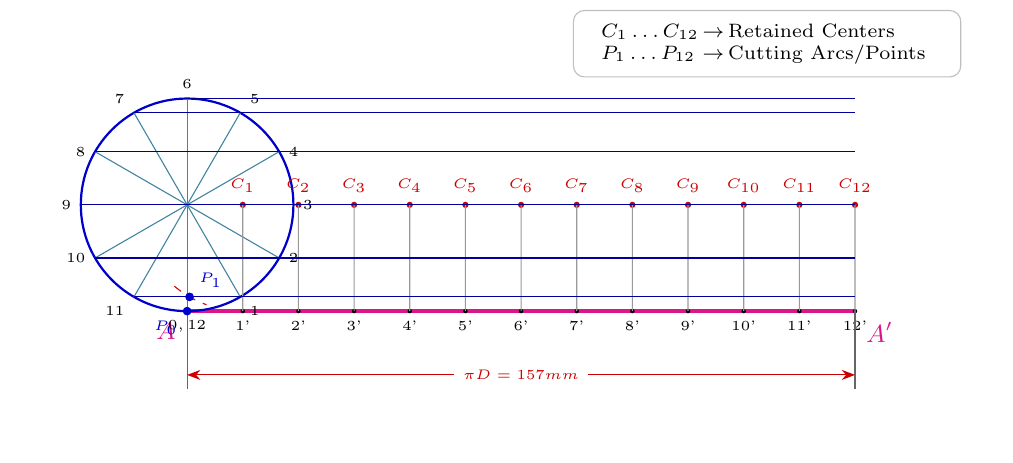
\begin{tikzpicture}[scale=0.45]
  \useasboundingbox (-4.5,-3.5) rectangle (22.5,8.0);
  \drawLegendCard{ \textbf{$C_1\dots C_{12}$} & Retained Centers \\ \textbf{$P_1\dots P_{12}$} & Cutting Arcs/Points }
  \draw[directrix line] (0,0) node[below left] {\small $A$} -- (18.85,0) node[below right] {\small $A'$};
  \draw[axis line] (0,3.0) -- (18.85,3.0);
  \coordinate (C0) at (0,3.0); \draw[thick, blue!80!black] (C0) circle (3.0);
  \draw[thin, construction line] (0,0) -- (C0);
  \draw[thin, cyan!60!black, solid] (C0) -- (0,0);
  \draw[thin, cyan!60!black, solid] (C0) -- ++(300:3.0);
  \draw[thin, cyan!60!black, solid] (C0) -- ++(330:3.0);
  \draw[thin, cyan!60!black, solid] (C0) -- ++(0:3.0);
  \draw[thin, cyan!60!black, solid] (C0) -- ++(30:3.0);
  \draw[thin, cyan!60!black, solid] (C0) -- ++(60:3.0);
  \draw[thin, cyan!60!black, solid] (C0) -- ++(90:3.0);
  \draw[thin, cyan!60!black, solid] (C0) -- ++(120:3.0);
  \draw[thin, cyan!60!black, solid] (C0) -- ++(150:3.0);
  \draw[thin, cyan!60!black, solid] (C0) -- ++(180:3.0);
  \draw[thin, cyan!60!black, solid] (C0) -- ++(210:3.0);
  \draw[thin, cyan!60!black, solid] (C0) -- ++(240:3.0);
  \node[below, font=\tiny] at (0,0) {$0, 12$};
  \node[below right, font=\tiny] at (1.5,0.40) {1};
  \node[right, font=\tiny] at (2.598,1.5) {2};
  \node[right, font=\tiny] at (3.0,3.0) {3};
  \node[right, font=\tiny] at (2.598,4.5) {4};
  \node[above right, font=\tiny] at (1.5,5.598) {5};
  \node[above, font=\tiny] at (0,6.0) {6};
  \node[above left, font=\tiny] at (-1.5,5.598) {7};
  \node[left, font=\tiny] at (-2.598,4.5) {8};
  \node[left, font=\tiny] at (-3.0,3.0) {9};
  \node[left, font=\tiny] at (-2.598,1.5) {10};
  \node[below left, font=\tiny] at (-1.5,0.40) {11};
  \foreach \i in {1,2,...,12} { 
    \fill[black] ({\i*1.5708}, 0) circle (1.8pt);
    \node[below, font=\tiny] at ({\i*1.5708}, 0) {\i'};
    \fill[red!80!black] ({\i*1.5708}, 3.0) circle (2.5pt);
    \node[above=1pt, font=\tiny, red!80!black] at ({\i*1.5708}, 3.0) {$C_{\i}$};
    \coordinate (C\i) at ({\i*1.5708}, 3.0);
    \draw[thin, black!40, solid] ({\i*1.5708}, 0) -- (C\i);
  }
  \draw[dimension extension] (0,0) -- (0,-2.2);
  \draw[dimension extension] (18.85,0) -- (18.85,-2.2);
  \draw[<->, red!80!black, thin] (0,-1.8) -- (18.85,-1.8) node[midway, fill=white] {\tiny $\pi D = 157\text{ mm}$};
  \draw[construction line] (-1.500, 0.402) -- (18.85, 0.402);
  \draw[construction line] (-2.598, 1.500) -- (18.85, 1.500);
  \draw[construction line] (-3.000, 3.000) -- (18.85, 3.000);
  \draw[construction line] (-2.598, 4.500) -- (18.85, 4.500);
  \draw[construction line] (-1.500, 5.598) -- (18.85, 5.598);
  \draw[construction line] (0.000, 6.000) -- (18.85, 6.000);
  \fill[blue!80!black] (0,0) circle (3.5pt) node[below left, font=\tiny] {$P_0$};
  \draw[arc line] (1.5708,3.0) ++(230:3.0) arc (230:250:3.0); \fill[blue!80!black] (0.07, 0.402) circle (3.5pt) node[above right, font=\tiny] {$P_1$};
\end{tikzpicture}
\end{frame}

\begin{frame}{Step 6: Strike Cutting Arcs (Radius = 25 mm) to Locate $P_2$}
\centering
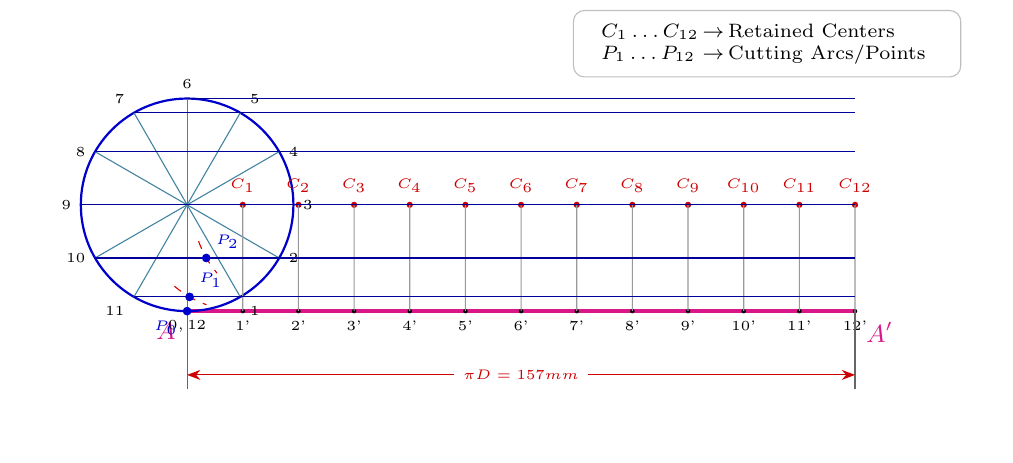
\begin{tikzpicture}[scale=0.45]
  \useasboundingbox (-4.5,-3.5) rectangle (22.5,8.0);
  \drawLegendCard{ \textbf{$C_1\dots C_{12}$} & Retained Centers \\ \textbf{$P_1\dots P_{12}$} & Cutting Arcs/Points }
  \draw[directrix line] (0,0) node[below left] {\small $A$} -- (18.85,0) node[below right] {\small $A'$};
  \draw[axis line] (0,3.0) -- (18.85,3.0);
  \coordinate (C0) at (0,3.0); \draw[thick, blue!80!black] (C0) circle (3.0);
  \draw[thin, construction line] (0,0) -- (C0);
  \draw[thin, cyan!60!black, solid] (C0) -- (0,0);
  \draw[thin, cyan!60!black, solid] (C0) -- ++(300:3.0);
  \draw[thin, cyan!60!black, solid] (C0) -- ++(330:3.0);
  \draw[thin, cyan!60!black, solid] (C0) -- ++(0:3.0);
  \draw[thin, cyan!60!black, solid] (C0) -- ++(30:3.0);
  \draw[thin, cyan!60!black, solid] (C0) -- ++(60:3.0);
  \draw[thin, cyan!60!black, solid] (C0) -- ++(90:3.0);
  \draw[thin, cyan!60!black, solid] (C0) -- ++(120:3.0);
  \draw[thin, cyan!60!black, solid] (C0) -- ++(150:3.0);
  \draw[thin, cyan!60!black, solid] (C0) -- ++(180:3.0);
  \draw[thin, cyan!60!black, solid] (C0) -- ++(210:3.0);
  \draw[thin, cyan!60!black, solid] (C0) -- ++(240:3.0);
  \node[below, font=\tiny] at (0,0) {$0, 12$};
  \node[below right, font=\tiny] at (1.5,0.40) {1};
  \node[right, font=\tiny] at (2.598,1.5) {2};
  \node[right, font=\tiny] at (3.0,3.0) {3};
  \node[right, font=\tiny] at (2.598,4.5) {4};
  \node[above right, font=\tiny] at (1.5,5.598) {5};
  \node[above, font=\tiny] at (0,6.0) {6};
  \node[above left, font=\tiny] at (-1.5,5.598) {7};
  \node[left, font=\tiny] at (-2.598,4.5) {8};
  \node[left, font=\tiny] at (-3.0,3.0) {9};
  \node[left, font=\tiny] at (-2.598,1.5) {10};
  \node[below left, font=\tiny] at (-1.5,0.40) {11};
  \foreach \i in {1,2,...,12} { 
    \fill[black] ({\i*1.5708}, 0) circle (1.8pt);
    \node[below, font=\tiny] at ({\i*1.5708}, 0) {\i'};
    \fill[red!80!black] ({\i*1.5708}, 3.0) circle (2.5pt);
    \node[above=1pt, font=\tiny, red!80!black] at ({\i*1.5708}, 3.0) {$C_{\i}$};
    \coordinate (C\i) at ({\i*1.5708}, 3.0);
    \draw[thin, black!40, solid] ({\i*1.5708}, 0) -- (C\i);
  }
  \draw[dimension extension] (0,0) -- (0,-2.2);
  \draw[dimension extension] (18.85,0) -- (18.85,-2.2);
  \draw[<->, red!80!black, thin] (0,-1.8) -- (18.85,-1.8) node[midway, fill=white] {\tiny $\pi D = 157\text{ mm}$};
  \draw[construction line] (-1.500, 0.402) -- (18.85, 0.402);
  \draw[construction line] (-2.598, 1.500) -- (18.85, 1.500);
  \draw[construction line] (-3.000, 3.000) -- (18.85, 3.000);
  \draw[construction line] (-2.598, 4.500) -- (18.85, 4.500);
  \draw[construction line] (-1.500, 5.598) -- (18.85, 5.598);
  \draw[construction line] (0.000, 6.000) -- (18.85, 6.000);
  \fill[blue!80!black] (0,0) circle (3.5pt) node[below left, font=\tiny] {$P_0$};
  \draw[arc line] (1.5708,3.0) ++(230:3.0) arc (230:250:3.0); \fill[blue!80!black] (0.07, 0.402) circle (3.5pt) node[above right, font=\tiny] {$P_1$};
  \draw[arc line] (3.1416,3.0) ++(200:3.0) arc (200:220:3.0); \fill[blue!80!black] (0.54, 1.500) circle (3.5pt) node[above right, font=\tiny] {$P_2$};
\end{tikzpicture}
\end{frame}

\begin{frame}{Step 6: Strike Cutting Arcs (Radius = 25 mm) to Locate $P_3$}
\centering
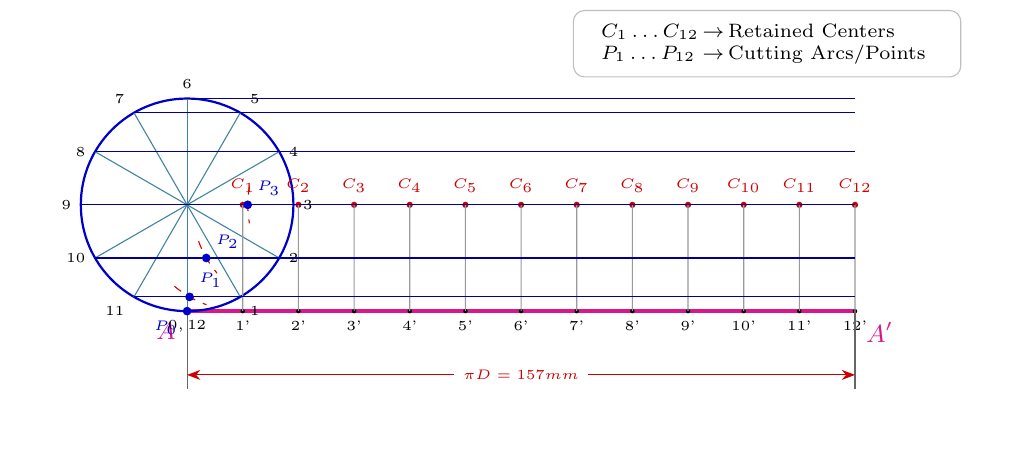
\begin{tikzpicture}[scale=0.45]
  \useasboundingbox (-4.5,-3.5) rectangle (22.5,8.0);
  \drawLegendCard{ \textbf{$C_1\dots C_{12}$} & Retained Centers \\ \textbf{$P_1\dots P_{12}$} & Cutting Arcs/Points }
  \draw[directrix line] (0,0) node[below left] {\small $A$} -- (18.85,0) node[below right] {\small $A'$};
  \draw[axis line] (0,3.0) -- (18.85,3.0);
  \coordinate (C0) at (0,3.0); \draw[thick, blue!80!black] (C0) circle (3.0);
  \draw[thin, construction line] (0,0) -- (C0);
  \draw[thin, cyan!60!black, solid] (C0) -- (0,0);
  \draw[thin, cyan!60!black, solid] (C0) -- ++(300:3.0);
  \draw[thin, cyan!60!black, solid] (C0) -- ++(330:3.0);
  \draw[thin, cyan!60!black, solid] (C0) -- ++(0:3.0);
  \draw[thin, cyan!60!black, solid] (C0) -- ++(30:3.0);
  \draw[thin, cyan!60!black, solid] (C0) -- ++(60:3.0);
  \draw[thin, cyan!60!black, solid] (C0) -- ++(90:3.0);
  \draw[thin, cyan!60!black, solid] (C0) -- ++(120:3.0);
  \draw[thin, cyan!60!black, solid] (C0) -- ++(150:3.0);
  \draw[thin, cyan!60!black, solid] (C0) -- ++(180:3.0);
  \draw[thin, cyan!60!black, solid] (C0) -- ++(210:3.0);
  \draw[thin, cyan!60!black, solid] (C0) -- ++(240:3.0);
  \node[below, font=\tiny] at (0,0) {$0, 12$};
  \node[below right, font=\tiny] at (1.5,0.40) {1};
  \node[right, font=\tiny] at (2.598,1.5) {2};
  \node[right, font=\tiny] at (3.0,3.0) {3};
  \node[right, font=\tiny] at (2.598,4.5) {4};
  \node[above right, font=\tiny] at (1.5,5.598) {5};
  \node[above, font=\tiny] at (0,6.0) {6};
  \node[above left, font=\tiny] at (-1.5,5.598) {7};
  \node[left, font=\tiny] at (-2.598,4.5) {8};
  \node[left, font=\tiny] at (-3.0,3.0) {9};
  \node[left, font=\tiny] at (-2.598,1.5) {10};
  \node[below left, font=\tiny] at (-1.5,0.40) {11};
  \foreach \i in {1,2,...,12} { 
    \fill[black] ({\i*1.5708}, 0) circle (1.8pt);
    \node[below, font=\tiny] at ({\i*1.5708}, 0) {\i'};
    \fill[red!80!black] ({\i*1.5708}, 3.0) circle (2.5pt);
    \node[above=1pt, font=\tiny, red!80!black] at ({\i*1.5708}, 3.0) {$C_{\i}$};
    \coordinate (C\i) at ({\i*1.5708}, 3.0);
    \draw[thin, black!40, solid] ({\i*1.5708}, 0) -- (C\i);
  }
  \draw[dimension extension] (0,0) -- (0,-2.2);
  \draw[dimension extension] (18.85,0) -- (18.85,-2.2);
  \draw[<->, red!80!black, thin] (0,-1.8) -- (18.85,-1.8) node[midway, fill=white] {\tiny $\pi D = 157\text{ mm}$};
  \draw[construction line] (-1.500, 0.402) -- (18.85, 0.402);
  \draw[construction line] (-2.598, 1.500) -- (18.85, 1.500);
  \draw[construction line] (-3.000, 3.000) -- (18.85, 3.000);
  \draw[construction line] (-2.598, 4.500) -- (18.85, 4.500);
  \draw[construction line] (-1.500, 5.598) -- (18.85, 5.598);
  \draw[construction line] (0.000, 6.000) -- (18.85, 6.000);
  \fill[blue!80!black] (0,0) circle (3.5pt) node[below left, font=\tiny] {$P_0$};
  \draw[arc line] (1.5708,3.0) ++(230:3.0) arc (230:250:3.0); \fill[blue!80!black] (0.07, 0.402) circle (3.5pt) node[above right, font=\tiny] {$P_1$};
  \draw[arc line] (3.1416,3.0) ++(200:3.0) arc (200:220:3.0); \fill[blue!80!black] (0.54, 1.500) circle (3.5pt) node[above right, font=\tiny] {$P_2$};
  \draw[arc line] (4.7124,3.0) ++(170:3.0) arc (170:190:3.0); \fill[blue!80!black] (1.71, 3.000) circle (3.5pt) node[above right, font=\tiny] {$P_3$};
\end{tikzpicture}
\end{frame}

\begin{frame}{Step 6: Strike Cutting Arcs (Radius = 25 mm) to Locate $P_4$}
\centering
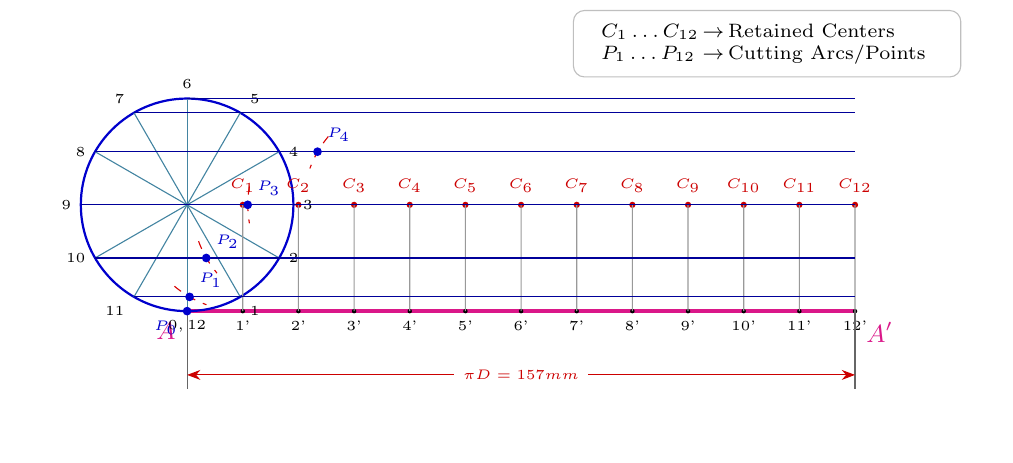
\begin{tikzpicture}[scale=0.45]
  \useasboundingbox (-4.5,-3.5) rectangle (22.5,8.0);
  \drawLegendCard{ \textbf{$C_1\dots C_{12}$} & Retained Centers \\ \textbf{$P_1\dots P_{12}$} & Cutting Arcs/Points }
  \draw[directrix line] (0,0) node[below left] {\small $A$} -- (18.85,0) node[below right] {\small $A'$};
  \draw[axis line] (0,3.0) -- (18.85,3.0);
  \coordinate (C0) at (0,3.0); \draw[thick, blue!80!black] (C0) circle (3.0);
  \draw[thin, construction line] (0,0) -- (C0);
  \draw[thin, cyan!60!black, solid] (C0) -- (0,0);
  \draw[thin, cyan!60!black, solid] (C0) -- ++(300:3.0);
  \draw[thin, cyan!60!black, solid] (C0) -- ++(330:3.0);
  \draw[thin, cyan!60!black, solid] (C0) -- ++(0:3.0);
  \draw[thin, cyan!60!black, solid] (C0) -- ++(30:3.0);
  \draw[thin, cyan!60!black, solid] (C0) -- ++(60:3.0);
  \draw[thin, cyan!60!black, solid] (C0) -- ++(90:3.0);
  \draw[thin, cyan!60!black, solid] (C0) -- ++(120:3.0);
  \draw[thin, cyan!60!black, solid] (C0) -- ++(150:3.0);
  \draw[thin, cyan!60!black, solid] (C0) -- ++(180:3.0);
  \draw[thin, cyan!60!black, solid] (C0) -- ++(210:3.0);
  \draw[thin, cyan!60!black, solid] (C0) -- ++(240:3.0);
  \node[below, font=\tiny] at (0,0) {$0, 12$};
  \node[below right, font=\tiny] at (1.5,0.40) {1};
  \node[right, font=\tiny] at (2.598,1.5) {2};
  \node[right, font=\tiny] at (3.0,3.0) {3};
  \node[right, font=\tiny] at (2.598,4.5) {4};
  \node[above right, font=\tiny] at (1.5,5.598) {5};
  \node[above, font=\tiny] at (0,6.0) {6};
  \node[above left, font=\tiny] at (-1.5,5.598) {7};
  \node[left, font=\tiny] at (-2.598,4.5) {8};
  \node[left, font=\tiny] at (-3.0,3.0) {9};
  \node[left, font=\tiny] at (-2.598,1.5) {10};
  \node[below left, font=\tiny] at (-1.5,0.40) {11};
  \foreach \i in {1,2,...,12} { 
    \fill[black] ({\i*1.5708}, 0) circle (1.8pt);
    \node[below, font=\tiny] at ({\i*1.5708}, 0) {\i'};
    \fill[red!80!black] ({\i*1.5708}, 3.0) circle (2.5pt);
    \node[above=1pt, font=\tiny, red!80!black] at ({\i*1.5708}, 3.0) {$C_{\i}$};
    \coordinate (C\i) at ({\i*1.5708}, 3.0);
    \draw[thin, black!40, solid] ({\i*1.5708}, 0) -- (C\i);
  }
  \draw[dimension extension] (0,0) -- (0,-2.2);
  \draw[dimension extension] (18.85,0) -- (18.85,-2.2);
  \draw[<->, red!80!black, thin] (0,-1.8) -- (18.85,-1.8) node[midway, fill=white] {\tiny $\pi D = 157\text{ mm}$};
  \draw[construction line] (-1.500, 0.402) -- (18.85, 0.402);
  \draw[construction line] (-2.598, 1.500) -- (18.85, 1.500);
  \draw[construction line] (-3.000, 3.000) -- (18.85, 3.000);
  \draw[construction line] (-2.598, 4.500) -- (18.85, 4.500);
  \draw[construction line] (-1.500, 5.598) -- (18.85, 5.598);
  \draw[construction line] (0.000, 6.000) -- (18.85, 6.000);
  \fill[blue!80!black] (0,0) circle (3.5pt) node[below left, font=\tiny] {$P_0$};
  \draw[arc line] (1.5708,3.0) ++(230:3.0) arc (230:250:3.0); \fill[blue!80!black] (0.07, 0.402) circle (3.5pt) node[above right, font=\tiny] {$P_1$};
  \draw[arc line] (3.1416,3.0) ++(200:3.0) arc (200:220:3.0); \fill[blue!80!black] (0.54, 1.500) circle (3.5pt) node[above right, font=\tiny] {$P_2$};
  \draw[arc line] (4.7124,3.0) ++(170:3.0) arc (170:190:3.0); \fill[blue!80!black] (1.71, 3.000) circle (3.5pt) node[above right, font=\tiny] {$P_3$};
  \draw[arc line] (6.2832,3.0) ++(140:3.0) arc (140:160:3.0); \fill[blue!80!black] (3.68, 4.500) circle (3.5pt) node[above right, font=\tiny] {$P_4$};
\end{tikzpicture}
\end{frame}

\begin{frame}{Step 6: Strike Cutting Arcs (Radius = 25 mm) to Locate $P_5$}
\centering
\begin{tikzpicture}[scale=0.45]
  \useasboundingbox (-4.5,-3.5) rectangle (22.5,8.0);
  \drawLegendCard{ \textbf{$C_1\dots C_{12}$} & Retained Centers \\ \textbf{$P_1\dots P_{12}$} & Cutting Arcs/Points }
  \draw[directrix line] (0,0) node[below left] {\small $A$} -- (18.85,0) node[below right] {\small $A'$};
  \draw[axis line] (0,3.0) -- (18.85,3.0);
  \coordinate (C0) at (0,3.0); \draw[thick, blue!80!black] (C0) circle (3.0);
  \draw[thin, construction line] (0,0) -- (C0);
  \draw[thin, cyan!60!black, solid] (C0) -- (0,0);
  \draw[thin, cyan!60!black, solid] (C0) -- ++(300:3.0);
  \draw[thin, cyan!60!black, solid] (C0) -- ++(330:3.0);
  \draw[thin, cyan!60!black, solid] (C0) -- ++(0:3.0);
  \draw[thin, cyan!60!black, solid] (C0) -- ++(30:3.0);
  \draw[thin, cyan!60!black, solid] (C0) -- ++(60:3.0);
  \draw[thin, cyan!60!black, solid] (C0) -- ++(90:3.0);
  \draw[thin, cyan!60!black, solid] (C0) -- ++(120:3.0);
  \draw[thin, cyan!60!black, solid] (C0) -- ++(150:3.0);
  \draw[thin, cyan!60!black, solid] (C0) -- ++(180:3.0);
  \draw[thin, cyan!60!black, solid] (C0) -- ++(210:3.0);
  \draw[thin, cyan!60!black, solid] (C0) -- ++(240:3.0);
  \node[below, font=\tiny] at (0,0) {$0, 12$};
  \node[below right, font=\tiny] at (1.5,0.40) {1};
  \node[right, font=\tiny] at (2.598,1.5) {2};
  \node[right, font=\tiny] at (3.0,3.0) {3};
  \node[right, font=\tiny] at (2.598,4.5) {4};
  \node[above right, font=\tiny] at (1.5,5.598) {5};
  \node[above, font=\tiny] at (0,6.0) {6};
  \node[above left, font=\tiny] at (-1.5,5.598) {7};
  \node[left, font=\tiny] at (-2.598,4.5) {8};
  \node[left, font=\tiny] at (-3.0,3.0) {9};
  \node[left, font=\tiny] at (-2.598,1.5) {10};
  \node[below left, font=\tiny] at (-1.5,0.40) {11};
  \foreach \i in {1,2,...,12} { 
    \fill[black] ({\i*1.5708}, 0) circle (1.8pt);
    \node[below, font=\tiny] at ({\i*1.5708}, 0) {\i'};
    \fill[red!80!black] ({\i*1.5708}, 3.0) circle (2.5pt);
    \node[above=1pt, font=\tiny, red!80!black] at ({\i*1.5708}, 3.0) {$C_{\i}$};
    \coordinate (C\i) at ({\i*1.5708}, 3.0);
    \draw[thin, black!40, solid] ({\i*1.5708}, 0) -- (C\i);
  }
  \draw[dimension extension] (0,0) -- (0,-2.2);
  \draw[dimension extension] (18.85,0) -- (18.85,-2.2);
  \draw[<->, red!80!black, thin] (0,-1.8) -- (18.85,-1.8) node[midway, fill=white] {\tiny $\pi D = 157\text{ mm}$};
  \draw[construction line] (-1.500, 0.402) -- (18.85, 0.402);
  \draw[construction line] (-2.598, 1.500) -- (18.85, 1.500);
  \draw[construction line] (-3.000, 3.000) -- (18.85, 3.000);
  \draw[construction line] (-2.598, 4.500) -- (18.85, 4.500);
  \draw[construction line] (-1.500, 5.598) -- (18.85, 5.598);
  \draw[construction line] (0.000, 6.000) -- (18.85, 6.000);
  \fill[blue!80!black] (0,0) circle (3.5pt) node[below left, font=\tiny] {$P_0$};
  \draw[arc line] (1.5708,3.0) ++(230:3.0) arc (230:250:3.0); \fill[blue!80!black] (0.07, 0.402) circle (3.5pt) node[above right, font=\tiny] {$P_1$};
  \draw[arc line] (3.1416,3.0) ++(200:3.0) arc (200:220:3.0); \fill[blue!80!black] (0.54, 1.500) circle (3.5pt) node[above right, font=\tiny] {$P_2$};
  \draw[arc line] (4.7124,3.0) ++(170:3.0) arc (170:190:3.0); \fill[blue!80!black] (1.71, 3.000) circle (3.5pt) node[above right, font=\tiny] {$P_3$};
  \draw[arc line] (6.2832,3.0) ++(140:3.0) arc (140:160:3.0); \fill[blue!80!black] (3.68, 4.500) circle (3.5pt) node[above right, font=\tiny] {$P_4$};
  \draw[arc line] (7.8540,3.0) ++(110:3.0) arc (110:130:3.0); \fill[blue!80!black] (6.42, 5.598) circle (3.5pt) node[above right, font=\tiny] {$P_5$};
\end{tikzpicture}
\end{frame}

\begin{frame}{Step 6: Strike Cutting Arcs (Radius = 25 mm) to Locate $P_6$}
\centering
\begin{tikzpicture}[scale=0.45]
  \useasboundingbox (-4.5,-3.5) rectangle (22.5,8.0);
  \drawLegendCard{ \textbf{$C_1\dots C_{12}$} & Retained Centers \\ \textbf{$P_1\dots P_{12}$} & Cutting Arcs/Points }
  \draw[directrix line] (0,0) node[below left] {\small $A$} -- (18.85,0) node[below right] {\small $A'$};
  \draw[axis line] (0,3.0) -- (18.85,3.0);
  \coordinate (C0) at (0,3.0); \draw[thick, blue!80!black] (C0) circle (3.0);
  \draw[thin, construction line] (0,0) -- (C0);
  \draw[thin, cyan!60!black, solid] (C0) -- (0,0);
  \draw[thin, cyan!60!black, solid] (C0) -- ++(300:3.0);
  \draw[thin, cyan!60!black, solid] (C0) -- ++(330:3.0);
  \draw[thin, cyan!60!black, solid] (C0) -- ++(0:3.0);
  \draw[thin, cyan!60!black, solid] (C0) -- ++(30:3.0);
  \draw[thin, cyan!60!black, solid] (C0) -- ++(60:3.0);
  \draw[thin, cyan!60!black, solid] (C0) -- ++(90:3.0);
  \draw[thin, cyan!60!black, solid] (C0) -- ++(120:3.0);
  \draw[thin, cyan!60!black, solid] (C0) -- ++(150:3.0);
  \draw[thin, cyan!60!black, solid] (C0) -- ++(180:3.0);
  \draw[thin, cyan!60!black, solid] (C0) -- ++(210:3.0);
  \draw[thin, cyan!60!black, solid] (C0) -- ++(240:3.0);
  \node[below, font=\tiny] at (0,0) {$0, 12$};
  \node[below right, font=\tiny] at (1.5,0.40) {1};
  \node[right, font=\tiny] at (2.598,1.5) {2};
  \node[right, font=\tiny] at (3.0,3.0) {3};
  \node[right, font=\tiny] at (2.598,4.5) {4};
  \node[above right, font=\tiny] at (1.5,5.598) {5};
  \node[above, font=\tiny] at (0,6.0) {6};
  \node[above left, font=\tiny] at (-1.5,5.598) {7};
  \node[left, font=\tiny] at (-2.598,4.5) {8};
  \node[left, font=\tiny] at (-3.0,3.0) {9};
  \node[left, font=\tiny] at (-2.598,1.5) {10};
  \node[below left, font=\tiny] at (-1.5,0.40) {11};
  \foreach \i in {1,2,...,12} { 
    \fill[black] ({\i*1.5708}, 0) circle (1.8pt);
    \node[below, font=\tiny] at ({\i*1.5708}, 0) {\i'};
    \fill[red!80!black] ({\i*1.5708}, 3.0) circle (2.5pt);
    \node[above=1pt, font=\tiny, red!80!black] at ({\i*1.5708}, 3.0) {$C_{\i}$};
    \coordinate (C\i) at ({\i*1.5708}, 3.0);
    \draw[thin, black!40, solid] ({\i*1.5708}, 0) -- (C\i);
  }
  \draw[dimension extension] (0,0) -- (0,-2.2);
  \draw[dimension extension] (18.85,0) -- (18.85,-2.2);
  \draw[<->, red!80!black, thin] (0,-1.8) -- (18.85,-1.8) node[midway, fill=white] {\tiny $\pi D = 157\text{ mm}$};
  \draw[construction line] (-1.500, 0.402) -- (18.85, 0.402);
  \draw[construction line] (-2.598, 1.500) -- (18.85, 1.500);
  \draw[construction line] (-3.000, 3.000) -- (18.85, 3.000);
  \draw[construction line] (-2.598, 4.500) -- (18.85, 4.500);
  \draw[construction line] (-1.500, 5.598) -- (18.85, 5.598);
  \draw[construction line] (0.000, 6.000) -- (18.85, 6.000);
  \fill[blue!80!black] (0,0) circle (3.5pt) node[below left, font=\tiny] {$P_0$};
  \draw[arc line] (1.5708,3.0) ++(230:3.0) arc (230:250:3.0); \fill[blue!80!black] (0.07, 0.402) circle (3.5pt) node[above right, font=\tiny] {$P_1$};
  \draw[arc line] (3.1416,3.0) ++(200:3.0) arc (200:220:3.0); \fill[blue!80!black] (0.54, 1.500) circle (3.5pt) node[above right, font=\tiny] {$P_2$};
  \draw[arc line] (4.7124,3.0) ++(170:3.0) arc (170:190:3.0); \fill[blue!80!black] (1.71, 3.000) circle (3.5pt) node[above right, font=\tiny] {$P_3$};
  \draw[arc line] (6.2832,3.0) ++(140:3.0) arc (140:160:3.0); \fill[blue!80!black] (3.68, 4.500) circle (3.5pt) node[above right, font=\tiny] {$P_4$};
  \draw[arc line] (7.8540,3.0) ++(110:3.0) arc (110:130:3.0); \fill[blue!80!black] (6.42, 5.598) circle (3.5pt) node[above right, font=\tiny] {$P_5$};
  \draw[arc line] (9.4248,3.0) ++(80:3.0) arc (80:100:3.0); \fill[blue!80!black] (9.42, 6.000) circle (3.5pt) node[above, font=\tiny] {$P_6$};
\end{tikzpicture}
\end{frame}

\begin{frame}{Step 6: Strike Cutting Arcs (Radius = 25 mm) to Locate $P_7$}
\centering
\begin{tikzpicture}[scale=0.45]
  \useasboundingbox (-4.5,-3.5) rectangle (22.5,8.0);
  \drawLegendCard{ \textbf{$C_1\dots C_{12}$} & Retained Centers \\ \textbf{$P_1\dots P_{12}$} & Cutting Arcs/Points }
  \draw[directrix line] (0,0) node[below left] {\small $A$} -- (18.85,0) node[below right] {\small $A'$};
  \draw[axis line] (0,3.0) -- (18.85,3.0);
  \coordinate (C0) at (0,3.0); \draw[thick, blue!80!black] (C0) circle (3.0);
  \draw[thin, construction line] (0,0) -- (C0);
  \draw[thin, cyan!60!black, solid] (C0) -- (0,0);
  \draw[thin, cyan!60!black, solid] (C0) -- ++(300:3.0);
  \draw[thin, cyan!60!black, solid] (C0) -- ++(330:3.0);
  \draw[thin, cyan!60!black, solid] (C0) -- ++(0:3.0);
  \draw[thin, cyan!60!black, solid] (C0) -- ++(30:3.0);
  \draw[thin, cyan!60!black, solid] (C0) -- ++(60:3.0);
  \draw[thin, cyan!60!black, solid] (C0) -- ++(90:3.0);
  \draw[thin, cyan!60!black, solid] (C0) -- ++(120:3.0);
  \draw[thin, cyan!60!black, solid] (C0) -- ++(150:3.0);
  \draw[thin, cyan!60!black, solid] (C0) -- ++(180:3.0);
  \draw[thin, cyan!60!black, solid] (C0) -- ++(210:3.0);
  \draw[thin, cyan!60!black, solid] (C0) -- ++(240:3.0);
  \node[below, font=\tiny] at (0,0) {$0, 12$};
  \node[below right, font=\tiny] at (1.5,0.40) {1};
  \node[right, font=\tiny] at (2.598,1.5) {2};
  \node[right, font=\tiny] at (3.0,3.0) {3};
  \node[right, font=\tiny] at (2.598,4.5) {4};
  \node[above right, font=\tiny] at (1.5,5.598) {5};
  \node[above, font=\tiny] at (0,6.0) {6};
  \node[above left, font=\tiny] at (-1.5,5.598) {7};
  \node[left, font=\tiny] at (-2.598,4.5) {8};
  \node[left, font=\tiny] at (-3.0,3.0) {9};
  \node[left, font=\tiny] at (-2.598,1.5) {10};
  \node[below left, font=\tiny] at (-1.5,0.40) {11};
  \foreach \i in {1,2,...,12} { 
    \fill[black] ({\i*1.5708}, 0) circle (1.8pt);
    \node[below, font=\tiny] at ({\i*1.5708}, 0) {\i'};
    \fill[red!80!black] ({\i*1.5708}, 3.0) circle (2.5pt);
    \node[above=1pt, font=\tiny, red!80!black] at ({\i*1.5708}, 3.0) {$C_{\i}$};
    \coordinate (C\i) at ({\i*1.5708}, 3.0);
    \draw[thin, black!40, solid] ({\i*1.5708}, 0) -- (C\i);
  }
  \draw[dimension extension] (0,0) -- (0,-2.2);
  \draw[dimension extension] (18.85,0) -- (18.85,-2.2);
  \draw[<->, red!80!black, thin] (0,-1.8) -- (18.85,-1.8) node[midway, fill=white] {\tiny $\pi D = 157\text{ mm}$};
  \draw[construction line] (-1.500, 0.402) -- (18.85, 0.402);
  \draw[construction line] (-2.598, 1.500) -- (18.85, 1.500);
  \draw[construction line] (-3.000, 3.000) -- (18.85, 3.000);
  \draw[construction line] (-2.598, 4.500) -- (18.85, 4.500);
  \draw[construction line] (-1.500, 5.598) -- (18.85, 5.598);
  \draw[construction line] (0.000, 6.000) -- (18.85, 6.000);
  \fill[blue!80!black] (0,0) circle (3.5pt) node[below left, font=\tiny] {$P_0$};
  \draw[arc line] (1.5708,3.0) ++(230:3.0) arc (230:250:3.0); \fill[blue!80!black] (0.07, 0.402) circle (3.5pt) node[above right, font=\tiny] {$P_1$};
  \draw[arc line] (3.1416,3.0) ++(200:3.0) arc (200:220:3.0); \fill[blue!80!black] (0.54, 1.500) circle (3.5pt) node[above right, font=\tiny] {$P_2$};
  \draw[arc line] (4.7124,3.0) ++(170:3.0) arc (170:190:3.0); \fill[blue!80!black] (1.71, 3.000) circle (3.5pt) node[above right, font=\tiny] {$P_3$};
  \draw[arc line] (6.2832,3.0) ++(140:3.0) arc (140:160:3.0); \fill[blue!80!black] (3.68, 4.500) circle (3.5pt) node[above right, font=\tiny] {$P_4$};
  \draw[arc line] (7.8540,3.0) ++(110:3.0) arc (110:130:3.0); \fill[blue!80!black] (6.42, 5.598) circle (3.5pt) node[above right, font=\tiny] {$P_5$};
  \draw[arc line] (9.4248,3.0) ++(80:3.0) arc (80:100:3.0); \fill[blue!80!black] (9.42, 6.000) circle (3.5pt) node[above, font=\tiny] {$P_6$};
  \draw[arc line] (10.9956,3.0) ++(50:3.0) arc (50:70:3.0); \fill[blue!80!black] (12.42, 5.598) circle (3.5pt) node[above left, font=\tiny] {$P_7$};
\end{tikzpicture}
\end{frame}

\begin{frame}{Step 6: Strike Cutting Arcs (Radius = 25 mm) to Locate $P_8$}
\centering
\begin{tikzpicture}[scale=0.45]
  \useasboundingbox (-4.5,-3.5) rectangle (22.5,8.0);
  \drawLegendCard{ \textbf{$C_1\dots C_{12}$} & Retained Centers \\ \textbf{$P_1\dots P_{12}$} & Cutting Arcs/Points }
  \draw[directrix line] (0,0) node[below left] {\small $A$} -- (18.85,0) node[below right] {\small $A'$};
  \draw[axis line] (0,3.0) -- (18.85,3.0);
  \coordinate (C0) at (0,3.0); \draw[thick, blue!80!black] (C0) circle (3.0);
  \draw[thin, construction line] (0,0) -- (C0);
  \draw[thin, cyan!60!black, solid] (C0) -- (0,0);
  \draw[thin, cyan!60!black, solid] (C0) -- ++(300:3.0);
  \draw[thin, cyan!60!black, solid] (C0) -- ++(330:3.0);
  \draw[thin, cyan!60!black, solid] (C0) -- ++(0:3.0);
  \draw[thin, cyan!60!black, solid] (C0) -- ++(30:3.0);
  \draw[thin, cyan!60!black, solid] (C0) -- ++(60:3.0);
  \draw[thin, cyan!60!black, solid] (C0) -- ++(90:3.0);
  \draw[thin, cyan!60!black, solid] (C0) -- ++(120:3.0);
  \draw[thin, cyan!60!black, solid] (C0) -- ++(150:3.0);
  \draw[thin, cyan!60!black, solid] (C0) -- ++(180:3.0);
  \draw[thin, cyan!60!black, solid] (C0) -- ++(210:3.0);
  \draw[thin, cyan!60!black, solid] (C0) -- ++(240:3.0);
  \node[below, font=\tiny] at (0,0) {$0, 12$};
  \node[below right, font=\tiny] at (1.5,0.40) {1};
  \node[right, font=\tiny] at (2.598,1.5) {2};
  \node[right, font=\tiny] at (3.0,3.0) {3};
  \node[right, font=\tiny] at (2.598,4.5) {4};
  \node[above right, font=\tiny] at (1.5,5.598) {5};
  \node[above, font=\tiny] at (0,6.0) {6};
  \node[above left, font=\tiny] at (-1.5,5.598) {7};
  \node[left, font=\tiny] at (-2.598,4.5) {8};
  \node[left, font=\tiny] at (-3.0,3.0) {9};
  \node[left, font=\tiny] at (-2.598,1.5) {10};
  \node[below left, font=\tiny] at (-1.5,0.40) {11};
  \foreach \i in {1,2,...,12} { 
    \fill[black] ({\i*1.5708}, 0) circle (1.8pt);
    \node[below, font=\tiny] at ({\i*1.5708}, 0) {\i'};
    \fill[red!80!black] ({\i*1.5708}, 3.0) circle (2.5pt);
    \node[above=1pt, font=\tiny, red!80!black] at ({\i*1.5708}, 3.0) {$C_{\i}$};
    \coordinate (C\i) at ({\i*1.5708}, 3.0);
    \draw[thin, black!40, solid] ({\i*1.5708}, 0) -- (C\i);
  }
  \draw[dimension extension] (0,0) -- (0,-2.2);
  \draw[dimension extension] (18.85,0) -- (18.85,-2.2);
  \draw[<->, red!80!black, thin] (0,-1.8) -- (18.85,-1.8) node[midway, fill=white] {\tiny $\pi D = 157\text{ mm}$};
  \draw[construction line] (-1.500, 0.402) -- (18.85, 0.402);
  \draw[construction line] (-2.598, 1.500) -- (18.85, 1.500);
  \draw[construction line] (-3.000, 3.000) -- (18.85, 3.000);
  \draw[construction line] (-2.598, 4.500) -- (18.85, 4.500);
  \draw[construction line] (-1.500, 5.598) -- (18.85, 5.598);
  \draw[construction line] (0.000, 6.000) -- (18.85, 6.000);
  \fill[blue!80!black] (0,0) circle (3.5pt) node[below left, font=\tiny] {$P_0$};
  \draw[arc line] (1.5708,3.0) ++(230:3.0) arc (230:250:3.0); \fill[blue!80!black] (0.07, 0.402) circle (3.5pt) node[above right, font=\tiny] {$P_1$};
  \draw[arc line] (3.1416,3.0) ++(200:3.0) arc (200:220:3.0); \fill[blue!80!black] (0.54, 1.500) circle (3.5pt) node[above right, font=\tiny] {$P_2$};
  \draw[arc line] (4.7124,3.0) ++(170:3.0) arc (170:190:3.0); \fill[blue!80!black] (1.71, 3.000) circle (3.5pt) node[above right, font=\tiny] {$P_3$};
  \draw[arc line] (6.2832,3.0) ++(140:3.0) arc (140:160:3.0); \fill[blue!80!black] (3.68, 4.500) circle (3.5pt) node[above right, font=\tiny] {$P_4$};
  \draw[arc line] (7.8540,3.0) ++(110:3.0) arc (110:130:3.0); \fill[blue!80!black] (6.42, 5.598) circle (3.5pt) node[above right, font=\tiny] {$P_5$};
  \draw[arc line] (9.4248,3.0) ++(80:3.0) arc (80:100:3.0); \fill[blue!80!black] (9.42, 6.000) circle (3.5pt) node[above, font=\tiny] {$P_6$};
  \draw[arc line] (10.9956,3.0) ++(50:3.0) arc (50:70:3.0); \fill[blue!80!black] (12.42, 5.598) circle (3.5pt) node[above left, font=\tiny] {$P_7$};
  \draw[arc line] (12.5664,3.0) ++(20:3.0) arc (20:40:3.0); \fill[blue!80!black] (15.17, 4.500) circle (3.5pt) node[above left, font=\tiny] {$P_8$};
\end{tikzpicture}
\end{frame}

\begin{frame}{Step 6: Strike Cutting Arcs (Radius = 25 mm) to Locate $P_9$}
\centering
\begin{tikzpicture}[scale=0.45]
  \useasboundingbox (-4.5,-3.5) rectangle (22.5,8.0);
  \drawLegendCard{ \textbf{$C_1\dots C_{12}$} & Retained Centers \\ \textbf{$P_1\dots P_{12}$} & Cutting Arcs/Points }
  \draw[directrix line] (0,0) node[below left] {\small $A$} -- (18.85,0) node[below right] {\small $A'$};
  \draw[axis line] (0,3.0) -- (18.85,3.0);
  \coordinate (C0) at (0,3.0); \draw[thick, blue!80!black] (C0) circle (3.0);
  \draw[thin, construction line] (0,0) -- (C0);
  \draw[thin, cyan!60!black, solid] (C0) -- (0,0);
  \draw[thin, cyan!60!black, solid] (C0) -- ++(300:3.0);
  \draw[thin, cyan!60!black, solid] (C0) -- ++(330:3.0);
  \draw[thin, cyan!60!black, solid] (C0) -- ++(0:3.0);
  \draw[thin, cyan!60!black, solid] (C0) -- ++(30:3.0);
  \draw[thin, cyan!60!black, solid] (C0) -- ++(60:3.0);
  \draw[thin, cyan!60!black, solid] (C0) -- ++(90:3.0);
  \draw[thin, cyan!60!black, solid] (C0) -- ++(120:3.0);
  \draw[thin, cyan!60!black, solid] (C0) -- ++(150:3.0);
  \draw[thin, cyan!60!black, solid] (C0) -- ++(180:3.0);
  \draw[thin, cyan!60!black, solid] (C0) -- ++(210:3.0);
  \draw[thin, cyan!60!black, solid] (C0) -- ++(240:3.0);
  \node[below, font=\tiny] at (0,0) {$0, 12$};
  \node[below right, font=\tiny] at (1.5,0.40) {1};
  \node[right, font=\tiny] at (2.598,1.5) {2};
  \node[right, font=\tiny] at (3.0,3.0) {3};
  \node[right, font=\tiny] at (2.598,4.5) {4};
  \node[above right, font=\tiny] at (1.5,5.598) {5};
  \node[above, font=\tiny] at (0,6.0) {6};
  \node[above left, font=\tiny] at (-1.5,5.598) {7};
  \node[left, font=\tiny] at (-2.598,4.5) {8};
  \node[left, font=\tiny] at (-3.0,3.0) {9};
  \node[left, font=\tiny] at (-2.598,1.5) {10};
  \node[below left, font=\tiny] at (-1.5,0.40) {11};
  \foreach \i in {1,2,...,12} { 
    \fill[black] ({\i*1.5708}, 0) circle (1.8pt);
    \node[below, font=\tiny] at ({\i*1.5708}, 0) {\i'};
    \fill[red!80!black] ({\i*1.5708}, 3.0) circle (2.5pt);
    \node[above=1pt, font=\tiny, red!80!black] at ({\i*1.5708}, 3.0) {$C_{\i}$};
    \coordinate (C\i) at ({\i*1.5708}, 3.0);
    \draw[thin, black!40, solid] ({\i*1.5708}, 0) -- (C\i);
  }
  \draw[dimension extension] (0,0) -- (0,-2.2);
  \draw[dimension extension] (18.85,0) -- (18.85,-2.2);
  \draw[<->, red!80!black, thin] (0,-1.8) -- (18.85,-1.8) node[midway, fill=white] {\tiny $\pi D = 157\text{ mm}$};
  \draw[construction line] (-1.500, 0.402) -- (18.85, 0.402);
  \draw[construction line] (-2.598, 1.500) -- (18.85, 1.500);
  \draw[construction line] (-3.000, 3.000) -- (18.85, 3.000);
  \draw[construction line] (-2.598, 4.500) -- (18.85, 4.500);
  \draw[construction line] (-1.500, 5.598) -- (18.85, 5.598);
  \draw[construction line] (0.000, 6.000) -- (18.85, 6.000);
  \fill[blue!80!black] (0,0) circle (3.5pt) node[below left, font=\tiny] {$P_0$};
  \draw[arc line] (1.5708,3.0) ++(230:3.0) arc (230:250:3.0); \fill[blue!80!black] (0.07, 0.402) circle (3.5pt) node[above right, font=\tiny] {$P_1$};
  \draw[arc line] (3.1416,3.0) ++(200:3.0) arc (200:220:3.0); \fill[blue!80!black] (0.54, 1.500) circle (3.5pt) node[above right, font=\tiny] {$P_2$};
  \draw[arc line] (4.7124,3.0) ++(170:3.0) arc (170:190:3.0); \fill[blue!80!black] (1.71, 3.000) circle (3.5pt) node[above right, font=\tiny] {$P_3$};
  \draw[arc line] (6.2832,3.0) ++(140:3.0) arc (140:160:3.0); \fill[blue!80!black] (3.68, 4.500) circle (3.5pt) node[above right, font=\tiny] {$P_4$};
  \draw[arc line] (7.8540,3.0) ++(110:3.0) arc (110:130:3.0); \fill[blue!80!black] (6.42, 5.598) circle (3.5pt) node[above right, font=\tiny] {$P_5$};
  \draw[arc line] (9.4248,3.0) ++(80:3.0) arc (80:100:3.0); \fill[blue!80!black] (9.42, 6.000) circle (3.5pt) node[above, font=\tiny] {$P_6$};
  \draw[arc line] (10.9956,3.0) ++(50:3.0) arc (50:70:3.0); \fill[blue!80!black] (12.42, 5.598) circle (3.5pt) node[above left, font=\tiny] {$P_7$};
  \draw[arc line] (12.5664,3.0) ++(20:3.0) arc (20:40:3.0); \fill[blue!80!black] (15.17, 4.500) circle (3.5pt) node[above left, font=\tiny] {$P_8$};
  \draw[arc line] (14.1372,3.0) ++(350:3.0) arc (350:10:3.0); \fill[blue!80!black] (17.14, 3.000) circle (3.5pt) node[above left, font=\tiny] {$P_9$};
\end{tikzpicture}
\end{frame}

\begin{frame}{Step 6: Strike Cutting Arcs (Radius = 25 mm) to Locate $P_{10}$}
\centering
\begin{tikzpicture}[scale=0.45]
  \useasboundingbox (-4.5,-3.5) rectangle (22.5,8.0);
  \drawLegendCard{ \textbf{$C_1\dots C_{12}$} & Retained Centers \\ \textbf{$P_1\dots P_{12}$} & Cutting Arcs/Points }
  \draw[directrix line] (0,0) node[below left] {\small $A$} -- (18.85,0) node[below right] {\small $A'$};
  \draw[axis line] (0,3.0) -- (18.85,3.0);
  \coordinate (C0) at (0,3.0); \draw[thick, blue!80!black] (C0) circle (3.0);
  \draw[thin, construction line] (0,0) -- (C0);
  \draw[thin, cyan!60!black, solid] (C0) -- (0,0);
  \draw[thin, cyan!60!black, solid] (C0) -- ++(300:3.0);
  \draw[thin, cyan!60!black, solid] (C0) -- ++(330:3.0);
  \draw[thin, cyan!60!black, solid] (C0) -- ++(0:3.0);
  \draw[thin, cyan!60!black, solid] (C0) -- ++(30:3.0);
  \draw[thin, cyan!60!black, solid] (C0) -- ++(60:3.0);
  \draw[thin, cyan!60!black, solid] (C0) -- ++(90:3.0);
  \draw[thin, cyan!60!black, solid] (C0) -- ++(120:3.0);
  \draw[thin, cyan!60!black, solid] (C0) -- ++(150:3.0);
  \draw[thin, cyan!60!black, solid] (C0) -- ++(180:3.0);
  \draw[thin, cyan!60!black, solid] (C0) -- ++(210:3.0);
  \draw[thin, cyan!60!black, solid] (C0) -- ++(240:3.0);
  \node[below, font=\tiny] at (0,0) {$0, 12$};
  \node[below right, font=\tiny] at (1.5,0.40) {1};
  \node[right, font=\tiny] at (2.598,1.5) {2};
  \node[right, font=\tiny] at (3.0,3.0) {3};
  \node[right, font=\tiny] at (2.598,4.5) {4};
  \node[above right, font=\tiny] at (1.5,5.598) {5};
  \node[above, font=\tiny] at (0,6.0) {6};
  \node[above left, font=\tiny] at (-1.5,5.598) {7};
  \node[left, font=\tiny] at (-2.598,4.5) {8};
  \node[left, font=\tiny] at (-3.0,3.0) {9};
  \node[left, font=\tiny] at (-2.598,1.5) {10};
  \node[below left, font=\tiny] at (-1.5,0.40) {11};
  \foreach \i in {1,2,...,12} { 
    \fill[black] ({\i*1.5708}, 0) circle (1.8pt);
    \node[below, font=\tiny] at ({\i*1.5708}, 0) {\i'};
    \fill[red!80!black] ({\i*1.5708}, 3.0) circle (2.5pt);
    \node[above=1pt, font=\tiny, red!80!black] at ({\i*1.5708}, 3.0) {$C_{\i}$};
    \coordinate (C\i) at ({\i*1.5708}, 3.0);
    \draw[thin, black!40, solid] ({\i*1.5708}, 0) -- (C\i);
  }
  \draw[dimension extension] (0,0) -- (0,-2.2);
  \draw[dimension extension] (18.85,0) -- (18.85,-2.2);
  \draw[<->, red!80!black, thin] (0,-1.8) -- (18.85,-1.8) node[midway, fill=white] {\tiny $\pi D = 157\text{ mm}$};
  \draw[construction line] (-1.500, 0.402) -- (18.85, 0.402);
  \draw[construction line] (-2.598, 1.500) -- (18.85, 1.500);
  \draw[construction line] (-3.000, 3.000) -- (18.85, 3.000);
  \draw[construction line] (-2.598, 4.500) -- (18.85, 4.500);
  \draw[construction line] (-1.500, 5.598) -- (18.85, 5.598);
  \draw[construction line] (0.000, 6.000) -- (18.85, 6.000);
  \fill[blue!80!black] (0,0) circle (3.5pt) node[below left, font=\tiny] {$P_0$};
  \draw[arc line] (1.5708,3.0) ++(230:3.0) arc (230:250:3.0); \fill[blue!80!black] (0.07, 0.402) circle (3.5pt) node[above right, font=\tiny] {$P_1$};
  \draw[arc line] (3.1416,3.0) ++(200:3.0) arc (200:220:3.0); \fill[blue!80!black] (0.54, 1.500) circle (3.5pt) node[above right, font=\tiny] {$P_2$};
  \draw[arc line] (4.7124,3.0) ++(170:3.0) arc (170:190:3.0); \fill[blue!80!black] (1.71, 3.000) circle (3.5pt) node[above right, font=\tiny] {$P_3$};
  \draw[arc line] (6.2832,3.0) ++(140:3.0) arc (140:160:3.0); \fill[blue!80!black] (3.68, 4.500) circle (3.5pt) node[above right, font=\tiny] {$P_4$};
  \draw[arc line] (7.8540,3.0) ++(110:3.0) arc (110:130:3.0); \fill[blue!80!black] (6.42, 5.598) circle (3.5pt) node[above right, font=\tiny] {$P_5$};
  \draw[arc line] (9.4248,3.0) ++(80:3.0) arc (80:100:3.0); \fill[blue!80!black] (9.42, 6.000) circle (3.5pt) node[above, font=\tiny] {$P_6$};
  \draw[arc line] (10.9956,3.0) ++(50:3.0) arc (50:70:3.0); \fill[blue!80!black] (12.42, 5.598) circle (3.5pt) node[above left, font=\tiny] {$P_7$};
  \draw[arc line] (12.5664,3.0) ++(20:3.0) arc (20:40:3.0); \fill[blue!80!black] (15.17, 4.500) circle (3.5pt) node[above left, font=\tiny] {$P_8$};
  \draw[arc line] (14.1372,3.0) ++(350:3.0) arc (350:10:3.0); \fill[blue!80!black] (17.14, 3.000) circle (3.5pt) node[above left, font=\tiny] {$P_9$};
  \draw[arc line] (15.7080,3.0) ++(320:3.0) arc (320:340:3.0); \fill[blue!80!black] (18.31, 1.500) circle (3.5pt) node[above left, font=\tiny] {$P_{10}$};
\end{tikzpicture}
\end{frame}

\begin{frame}{Step 6: Strike Cutting Arcs (Radius = 25 mm) to Locate $P_{11}$}
\centering
\begin{tikzpicture}[scale=0.45]
  \useasboundingbox (-4.5,-3.5) rectangle (22.5,8.0);
  \drawLegendCard{ \textbf{$C_1\dots C_{12}$} & Retained Centers \\ \textbf{$P_1\dots P_{12}$} & Cutting Arcs/Points }
  \draw[directrix line] (0,0) node[below left] {\small $A$} -- (18.85,0) node[below right] {\small $A'$};
  \draw[axis line] (0,3.0) -- (18.85,3.0);
  \coordinate (C0) at (0,3.0); \draw[thick, blue!80!black] (C0) circle (3.0);
  \draw[thin, construction line] (0,0) -- (C0);
  \draw[thin, cyan!60!black, solid] (C0) -- (0,0);
  \draw[thin, cyan!60!black, solid] (C0) -- ++(300:3.0);
  \draw[thin, cyan!60!black, solid] (C0) -- ++(330:3.0);
  \draw[thin, cyan!60!black, solid] (C0) -- ++(0:3.0);
  \draw[thin, cyan!60!black, solid] (C0) -- ++(30:3.0);
  \draw[thin, cyan!60!black, solid] (C0) -- ++(60:3.0);
  \draw[thin, cyan!60!black, solid] (C0) -- ++(90:3.0);
  \draw[thin, cyan!60!black, solid] (C0) -- ++(120:3.0);
  \draw[thin, cyan!60!black, solid] (C0) -- ++(150:3.0);
  \draw[thin, cyan!60!black, solid] (C0) -- ++(180:3.0);
  \draw[thin, cyan!60!black, solid] (C0) -- ++(210:3.0);
  \draw[thin, cyan!60!black, solid] (C0) -- ++(240:3.0);
  \node[below, font=\tiny] at (0,0) {$0, 12$};
  \node[below right, font=\tiny] at (1.5,0.40) {1};
  \node[right, font=\tiny] at (2.598,1.5) {2};
  \node[right, font=\tiny] at (3.0,3.0) {3};
  \node[right, font=\tiny] at (2.598,4.5) {4};
  \node[above right, font=\tiny] at (1.5,5.598) {5};
  \node[above, font=\tiny] at (0,6.0) {6};
  \node[above left, font=\tiny] at (-1.5,5.598) {7};
  \node[left, font=\tiny] at (-2.598,4.5) {8};
  \node[left, font=\tiny] at (-3.0,3.0) {9};
  \node[left, font=\tiny] at (-2.598,1.5) {10};
  \node[below left, font=\tiny] at (-1.5,0.40) {11};
  \foreach \i in {1,2,...,12} { 
    \fill[black] ({\i*1.5708}, 0) circle (1.8pt);
    \node[below, font=\tiny] at ({\i*1.5708}, 0) {\i'};
    \fill[red!80!black] ({\i*1.5708}, 3.0) circle (2.5pt);
    \node[above=1pt, font=\tiny, red!80!black] at ({\i*1.5708}, 3.0) {$C_{\i}$};
    \coordinate (C\i) at ({\i*1.5708}, 3.0);
    \draw[thin, black!40, solid] ({\i*1.5708}, 0) -- (C\i);
  }
  \draw[dimension extension] (0,0) -- (0,-2.2);
  \draw[dimension extension] (18.85,0) -- (18.85,-2.2);
  \draw[<->, red!80!black, thin] (0,-1.8) -- (18.85,-1.8) node[midway, fill=white] {\tiny $\pi D = 157\text{ mm}$};
  \draw[construction line] (-1.500, 0.402) -- (18.85, 0.402);
  \draw[construction line] (-2.598, 1.500) -- (18.85, 1.500);
  \draw[construction line] (-3.000, 3.000) -- (18.85, 3.000);
  \draw[construction line] (-2.598, 4.500) -- (18.85, 4.500);
  \draw[construction line] (-1.500, 5.598) -- (18.85, 5.598);
  \draw[construction line] (0.000, 6.000) -- (18.85, 6.000);
  \fill[blue!80!black] (0,0) circle (3.5pt) node[below left, font=\tiny] {$P_0$};
  \draw[arc line] (1.5708,3.0) ++(230:3.0) arc (230:250:3.0); \fill[blue!80!black] (0.07, 0.402) circle (3.5pt) node[above right, font=\tiny] {$P_1$};
  \draw[arc line] (3.1416,3.0) ++(200:3.0) arc (200:220:3.0); \fill[blue!80!black] (0.54, 1.500) circle (3.5pt) node[above right, font=\tiny] {$P_2$};
  \draw[arc line] (4.7124,3.0) ++(170:3.0) arc (170:190:3.0); \fill[blue!80!black] (1.71, 3.000) circle (3.5pt) node[above right, font=\tiny] {$P_3$};
  \draw[arc line] (6.2832,3.0) ++(140:3.0) arc (140:160:3.0); \fill[blue!80!black] (3.68, 4.500) circle (3.5pt) node[above right, font=\tiny] {$P_4$};
  \draw[arc line] (7.8540,3.0) ++(110:3.0) arc (110:130:3.0); \fill[blue!80!black] (6.42, 5.598) circle (3.5pt) node[above right, font=\tiny] {$P_5$};
  \draw[arc line] (9.4248,3.0) ++(80:3.0) arc (80:100:3.0); \fill[blue!80!black] (9.42, 6.000) circle (3.5pt) node[above, font=\tiny] {$P_6$};
  \draw[arc line] (10.9956,3.0) ++(50:3.0) arc (50:70:3.0); \fill[blue!80!black] (12.42, 5.598) circle (3.5pt) node[above left, font=\tiny] {$P_7$};
  \draw[arc line] (12.5664,3.0) ++(20:3.0) arc (20:40:3.0); \fill[blue!80!black] (15.17, 4.500) circle (3.5pt) node[above left, font=\tiny] {$P_8$};
  \draw[arc line] (14.1372,3.0) ++(350:3.0) arc (350:10:3.0); \fill[blue!80!black] (17.14, 3.000) circle (3.5pt) node[above left, font=\tiny] {$P_9$};
  \draw[arc line] (15.7080,3.0) ++(320:3.0) arc (320:340:3.0); \fill[blue!80!black] (18.31, 1.500) circle (3.5pt) node[above left, font=\tiny] {$P_{10}$};
  \draw[arc line] (17.2788,3.0) ++(290:3.0) arc (290:310:3.0); \fill[blue!80!black] (18.78, 0.402) circle (3.5pt) node[above left, font=\tiny] {$P_{11}$};
\end{tikzpicture}
\end{frame}

\begin{frame}{Step 6: Strike Cutting Arcs (Radius = 25 mm) to Locate $P_{12}$}
\centering
\begin{tikzpicture}[scale=0.45]
  \useasboundingbox (-4.5,-3.5) rectangle (22.5,8.0);
  \drawLegendCard{ \textbf{$C_1\dots C_{12}$} & Retained Centers \\ \textbf{$P_1\dots P_{12}$} & Cutting Arcs/Points }
  \draw[directrix line] (0,0) node[below left] {\small $A$} -- (18.85,0) node[below right] {\small $A'$};
  \draw[axis line] (0,3.0) -- (18.85,3.0);
  \coordinate (C0) at (0,3.0); \draw[thick, blue!80!black] (C0) circle (3.0);
  \draw[thin, construction line] (0,0) -- (C0);
  \draw[thin, cyan!60!black, solid] (C0) -- (0,0);
  \draw[thin, cyan!60!black, solid] (C0) -- ++(300:3.0);
  \draw[thin, cyan!60!black, solid] (C0) -- ++(330:3.0);
  \draw[thin, cyan!60!black, solid] (C0) -- ++(0:3.0);
  \draw[thin, cyan!60!black, solid] (C0) -- ++(30:3.0);
  \draw[thin, cyan!60!black, solid] (C0) -- ++(60:3.0);
  \draw[thin, cyan!60!black, solid] (C0) -- ++(90:3.0);
  \draw[thin, cyan!60!black, solid] (C0) -- ++(120:3.0);
  \draw[thin, cyan!60!black, solid] (C0) -- ++(150:3.0);
  \draw[thin, cyan!60!black, solid] (C0) -- ++(180:3.0);
  \draw[thin, cyan!60!black, solid] (C0) -- ++(210:3.0);
  \draw[thin, cyan!60!black, solid] (C0) -- ++(240:3.0);
  \node[below, font=\tiny] at (0,0) {$0, 12$};
  \node[below right, font=\tiny] at (1.5,0.40) {1};
  \node[right, font=\tiny] at (2.598,1.5) {2};
  \node[right, font=\tiny] at (3.0,3.0) {3};
  \node[right, font=\tiny] at (2.598,4.5) {4};
  \node[above right, font=\tiny] at (1.5,5.598) {5};
  \node[above, font=\tiny] at (0,6.0) {6};
  \node[above left, font=\tiny] at (-1.5,5.598) {7};
  \node[left, font=\tiny] at (-2.598,4.5) {8};
  \node[left, font=\tiny] at (-3.0,3.0) {9};
  \node[left, font=\tiny] at (-2.598,1.5) {10};
  \node[below left, font=\tiny] at (-1.5,0.40) {11};
  \foreach \i in {1,2,...,12} { 
    \fill[black] ({\i*1.5708}, 0) circle (1.8pt);
    \node[below, font=\tiny] at ({\i*1.5708}, 0) {\i'};
    \fill[red!80!black] ({\i*1.5708}, 3.0) circle (2.5pt);
    \node[above=1pt, font=\tiny, red!80!black] at ({\i*1.5708}, 3.0) {$C_{\i}$};
    \coordinate (C\i) at ({\i*1.5708}, 3.0);
    \draw[thin, black!40, solid] ({\i*1.5708}, 0) -- (C\i);
  }
  \draw[dimension extension] (0,0) -- (0,-2.2);
  \draw[dimension extension] (18.85,0) -- (18.85,-2.2);
  \draw[<->, red!80!black, thin] (0,-1.8) -- (18.85,-1.8) node[midway, fill=white] {\tiny $\pi D = 157\text{ mm}$};
  \draw[construction line] (-1.500, 0.402) -- (18.85, 0.402);
  \draw[construction line] (-2.598, 1.500) -- (18.85, 1.500);
  \draw[construction line] (-3.000, 3.000) -- (18.85, 3.000);
  \draw[construction line] (-2.598, 4.500) -- (18.85, 4.500);
  \draw[construction line] (-1.500, 5.598) -- (18.85, 5.598);
  \draw[construction line] (0.000, 6.000) -- (18.85, 6.000);
  \fill[blue!80!black] (0,0) circle (3.5pt) node[below left, font=\tiny] {$P_0$};
  \draw[arc line] (1.5708,3.0) ++(230:3.0) arc (230:250:3.0); \fill[blue!80!black] (0.07, 0.402) circle (3.5pt) node[above right, font=\tiny] {$P_1$};
  \draw[arc line] (3.1416,3.0) ++(200:3.0) arc (200:220:3.0); \fill[blue!80!black] (0.54, 1.500) circle (3.5pt) node[above right, font=\tiny] {$P_2$};
  \draw[arc line] (4.7124,3.0) ++(170:3.0) arc (170:190:3.0); \fill[blue!80!black] (1.71, 3.000) circle (3.5pt) node[above right, font=\tiny] {$P_3$};
  \draw[arc line] (6.2832,3.0) ++(140:3.0) arc (140:160:3.0); \fill[blue!80!black] (3.68, 4.500) circle (3.5pt) node[above right, font=\tiny] {$P_4$};
  \draw[arc line] (7.8540,3.0) ++(110:3.0) arc (110:130:3.0); \fill[blue!80!black] (6.42, 5.598) circle (3.5pt) node[above right, font=\tiny] {$P_5$};
  \draw[arc line] (9.4248,3.0) ++(80:3.0) arc (80:100:3.0); \fill[blue!80!black] (9.42, 6.000) circle (3.5pt) node[above, font=\tiny] {$P_6$};
  \draw[arc line] (10.9956,3.0) ++(50:3.0) arc (50:70:3.0); \fill[blue!80!black] (12.42, 5.598) circle (3.5pt) node[above left, font=\tiny] {$P_7$};
  \draw[arc line] (12.5664,3.0) ++(20:3.0) arc (20:40:3.0); \fill[blue!80!black] (15.17, 4.500) circle (3.5pt) node[above left, font=\tiny] {$P_8$};
  \draw[arc line] (14.1372,3.0) ++(350:3.0) arc (350:10:3.0); \fill[blue!80!black] (17.14, 3.000) circle (3.5pt) node[above left, font=\tiny] {$P_9$};
  \draw[arc line] (15.7080,3.0) ++(320:3.0) arc (320:340:3.0); \fill[blue!80!black] (18.31, 1.500) circle (3.5pt) node[above left, font=\tiny] {$P_{10}$};
  \draw[arc line] (17.2788,3.0) ++(290:3.0) arc (290:310:3.0); \fill[blue!80!black] (18.78, 0.402) circle (3.5pt) node[above left, font=\tiny] {$P_{11}$};
  \draw[arc line] (18.8496,3.0) ++(260:3.0) arc (260:280:3.0); \fill[blue!80!black] (18.85, 0.000) circle (3.5pt) node[below right, font=\tiny] {$P_{12}$};
\end{tikzpicture}
\end{frame}

% ============================================================
% STEP 7
% ============================================================
\renewcommand{\stepnum}{7}

\begin{frame}{Step 7: Smoothly Join Points to Form Cycloid Curve}
\centering
\begin{tikzpicture}[scale=0.45]
  \useasboundingbox (-4.5,-3.5) rectangle (22.5,8.0);
  \drawLegendCard{ \textbf{Curve} & Completed Profile \\ \textbf{$P_0\dots P_{12}$} & Retained Points }
  \draw[directrix line] (0,0) node[below left] {\small $A$} -- (18.85,0) node[below right] {\small $A'$};
  \draw[axis line] (0,3.0) -- (18.85,3.0);
  \coordinate (C0) at (0,3.0); \draw[thick, blue!80!black] (C0) circle (3.0);
  \draw[thin, construction line] (0,0) -- (C0);
  \draw[thin, cyan!60!black, solid] (C0) -- (0,0);
  \draw[thin, cyan!60!black, solid] (C0) -- ++(300:3.0);
  \draw[thin, cyan!60!black, solid] (C0) -- ++(330:3.0);
  \draw[thin, cyan!60!black, solid] (C0) -- ++(0:3.0);
  \draw[thin, cyan!60!black, solid] (C0) -- ++(30:3.0);
  \draw[thin, cyan!60!black, solid] (C0) -- ++(60:3.0);
  \draw[thin, cyan!60!black, solid] (C0) -- ++(90:3.0);
  \draw[thin, cyan!60!black, solid] (C0) -- ++(120:3.0);
  \draw[thin, cyan!60!black, solid] (C0) -- ++(150:3.0);
  \draw[thin, cyan!60!black, solid] (C0) -- ++(180:3.0);
  \draw[thin, cyan!60!black, solid] (C0) -- ++(210:3.0);
  \draw[thin, cyan!60!black, solid] (C0) -- ++(240:3.0);
  \node[below, font=\tiny] at (0,0) {$0, 12$};
  \node[below right, font=\tiny] at (1.5,0.40) {1};
  \node[right, font=\tiny] at (2.598,1.5) {2};
  \node[right, font=\tiny] at (3.0,3.0) {3};
  \node[right, font=\tiny] at (2.598,4.5) {4};
  \node[above right, font=\tiny] at (1.5,5.598) {5};
  \node[above, font=\tiny] at (0,6.0) {6};
  \node[above left, font=\tiny] at (-1.5,5.598) {7};
  \node[left, font=\tiny] at (-2.598,4.5) {8};
  \node[left, font=\tiny] at (-3.0,3.0) {9};
  \node[left, font=\tiny] at (-2.598,1.5) {10};
  \node[below left, font=\tiny] at (-1.5,0.40) {11};
  \foreach \i in {1,2,...,12} { 
    \fill[black] ({\i*1.5708}, 0) circle (1.8pt);
    \node[below, font=\tiny] at ({\i*1.5708}, 0) {\i'};
    \fill[red!80!black] ({\i*1.5708}, 3.0) circle (2.5pt);
    \node[above=1pt, font=\tiny, red!80!black] at ({\i*1.5708}, 3.0) {$C_{\i}$};
    \coordinate (C\i) at ({\i*1.5708}, 3.0);
    \draw[thin, black!40, solid] ({\i*1.5708}, 0) -- (C\i);
  }
  \draw[dimension extension] (0,0) -- (0,-2.2);
  \draw[dimension extension] (18.85,0) -- (18.85,-2.2);
  \draw[<->, red!80!black, thin] (0,-1.8) -- (18.85,-1.8) node[midway, fill=white] {\tiny $\pi D = 157\text{ mm}$};
  \draw[construction line] (-1.500, 0.402) -- (18.85, 0.402);
  \draw[construction line] (-2.598, 1.500) -- (18.85, 1.500);
  \draw[construction line] (-3.000, 3.000) -- (18.85, 3.000);
  \draw[construction line] (-2.598, 4.500) -- (18.85, 4.500);
  \draw[construction line] (-1.500, 5.598) -- (18.85, 5.598);
  \draw[construction line] (0.000, 6.000) -- (18.85, 6.000);
  \fill[blue!80!black] (0,0) circle (3.5pt); \fill[blue!80!black] (0.07, 0.402) circle (3.5pt); \fill[blue!80!black] (0.54, 1.500) circle (3.5pt); \fill[blue!80!black] (1.71, 3.000) circle (3.5pt); \fill[blue!80!black] (3.68, 4.500) circle (3.5pt); \fill[blue!80!black] (6.42, 5.598) circle (3.5pt); \fill[blue!80!black] (9.42, 6.000) circle (3.5pt); \fill[blue!80!black] (12.42, 5.598) circle (3.5pt); \fill[blue!80!black] (15.17, 4.500) circle (3.5pt); \fill[blue!80!black] (17.14, 3.000) circle (3.5pt); \fill[blue!80!black] (18.31, 1.500) circle (3.5pt); \fill[blue!80!black] (18.78, 0.402) circle (3.5pt); \fill[blue!80!black] (18.85, 0.000) circle (3.5pt);
  \draw[main curve, samples=50, domain=0:6.28318] plot ({3*(\x - sin(\x r))}, {3*(1 - cos(\x r))});
\end{tikzpicture}
\end{frame}

% ============================================================
% STEP 8
% ============================================================
\renewcommand{\stepnum}{8}

\begin{frame}{Step 8: Mark Point $P$ (Right Side) \& Locate Center $C_p$}
\centering
\begin{tikzpicture}[scale=0.45]
  \useasboundingbox (-4.5,-3.5) rectangle (22.5,8.0);
  \drawLegendCard{ \textbf{$P$} & Target Point \\ \textbf{$C_p$} & Corresponding Center }
  \draw[directrix line] (0,0) node[below left] {\small $A$} -- (18.85,0) node[below right] {\small $A'$};
  \draw[axis line] (0,3.0) -- (18.85,3.0);
  \coordinate (C0) at (0,3.0); \draw[thick, blue!80!black] (C0) circle (3.0);
  \draw[thin, construction line] (0,0) -- (C0);
  \draw[thin, cyan!60!black, solid] (C0) -- (0,0);
  \draw[thin, cyan!60!black, solid] (C0) -- ++(300:3.0);
  \draw[thin, cyan!60!black, solid] (C0) -- ++(330:3.0);
  \draw[thin, cyan!60!black, solid] (C0) -- ++(0:3.0);
  \draw[thin, cyan!60!black, solid] (C0) -- ++(30:3.0);
  \draw[thin, cyan!60!black, solid] (C0) -- ++(60:3.0);
  \draw[thin, cyan!60!black, solid] (C0) -- ++(90:3.0);
  \draw[thin, cyan!60!black, solid] (C0) -- ++(120:3.0);
  \draw[thin, cyan!60!black, solid] (C0) -- ++(150:3.0);
  \draw[thin, cyan!60!black, solid] (C0) -- ++(180:3.0);
  \draw[thin, cyan!60!black, solid] (C0) -- ++(210:3.0);
  \draw[thin, cyan!60!black, solid] (C0) -- ++(240:3.0);
  \node[below, font=\tiny] at (0,0) {$0, 12$};
  \node[below right, font=\tiny] at (1.5,0.40) {1};
  \node[right, font=\tiny] at (2.598,1.5) {2};
  \node[right, font=\tiny] at (3.0,3.0) {3};
  \node[right, font=\tiny] at (2.598,4.5) {4};
  \node[above right, font=\tiny] at (1.5,5.598) {5};
  \node[above, font=\tiny] at (0,6.0) {6};
  \node[above left, font=\tiny] at (-1.5,5.598) {7};
  \node[left, font=\tiny] at (-2.598,4.5) {8};
  \node[left, font=\tiny] at (-3.0,3.0) {9};
  \node[left, font=\tiny] at (-2.598,1.5) {10};
  \node[below left, font=\tiny] at (-1.5,0.40) {11};
  \foreach \i in {1,2,...,12} { 
    \fill[black] ({\i*1.5708}, 0) circle (1.8pt);
    \node[below, font=\tiny] at ({\i*1.5708}, 0) {\i'};
    \fill[red!80!black] ({\i*1.5708}, 3.0) circle (2.5pt);
    \node[above=1pt, font=\tiny, red!80!black] at ({\i*1.5708}, 3.0) {$C_{\i}$};
    \coordinate (C\i) at ({\i*1.5708}, 3.0);
    \draw[thin, black!40, solid] ({\i*1.5708}, 0) -- (C\i);
  }
  \draw[dimension extension] (0,0) -- (0,-2.2);
  \draw[dimension extension] (18.85,0) -- (18.85,-2.2);
  \draw[<->, red!80!black, thin] (0,-1.8) -- (18.85,-1.8) node[midway, fill=white] {\tiny $\pi D = 157\text{ mm}$};
  \draw[construction line] (-1.500, 0.402) -- (18.85, 0.402);
  \draw[construction line] (-2.598, 1.500) -- (18.85, 1.500);
  \draw[construction line] (-3.000, 3.000) -- (18.85, 3.000);
  \draw[construction line] (-2.598, 4.500) -- (18.85, 4.500);
  \draw[construction line] (-1.500, 5.598) -- (18.85, 5.598);
  \draw[construction line] (0.000, 6.000) -- (18.85, 6.000);
  \fill[blue!80!black] (0,0) circle (3.5pt); \fill[blue!80!black] (0.07, 0.402) circle (3.5pt); \fill[blue!80!black] (0.54, 1.500) circle (3.5pt); \fill[blue!80!black] (1.71, 3.000) circle (3.5pt); \fill[blue!80!black] (3.68, 4.500) circle (3.5pt); \fill[blue!80!black] (6.42, 5.598) circle (3.5pt); \fill[blue!80!black] (9.42, 6.000) circle (3.5pt); \fill[blue!80!black] (12.42, 5.598) circle (3.5pt); \fill[blue!80!black] (15.17, 4.500) circle (3.5pt); \fill[blue!80!black] (17.14, 3.000) circle (3.5pt); \fill[blue!80!black] (18.31, 1.500) circle (3.5pt); \fill[blue!80!black] (18.78, 0.402) circle (3.5pt); \fill[blue!80!black] (18.85, 0.000) circle (3.5pt);
  \draw[main curve, samples=50, domain=0:6.28318] plot ({3*(\x - sin(\x r))}, {3*(1 - cos(\x r))});
  
  % Point P precisely on the cycloid curve at theta = 4.0 rad
  \coordinate (P) at (14.27, 4.96); \fill[black] (P) circle (3.5pt) node[above right] {\small $P$};
  % Corresponding center Cp precisely on the axis line y = 3.0
  \coordinate (Cp) at (12.0, 3.0);
  \draw[arc line] (P) ++(210:3.0) arc (210:240:3.0);
  \fill[red!80!black] (Cp) circle (3.5pt) node[above left] {\small $C_p$};
  \draw[construction line] (P) -- (Cp) node[midway, above, font=\tiny] {$R=25\text{mm}$};
\end{tikzpicture}
\end{frame}

% ============================================================
% STEP 9
% ============================================================
\renewcommand{\stepnum}{9}

\begin{frame}{Step 9a: Project $C_p$ onto Directing Line and Mark $M$}
\centering
\begin{tikzpicture}[scale=0.45]
  \useasboundingbox (-4.5,-3.5) rectangle (22.5,8.0);
  \drawLegendCard{ \textbf{$C_p$} & Center Point \\ \textbf{$M$} & Base Projection }
  \draw[directrix line] (0,0) node[below left] {\small $A$} -- (18.85,0) node[below right] {\small $A'$};
  \draw[axis line] (0,3.0) -- (18.85,3.0);
  \coordinate (C0) at (0,3.0); \draw[thick, blue!80!black] (C0) circle (3.0);
  \draw[thin, construction line] (0,0) -- (C0);
  \draw[thin, cyan!60!black, solid] (C0) -- (0,0);
  \draw[thin, cyan!60!black, solid] (C0) -- ++(300:3.0);
  \draw[thin, cyan!60!black, solid] (C0) -- ++(330:3.0);
  \draw[thin, cyan!60!black, solid] (C0) -- ++(0:3.0);
  \draw[thin, cyan!60!black, solid] (C0) -- ++(30:3.0);
  \draw[thin, cyan!60!black, solid] (C0) -- ++(60:3.0);
  \draw[thin, cyan!60!black, solid] (C0) -- ++(90:3.0);
  \draw[thin, cyan!60!black, solid] (C0) -- ++(120:3.0);
  \draw[thin, cyan!60!black, solid] (C0) -- ++(150:3.0);
  \draw[thin, cyan!60!black, solid] (C0) -- ++(180:3.0);
  \draw[thin, cyan!60!black, solid] (C0) -- ++(210:3.0);
  \draw[thin, cyan!60!black, solid] (C0) -- ++(240:3.0);
  \node[below, font=\tiny] at (0,0) {$0, 12$};
  \node[below right, font=\tiny] at (1.5,0.40) {1};
  \node[right, font=\tiny] at (2.598,1.5) {2};
  \node[right, font=\tiny] at (3.0,3.0) {3};
  \node[right, font=\tiny] at (2.598,4.5) {4};
  \node[above right, font=\tiny] at (1.5,5.598) {5};
  \node[above, font=\tiny] at (0,6.0) {6};
  \node[above left, font=\tiny] at (-1.5,5.598) {7};
  \node[left, font=\tiny] at (-2.598,4.5) {8};
  \node[left, font=\tiny] at (-3.0,3.0) {9};
  \node[left, font=\tiny] at (-2.598,1.5) {10};
  \node[below left, font=\tiny] at (-1.5,0.40) {11};
  \foreach \i in {1,2,...,12} { 
    \fill[black] ({\i*1.5708}, 0) circle (1.8pt);
    \node[below, font=\tiny] at ({\i*1.5708}, 0) {\i'};
    \fill[red!80!black] ({\i*1.5708}, 3.0) circle (2.5pt);
    \node[above=1pt, font=\tiny, red!80!black] at ({\i*1.5708}, 3.0) {$C_{\i}$};
    \coordinate (C\i) at ({\i*1.5708}, 3.0);
    \draw[thin, black!40, solid] ({\i*1.5708}, 0) -- (C\i);
  }
  \draw[dimension extension] (0,0) -- (0,-2.2);
  \draw[dimension extension] (18.85,0) -- (18.85,-2.2);
  \draw[<->, red!80!black, thin] (0,-1.8) -- (18.85,-1.8) node[midway, fill=white] {\tiny $\pi D = 157\text{ mm}$};
  \draw[construction line] (-1.500, 0.402) -- (18.85, 0.402);
  \draw[construction line] (-2.598, 1.500) -- (18.85, 1.500);
  \draw[construction line] (-3.000, 3.000) -- (18.85, 3.000);
  \draw[construction line] (-2.598, 4.500) -- (18.85, 4.500);
  \draw[construction line] (-1.500, 5.598) -- (18.85, 5.598);
  \draw[construction line] (0.000, 6.000) -- (18.85, 6.000);
  \fill[blue!80!black] (0,0) circle (3.5pt); \fill[blue!80!black] (0.07, 0.402) circle (3.5pt); \fill[blue!80!black] (0.54, 1.500) circle (3.5pt); \fill[blue!80!black] (1.71, 3.000) circle (3.5pt); \fill[blue!80!black] (3.68, 4.500) circle (3.5pt); \fill[blue!80!black] (6.42, 5.598) circle (3.5pt); \fill[blue!80!black] (9.42, 6.000) circle (3.5pt); \fill[blue!80!black] (12.42, 5.598) circle (3.5pt); \fill[blue!80!black] (15.17, 4.500) circle (3.5pt); \fill[blue!80!black] (17.14, 3.000) circle (3.5pt); \fill[blue!80!black] (18.31, 1.500) circle (3.5pt); \fill[blue!80!black] (18.78, 0.402) circle (3.5pt); \fill[blue!80!black] (18.85, 0.000) circle (3.5pt);
  \draw[main curve, samples=50, domain=0:6.28318] plot ({3*(\x - sin(\x r))}, {3*(1 - cos(\x r))});
  
  \coordinate (P) at (14.27, 4.96); \fill[black] (P) circle (3.5pt) node[above right] {\small $P$};
  \coordinate (Cp) at (12.0, 3.0); \fill[red!80!black] (Cp) circle (3.5pt) node[above left] {\small $C_p$};
  \draw[arc line] (P) ++(210:3.0) arc (210:240:3.0);
  \draw[construction line] (P) -- (Cp) node[midway, above, font=\tiny] {$R=25\text{mm}$};
  
  \coordinate (M) at (12.0, 0.0);
  \draw[construction line, solid] (Cp) -- (M); \fill[black] (M) circle (3.5pt) node[below] {\small $M$};
\end{tikzpicture}
\end{frame}

\begin{frame}{Step 9b: Construct Normal Line $N$-$N'$ through $M$ and $P$}
\centering
\begin{tikzpicture}[scale=0.45]
  \useasboundingbox (-4.5,-3.5) rectangle (22.5,8.0);
  \drawLegendCard{ \textbf{$N\text{-}N'$} & Normal Line \\ \textbf{$M$} & Base Projection }
  \draw[directrix line] (0,0) node[below left] {\small $A$} -- (18.85,0) node[below right] {\small $A'$};
  \draw[axis line] (0,3.0) -- (18.85,3.0);
  \coordinate (C0) at (0,3.0); \draw[thick, blue!80!black] (C0) circle (3.0);
  \draw[thin, construction line] (0,0) -- (C0);
  \draw[thin, cyan!60!black, solid] (C0) -- (0,0);
  \draw[thin, cyan!60!black, solid] (C0) -- ++(300:3.0);
  \draw[thin, cyan!60!black, solid] (C0) -- ++(330:3.0);
  \draw[thin, cyan!60!black, solid] (C0) -- ++(0:3.0);
  \draw[thin, cyan!60!black, solid] (C0) -- ++(30:3.0);
  \draw[thin, cyan!60!black, solid] (C0) -- ++(60:3.0);
  \draw[thin, cyan!60!black, solid] (C0) -- ++(90:3.0);
  \draw[thin, cyan!60!black, solid] (C0) -- ++(120:3.0);
  \draw[thin, cyan!60!black, solid] (C0) -- ++(150:3.0);
  \draw[thin, cyan!60!black, solid] (C0) -- ++(180:3.0);
  \draw[thin, cyan!60!black, solid] (C0) -- ++(210:3.0);
  \draw[thin, cyan!60!black, solid] (C0) -- ++(240:3.0);
  \node[below, font=\tiny] at (0,0) {$0, 12$};
  \node[below right, font=\tiny] at (1.5,0.40) {1};
  \node[right, font=\tiny] at (2.598,1.5) {2};
  \node[right, font=\tiny] at (3.0,3.0) {3};
  \node[right, font=\tiny] at (2.598,4.5) {4};
  \node[above right, font=\tiny] at (1.5,5.598) {5};
  \node[above, font=\tiny] at (0,6.0) {6};
  \node[above left, font=\tiny] at (-1.5,5.598) {7};
  \node[left, font=\tiny] at (-2.598,4.5) {8};
  \node[left, font=\tiny] at (-3.0,3.0) {9};
  \node[left, font=\tiny] at (-2.598,1.5) {10};
  \node[below left, font=\tiny] at (-1.5,0.40) {11};
  \foreach \i in {1,2,...,12} { 
    \fill[black] ({\i*1.5708}, 0) circle (1.8pt);
    \node[below, font=\tiny] at ({\i*1.5708}, 0) {\i'};
    \fill[red!80!black] ({\i*1.5708}, 3.0) circle (2.5pt);
    \node[above=1pt, font=\tiny, red!80!black] at ({\i*1.5708}, 3.0) {$C_{\i}$};
    \coordinate (C\i) at ({\i*1.5708}, 3.0);
    \draw[thin, black!40, solid] ({\i*1.5708}, 0) -- (C\i);
  }
  \draw[dimension extension] (0,0) -- (0,-2.2);
  \draw[dimension extension] (18.85,0) -- (18.85,-2.2);
  \draw[<->, red!80!black, thin] (0,-1.8) -- (18.85,-1.8) node[midway, fill=white] {\tiny $\pi D = 157\text{ mm}$};
  \draw[construction line] (-1.500, 0.402) -- (18.85, 0.402);
  \draw[construction line] (-2.598, 1.500) -- (18.85, 1.500);
  \draw[construction line] (-3.000, 3.000) -- (18.85, 3.000);
  \draw[construction line] (-2.598, 4.500) -- (18.85, 4.500);
  \draw[construction line] (-1.500, 5.598) -- (18.85, 5.598);
  \draw[construction line] (0.000, 6.000) -- (18.85, 6.000);
  \fill[blue!80!black] (0,0) circle (3.5pt); \fill[blue!80!black] (0.07, 0.402) circle (3.5pt); \fill[blue!80!black] (0.54, 1.500) circle (3.5pt); \fill[blue!80!black] (1.71, 3.000) circle (3.5pt); \fill[blue!80!black] (3.68, 4.500) circle (3.5pt); \fill[blue!80!black] (6.42, 5.598) circle (3.5pt); \fill[blue!80!black] (9.42, 6.000) circle (3.5pt); \fill[blue!80!black] (12.42, 5.598) circle (3.5pt); \fill[blue!80!black] (15.17, 4.500) circle (3.5pt); \fill[blue!80!black] (17.14, 3.000) circle (3.5pt); \fill[blue!80!black] (18.31, 1.500) circle (3.5pt); \fill[blue!80!black] (18.78, 0.402) circle (3.5pt); \fill[blue!80!black] (18.85, 0.000) circle (3.5pt);
  \draw[main curve, samples=50, domain=0:6.28318] plot ({3*(\x - sin(\x r))}, {3*(1 - cos(\x r))});
  
  \coordinate (P) at (14.27, 4.96); \fill[black] (P) circle (3.5pt) node[above right] {\small $P$};
  \coordinate (Cp) at (12.0, 3.0); \fill[red!80!black] (Cp) circle (3.5pt) node[above left] {\small $C_p$};
  \coordinate (M) at (12.0, 0.0); \fill[black] (M) circle (3.5pt) node[below] {\small $M$};
  \draw[arc line] (P) ++(210:3.0) arc (210:240:3.0);
  \draw[construction line] (P) -- (Cp);
  \draw[construction line, solid] (Cp) -- (M);
  % Straight normal line passing exactly through M (12.0, 0.0) and P (14.27, 4.96)
  \draw[normal line] (11.54, -1.0) node[below] {\small $N$} -- (15.43, 7.5) node[above] {\small $N'$};
\end{tikzpicture}
\end{frame}

% ============================================================
% STEP 10
% ============================================================
\renewcommand{\stepnum}{10}

\begin{frame}{Step 10: Construct Tangent Line $T$-$T'$ \& Final Result}
\centering
\begin{tikzpicture}[scale=0.45]
  \useasboundingbox (-4.5,-3.5) rectangle (22.5,8.0);
  \drawLegendCard{ \textbf{Curve} & Completed Profile \\ \textbf{$N\text{-}N'$} & Normal Line \\ \textbf{$T\text{--}T'$} & Tangent Line }
  \draw[directrix line] (0,0) node[below left] {\small $A$} -- (18.85,0) node[below right] {\small $A'$};
  \draw[axis line] (0,3.0) -- (18.85,3.0);
  \coordinate (C0) at (0,3.0); \draw[thick, blue!80!black] (C0) circle (3.0);
  \draw[thin, construction line] (0,0) -- (C0);
  \draw[thin, cyan!60!black, solid] (C0) -- (0,0);
  \draw[thin, cyan!60!black, solid] (C0) -- ++(300:3.0);
  \draw[thin, cyan!60!black, solid] (C0) -- ++(330:3.0);
  \draw[thin, cyan!60!black, solid] (C0) -- ++(0:3.0);
  \draw[thin, cyan!60!black, solid] (C0) -- ++(30:3.0);
  \draw[thin, cyan!60!black, solid] (C0) -- ++(60:3.0);
  \draw[thin, cyan!60!black, solid] (C0) -- ++(90:3.0);
  \draw[thin, cyan!60!black, solid] (C0) -- ++(120:3.0);
  \draw[thin, cyan!60!black, solid] (C0) -- ++(150:3.0);
  \draw[thin, cyan!60!black, solid] (C0) -- ++(180:3.0);
  \draw[thin, cyan!60!black, solid] (C0) -- ++(210:3.0);
  \draw[thin, cyan!60!black, solid] (C0) -- ++(240:3.0);
  \node[below, font=\tiny] at (0,0) {$0, 12$};
  \node[below right, font=\tiny] at (1.5,0.40) {1};
  \node[right, font=\tiny] at (2.598,1.5) {2};
  \node[right, font=\tiny] at (3.0,3.0) {3};
  \node[right, font=\tiny] at (2.598,4.5) {4};
  \node[above right, font=\tiny] at (1.5,5.598) {5};
  \node[above, font=\tiny] at (0,6.0) {6};
  \node[above left, font=\tiny] at (-1.5,5.598) {7};
  \node[left, font=\tiny] at (-2.598,4.5) {8};
  \node[left, font=\tiny] at (-3.0,3.0) {9};
  \node[left, font=\tiny] at (-2.598,1.5) {10};
  \node[below left, font=\tiny] at (-1.5,0.40) {11};
  \foreach \i in {1,2,...,12} { 
    \fill[black] ({\i*1.5708}, 0) circle (1.8pt);
    \node[below, font=\tiny] at ({\i*1.5708}, 0) {\i'};
    \fill[red!80!black] ({\i*1.5708}, 3.0) circle (2.5pt);
    \node[above=1pt, font=\tiny, red!80!black] at ({\i*1.5708}, 3.0) {$C_{\i}$};
    \coordinate (C\i) at ({\i*1.5708}, 3.0);
    \draw[thin, black!40, solid] ({\i*1.5708}, 0) -- (C\i);
  }
  \draw[dimension extension] (0,0) -- (0,-2.2);
  \draw[dimension extension] (18.85,0) -- (18.85,-2.2);
  \draw[<->, red!80!black, thin] (0,-1.8) -- (18.85,-1.8) node[midway, fill=white] {\tiny $\pi D = 157\text{ mm}$};
  \draw[construction line] (-1.500, 0.402) -- (18.85, 0.402);
  \draw[construction line] (-2.598, 1.500) -- (18.85, 1.500);
  \draw[construction line] (-3.000, 3.000) -- (18.85, 3.000);
  \draw[construction line] (-2.598, 4.500) -- (18.85, 4.500);
  \draw[construction line] (-1.500, 5.598) -- (18.85, 5.598);
  \draw[construction line] (0.000, 6.000) -- (18.85, 6.000);
  \fill[blue!80!black] (0,0) circle (3.5pt); \fill[blue!80!black] (0.07, 0.402) circle (3.5pt); \fill[blue!80!black] (0.54, 1.500) circle (3.5pt); \fill[blue!80!black] (1.71, 3.000) circle (3.5pt); \fill[blue!80!black] (3.68, 4.500) circle (3.5pt); \fill[blue!80!black] (6.42, 5.598) circle (3.5pt); \fill[blue!80!black] (9.42, 6.000) circle (3.5pt); \fill[blue!80!black] (12.42, 5.598) circle (3.5pt); \fill[blue!80!black] (15.17, 4.500) circle (3.5pt); \fill[blue!80!black] (17.14, 3.000) circle (3.5pt); \fill[blue!80!black] (18.31, 1.500) circle (3.5pt); \fill[blue!80!black] (18.78, 0.402) circle (3.5pt); \fill[blue!80!black] (18.85, 0.000) circle (3.5pt);
  \draw[main curve, samples=50, domain=0:6.28318] plot ({3*(\x - sin(\x r))}, {3*(1 - cos(\x r))});
  
  \coordinate (P) at (14.27, 4.96); \fill[black] (P) circle (3.5pt) node[above right] {\small $P$};
  \coordinate (Cp) at (12.0, 3.0); \fill[red!80!black] (Cp) circle (3.5pt);
  \coordinate (M) at (12.0, 0.0); \fill[black] (M) circle (3.5pt) node[below] {\small $M$};
  \draw[arc line] (P) ++(210:3.0) arc (210:240:3.0);
  \draw[construction line] (P) -- (Cp);
  \draw[construction line, solid] (Cp) -- (M);
  \draw[normal line] (11.54, -1.0) node[below] {\small $N$} -- (15.43, 7.5) node[above] {\small $N'$};
  \draw[tangent line] (10.0, 6.91) node[above] {\small $T$} -- (18.0, 3.255) node[below] {\small $T'$};
  
  % Perpendicular symbol at P (tangent perpendicular to normal N-N')
  \begin{scope}[shift={(14.27, 4.96)}, rotate=65.4]
    \draw[thin, black] (0,0) -- (0.35,0) -- (0.35,0.35) -- (0,0.35);
  \end{scope}
\end{tikzpicture}
\end{frame}

% ============================================================
% FINAL SLIDE
% ============================================================
\renewcommand{\stepnum}{Thank You}

\begin{frame}[plain]
  \centering
  \vfill

  {\usebeamerfont{title}\textbf{Thank You}}\\[1.2em]

  {\large\textbf{Gajavada Sanjeevkumar}}\\[0.6em]
  {\normalsize PhD Scholar}\\
  {\normalsize Department of Mechanical Engineering}\\
  {\normalsize IIT (ISM) Dhanbad}\\[1.2em]

  {\normalsize For academic queries, teaching material,
  or further information:}\\[0.5em]

  {\large
    \href{https://skgajawada.github.io/\#/contact}
    {\texttt{skgajawada.github.io/\#/contact}}
  }\\[1.2em]

  {\small
    \textit{Engineering Graphics — Cycloid Construction}
  }

  \vfill
\end{frame}

\end{document}
